\documentclass[12pt,a4 paper]{extreport}
\usepackage{ryan}
\usepackage[bottom]{footmisc}
\usepackage{pdfpages}

\pagestyle{fancy}
\fancyhf{}
\fancyhead[L]{\leftmark}
\fancyhead[R]{\thepage}
\renewcommand{\headrulewidth}{0.4pt}

\begin{document}
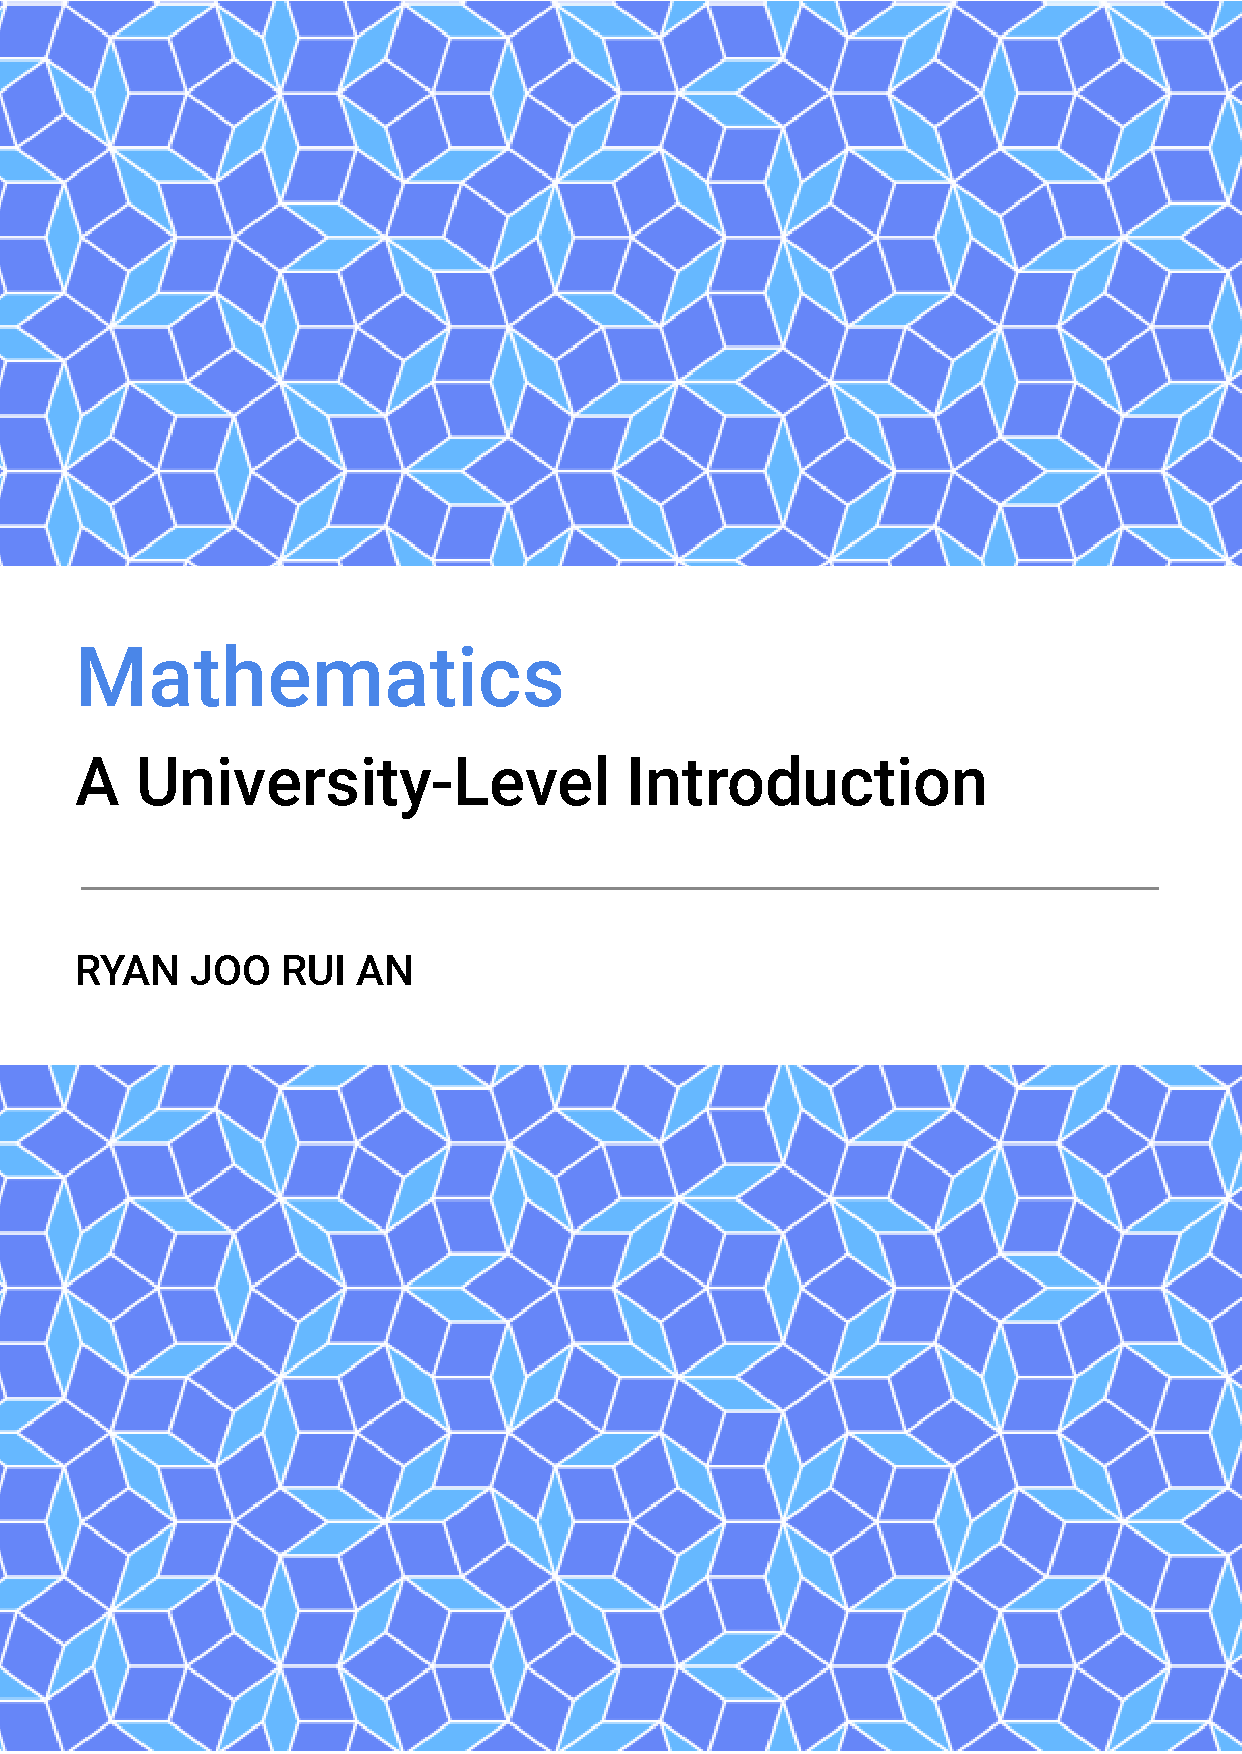
\includepdf{cover_page_uni}
% https://docs.google.com/document/d/1BnYV-5DkLfizphAaOHeH5S_hUeFZTAGS0Cg6YEeL7oA/edit?usp=sharing

\begin{titlepage}
\title{Mathematics:\\
A University-Level Introduction}
\author{Ryan Joo Rui An}
\date{Last updated: \today}
\end{titlepage}

\maketitle

\chapter*{Preface}
\begin{quote}
\textit{``The mathematician does not study mathematics because it is useful; he studies it because he delights in it and he delights in it because it is beautiful."}

\begin{flushright}--- Henri Poincar{\'e} (1854--1912)\\
French mathematician and theoretical physicist\end{flushright}
\end{quote}

\section*{About the author}
At this moment of writing, I am a high school student working on my A Level studies in Singapore. I have about 11 years of participating in Mathematics competitions, including three years of experience in mental arithmetic and the rest few years in Mathematics Olympiad.

\section*{About this book}
My initial purpose of writing this book was to summarise what I had learnt about university level Mathematics. The writing is intentionally kept simple, without large intimidating blocks of text, to ensure readability. 

\section*{Acknowledgements}
I am indebted to countless people for this work. Here is a partial (surely incomplete) list.
\begin{itemize}
\item Lecture notes by the University of Oxford, which can be found \href{https://courses.maths.ox.ac.uk/}{here}.
\item Lecture notes on MIT OpenCourseWare, which can be found \href{https://ocw.mit.edu/}{here}.
\item The authors of all the books I have referred to when writing this book.
\end{itemize}

\tableofcontents

% Materials to be cleared:
% https://www.seab.gov.sg/docs/default-source/national-examinations/syllabus/alevel/2022syllabus/9649_y22_sy.pdf
% https://www.cambridgeinternational.org/Images/597381-2023-2025-syllabus.pdf
\part{Introduction}
\chapter{Mathematical Reasoning and Logic}
% https://www.maths.ox.ac.uk/system/files/attachments/study_public_0.pdf

\section{Logical statements and notation}
Some terminology:
\begin{itemize}
\item \textbf{Definition}: a precise and unambiguous description of the meaning of a mathematical term. It characterizes the meaning of a word by giving all the properties and only those properties that must be true.

\item \textbf{Theorem}: a mathematical statement that is proved using rigorous mathematical reasoning. In a mathematical paper, the term theorem is often reserved for the most important results.

\item \textbf{Lemma}: a minor result whose sole purpose is to help in proving a theorem. It is a stepping stone on the path to proving a theorem. Very occasionally lemmas can take on a life of their own.

\item \textbf{Corollary}: a result in which the (usually short) proof relies heavily on a given theorem. We often say that ``this is a corollary of Theorem A".

\item \textbf{Proposition}: a proven and often interesting result, but generally less important than a theorem.

\item \textbf{Conjecture}: a statement that is unproved, but is believed to be true.

\item \textbf{Axiom/Postulate}: a statement that is assumed to be true without proof. These are the basic building blocks from which all theorems are proven.

\item \textbf{Identity}: a mathematical expression giving the equality of two (often variable) quantities.

\item \textbf{Paradox}: a statement that can be shown, using a given set of axioms and definitions, to be both true and false. Paradoxes are often used to show the inconsistencies in a flawed theory.
\end{itemize}

\subsection{Notation}
A proposition is a sentence which has exactly one truth value, i.e. it is either true or false, but not both and not neither. A proposition is denoted by uppercase letters such as $P$ and $Q$. If the proposition $P$ depends on a variable $x$, it is sometimes helpful to denote it by $P(x)$. 

\textbf{Equivalence:} $P \equiv Q$ means $P$ and $Q$ are logically equivalent statements.

\textbf{Conjunction:} $P \land Q$ means ``$P$ and $Q$".

\textbf{Disjunction:} $P \lor Q$ means ``$P$ or $Q$".

\textbf{Negation:} $\lnot P$ means ``not $P$".

\begin{itemize}
\item Double negation law:
\[ P \equiv \lnot(\lnot P) \]

\item Commutative property:
\[ P \land Q \equiv Q \land P \quad P \lor Q \equiv Q \lor P \]

\item Associative property for conjunction: 
\[ (P\land Q)\land R \equiv P\land (Q\land R) \]

\item Associative property for disjunction: 
\[ (P\lor Q)\lor R \equiv P\lor (Q\lor R) \]

\item Distributive property for conjunction across disjunction: 
\[ P\land(Q\lor R) \equiv (P\land Q)\lor(P\land Q) \]

\item Distributive property for disjunction across conjunction: 
\[ P\lor(Q\land R) \equiv (P\lor Q)\land(P\lor R) \]

\item \textbf{De Morgan's Laws}:
\[ \lnot(P \lor Q) \iff (\lnot P \land \lnot Q) \]
\[ \lnot (P\land Q) \iff (\lnot P\lor \lnot Q) \]
\end{itemize}

\begin{exmp}{}{}
Assume that $x$ is a fixed real number. What is the negation of the statement $1<x<2$?
\end{exmp}
\begin{solution}
The negation of $1<x<2$ is ``it is not the case that $1<x<2$”. This is not useful.

Note that $1<x<2$ means $1<x$ and $x<2$. Let $P:1<x$ and $Q:x<2$. Then the statement $1<x<2$ is $P \land Q$.

By De Morgan's Laws, we have $\lnot (P \land Q) \equiv \lnot P \lor \lnot Q$.

\textbf{Trichotomy Axiom of real numbers} states that given fixed real numbers $a$ and $b$, exactly one of the statements $a<b, a=b, b<a$ is true. Hence $\lnot P \equiv \lnot (1<x) \equiv (x \le 1)$ and $\lnot Q \equiv \lnot (x<2) \equiv (x \ge 2)$.

Thus
\[ \lnot (1<x<2) \equiv \lnot (P \land Q) \equiv \lnot P \lor \lnot Q \equiv (1 \ge x) \lor (x \ge 2). \]

Therefore the negation of $1<x<2$ is logically equivalent to the statement $x \le 1$ or $x \ge 2$.
\end{solution}

\begin{exmp}{}{}
Assume that $n$ is a fixed positive integer. Find a useful denial of the statement
\[ n = 2 \text{ or } n \text{ is odd.} \]
\end{exmp}
\begin{solution}
Using De Morgan's Laws,
\begin{align*}
\lnot [(n = 2) \lor (n \text{ is odd})] &\equiv \lnot(n = 2) \land \lnot(n \text{ is odd}) \\
&\equiv (n \neq 2) \land (n \text{ is even})
\end{align*}
where we are using the fact that every integer is either even or odd, but not both.

Thus a useful denial of the given statement is: $n$ is an even integer other than 2.
\end{solution}
\pagebreak

\textbf{Implication:} $P \implies Q$ means ``$P$ implies $Q$", i.e. if $P$ holds then $Q$ also holds. It is equivalent to saying ``If $P$ then $Q$". The only case when $P \implies Q$ is false is when the hypothesis $P$ is true and the conclusion $Q$ is false.

\begin{itemize}
\item $P \implies Q \equiv (\lnot P) \lor Q$.
\item $\lnot (P \implies Q) \equiv P \land (\lnot Q)$.
\end{itemize}

The \textbf{converse} of $P \implies Q$ is the statement $Q \implies P$.
\[ P \implies Q \not\equiv Q \implies P \]

The \textbf{contrapositive} of $P \implies Q$ is the statement $(\lnot Q) \implies (\lnot P)$.
\[ P \implies Q \equiv (\lnot Q) \implies (\lnot P) \]

\textbf{Bidirectional implication:} $P \iff Q$ means $P \implies Q$ and $Q \implies P$. We can read this as ``$P$ if and only if $Q$". The letters ``iff" are also commonly used to stand for ‘if and only if’.
\[ P \iff Q \equiv (P \implies Q) \land (Q \implies P) \]

\begin{itemize}
\item $P \iff Q$ is true exactly when $P$ and $Q$ have the same truth value.
\end{itemize}

\textbf{Quantifiers}: universal quantifier $\forall$ means ``for all" or ``for every", universal quantifier $\exists$ means ``there exists". For example, ``$\exists x \in S \suchthat P(x)$" can be read as ``there exists $x$ in $S$ such that $P(x)$ holds". A common variant is $\exists!$ which means ``there exists unique", implying that there is one, and only one, element with the given property.

These are versions of De Morgan's laws for quantifiers:
\[ \lnot \forall x\,P(x) \iff \exists x\,\lnot P(x) \]
\[ \lnot \exists x\,P(x) \iff \forall x\,\lnot P(x) \]

\begin{exmp}{}{}
Find a useful denial of the statement
\[ \text{for all real numbers } x, \text{ if } x>2, \text{ then } x^2>4 \]
\end{exmp}
\begin{solution}
In logical notation, this statement is $(\forall x \in \RR)[x>2 \implies x^2>4]$.
\begin{align*}
\lnot\{(\forall x \in \RR)[x>2 \implies x^2>4]\} 
&\equiv (\exists x \in \RR) \lnot[x>2 \implies x^2>4] \\
&\equiv (\exists x \in \RR) \lnot [(x\le2) \lor (x^2>4)] \\
&\equiv (\exists x \in \RR) [(x>2) \land (x^2\le4)]
\end{align*}
Therefore a useful denial of the statement is:
\[ \text{there exists a real number } x \text{ such that } x>2 \text{ and } x^2\le4. \] 
\end{solution}

\begin{remark}
Regardless of how much you use these symbols in your own writing, it is important to understand and be fluent in interpreting these symbols in other people's writing.
\end{remark}
\pagebreak

\subsection{Handling logical statements}
\subsubsection{If, only if, $\implies$}
Statements of this form are probably the most common, although they may sometimes appear quite differently. The following all mean the same thing:
\begin{enumerate}[label=(\roman*)]
\item if $P$ then $Q$;
\item $P$ implies $Q$;
\item $P \implies Q$;
\item $P$ only if $Q$;
\item $P$ is a sufficient condition for $Q$;
\item $Q$ is a necessary condition for $P$;
\item whenever $P$ holds, $Q$ also holds;
\item if $Q$ does not hold then $P$ does not hold;
\item not $Q$ implies not $P$;
\item $\lnot Q \implies \lnot P$.
\end{enumerate}

The last three of these are known as the \textbf{contrapositive}.

\textbf{How to prove:} To prove $P \implies Q$, start by assuming that $P$ holds and try to deduce through some logical steps that $Q$ holds too. Alternatively, start by assuming that $Q$ does not hold and show that $P$ does not hold (that is, we prove the contrapositive).

\begin{remark}
Note that the contrapositive is not the same as the converse. The contrapositive of $P \implies Q$ is $\lnot Q \implies \lnot P$; it is simply a different way of stating exactly the same thing. But the converse of $P \implies Q$ is $Q \implies P$, which means something completely different.
\end{remark}

\subsubsection{If and only if, iff, $\iff$}
These statements are usually best thought of separately as ‘if’ and ‘only if’ statements.

\textbf{How to prove:} To prove $P \iff Q$, prove the statement in both directions, i.e. prove both $P \implies Q$ and $Q \implies P$. Remember to make very clear, both to yourself and in your written proof, which direction you are doing.

\subsubsection{Quantifiers}
The quantifiers $\forall$ and $\exists$ are probably the most challenging of the notation. Do practice reading statements that include these symbols and checking that you understand their meaning.

\textbf{How to prove:} To prove a statement of the form $\forall x \in X \suchthat P(x)$’, start the proof with ‘Let $x \in X$.’ or ‘Suppose $x \in X$ is given.’ to address the quantifier with an arbitrary $x$; provided no other assumptions about $x$ are made during the course of proving $P(x)$, this will prove the statement for all $x \in X$. 

To prove a statement of the form $\exists x \in X \suchthat P(x)$, there is not such a clear steer about how to continue: you may need to show the existence of an $x$ with the right properties; you may need to demonstrate logically that such an $x$ must exist because of some earlier assumption, or it may be that you can show constructively how to find one; or you may be able to prove by contradiction, supposing that there is no such $x$ and consequently arriving at some inconsistency.

\begin{remark}
Read from left to right, and as new elements or statements are introduced they are allowed to depend on previously introduced elements but cannot depend on things that are yet to be mentioned.
\end{remark}

\begin{remark}
To avoid confusion, it is a good idea to keep to the convention that the quantifiers come first, before any statement to which they relate.
\end{remark}

\subsubsection{Negation}
For a statement $P$, the negated statement $\lnot P$ is the statement that is false when $P$ is true, and true when $P$ is false. It is important to be adept at negating statements (in order to seek contradictions, for example). For a simple statement such as $x \in S$, the negation is simply $x \notin S$. For more involved statements, it can be more confusing.

For statements in the form of $P \implies Q$, the negated statement is $P \not\implies Q$. Since $P \implies Q$ means that $Q$ is true whenever $P$ is true, $P \not\implies Q$ means that (at least in some circumstance) $P$ is true and $Q$ is not true. Proving $P \not\implies Q$ would typically involve demonstrating such a circumstance.

For statements involving quantifiers, the negation of $\forall x \in X, P(x)$ is $\exists x \in X, \lnot P(x)$ (since, if it is not true that $P(x)$ holds for every $x$, then it must be the case that there is some $x$ for which $P(x)$ does not hold). Similarly, the negation of $\exists x \in X, P(x)$ is $\forall x \in X, \lnot P(x)$ (since, if it is not true that there is an $x$ for which $P(x)$ holds, then it means that $P(x)$ does not hold for any $x$).\footnote{This is essentially an instance of De Morgan's laws.}
\pagebreak

\section{Proofs}
\subsection{Direct proof}
To prove $P \implies Q$ directly, we make use of $P$ to arrive at $Q$ through a sequence of logical reasoning. It may be that we can start from $P$ and work directly to $Q$, or it may be that we make use of $P$ along the way.

\subsection{Proof by contradiction}
To prove $P \implies Q$ by contradiction, we suppose that $Q$ is not true and show through some logical reasoning (making use of the hypotheses $P$) that this leads to a contradiction or inconsistency. We may arrive at something that contradicts the hypotheses $P$, or something that contradicts the initial supposition that $Q$ is not true, or we may arrive at something that we know to be universally false.

\begin{exmp}{Irrationality of $\sqrt{2}$}{}
Prove that $\sqrt{2}$ is irrational.
\end{exmp}
\begin{proof}
We prove by contradiction. Suppose otherwise, that $\sqrt{2}$ is rational. Using the definition of rational numbers, we can write it as $\sqrt{2} = \dfrac{a}{b}$ for some $a,b\in\ZZ,b\neq 0$. 

We also assume that $\dfrac{a}{b}$ is simplified to lowest terms, since that can obviously be done with any fraction. Notice that in order for $\dfrac{a}{b}$ to be in simplest terms, both $a$ and $b$ cannot be even; one or both must be odd, otherwise we could simplify the fraction further.

Squaring both sides gives us
\[ a^2 = 2b^2. \]
Since RHS is even, LHS must also be even. Hence it follows that $a$ is even. Let $a=2k$ where $k\in\ZZ$. Substituting $a = 2k$ into the above equation and simplifying it gives us
\[ b^2=2k^2. \]
This means that $b^2$ is even, from which follows again that $b$ is even. 

This is a contradiction, as we started out assuming that $\dfrac{a}{b}$ was simplified to lowest terms, and now it turns out that $a$ and $b$ both would be even. Hence proven.
\end{proof}

\subsection{Proof by induction}
The following principle is sometimes quoted as a theorem, although it follows directly from our definition of the natural numbers.
\begin{thrm}{Principle of Induction}{}
Let $P(n)$ be a family of statements indexed by the natural numbers. Suppose that 
\begin{enumerate}[label=(\roman*)]
\item $P(1)$ is true and
\item for all $m \in \NN$, if $P(m)$ is true then $P(m+1)$ is also true.
\end{enumerate}
 Then $P(n)$ is true for all $n \in \NN$.
\end{thrm}

Using logic notation, this is written as
\[ \{P(1) \land (\forall n \in \ZZ^+) [P(m) \implies P(m+1)]\} \implies (\forall n \in \ZZ^+)P(n) \] 

Induction is often visualised like toppling dominoes. The \textbf{inductive step} (ii) corresponds to placing each domino sufficiently close that it will be hit when the previous one falls over, and the initial step, (i) -- known as the \textbf{base case} -- corresponds to knocking over the first one.

\begin{exmp}{}{}
Prove that for any $n \in \NN$,
\[ \sum_{k=1}^n k = \frac{n(n+1)}{2} \]
\end{exmp}

\begin{proof}
Clearly $P(1)$ holds because for $n=1$, the sum on the LHS is 1 and the expression on the RHS is also 1.

Now suppose $P(n)$ holds. Then
\begin{align*}
\sum_{k=1}^{n+1} k &= \sum_{k=1}^n k + (n+1) \\
&= \frac{n(n+1)}{2} + (n+1) \\
&= \frac{(n+1)(n+2)}{2}
\end{align*}
which is exactly the statement $P(n+1)$. So by induction, $P(n)$ is true for all $n \in \NN$.
\end{proof}

A corollary\footnote{an extension of, or a consequence of, a theorem or proposition; a corollary is generally not such a major result as the theorem or proposition itself.} of induction is if the family of statements holds for $n \ge N$, rather than necessarily $n \ge 0$:

\begin{corollary}
Let $N$ be an integer and let $P(n)$ be a family of statements indexed by integers $n \ge N$. Suppose that 
\begin{enumerate}[label=(\roman*)]
\item $P(N)$ is true and
\item for any $n \ge N$, if $P(n)$ is true then $P(n+1)$ is also true. 
\end{enumerate}
Then $P(n)$ is true for all $n \ge N$.
\end{corollary}

\begin{proof}
This follows directly by applying the above theorem to the statement $Q(n) = P(n+N)$ for $n \in N$.
\end{proof}

Another variant on induction is when the inductive step relies on some earlier case(s) but not necessarily the immediately previous case. This is sometimes \textbf{strong induction}:

\begin{thrm}{Strong Form of Induction}{}
Let $P(n)$ be a family of statements indexed by the natural numbers. Suppose that
\begin{enumerate}[label=(\roman*)]
\item $P(1)$ is true and
\item for all $m \in \NN$, if for integers $k$ with $1 \le k \le m$, $P(k)$ is true then $P(m+1)$ is true.
\end{enumerate}
Then $P(n)$ is true for all $n \in \NN$.
\end{thrm}

Using logic notation, this is written as
\[ \{P(1) \land (\forall m \in \ZZ^+) [P(1) \land P(2) \land \cdots \land P(m) \implies P(m+1)]\} \implies (\forall n \in \ZZ^+)P(n) \]

\begin{proof}
We can this it to an instance of ``normal" induction by defining a related family of statements $Q(n)$. 

Let $Q(n)$ be the statement ``$P(k)$ holds for $k=0,1,\dots,n$". Then the conditions for the strong form are equivalent to 
\begin{enumerate}[label=(\roman*)]
\item $Q(0)$ holds and 
\item for any $n$, if $Q(n)$ is true then $Q(n+1)$ is also true.
\end{enumerate}
It follows by induction that $Q(n)$ holds for all $n$, and hence $P(n)$ holds for all $n$.
\end{proof}

The following example illustrates how the strong form of induction can be useful:

\begin{exmp}{Fundamental Theorem of Arithmetic}{}
Every natural number greater than 1 may be expressed as a product of one or more prime numbers.
\end{exmp}

\begin{proof}
Let $P(n)$ be the statement that $n$ may be expressed as a product of prime numbers. 

Clearly $P(2)$ holds, since $2$ is itself prime. 

Let $n \ge 2$ be a natural number and suppose that $P(m)$ holds for all $m<n$.

\begin{itemize}
\item If $n$ is prime then it is trivially the product of the single prime number $n$. 

\item If $n$ is not prime, then there must exist some $r, s > 1$ such that $n = rs$. By the inductive hypothesis, each of $r$ and $s$ can be written as a product of primes, and therefore $n = rs$ is also a product of primes.
\end{itemize}

Thus, whether $n$ is prime or not, we have have that $P(n)$ holds. By strong induction, $P(n)$ is true for all natural numbers. That is, every natural number greater than 1 may be expressed as a product of one or more primes.
\end{proof}

Cauchy induction
\pagebreak

\begin{prbm}[FM/TJC/2023]
Prove by mathematical induction, for $n \ge 2$,
\[ \sqrt[n]{n}<2 - \frac{1}{n}. \]
\end{prbm}

\begin{proof}
Let $P(n)$ be the proposition that $\sqrt[n]{n}<2 - \dfrac{1}{n}$ for $n \ge 2$.

When $n=2$, $\sqrt{2} <2-\dfrac{1}{2}=1.5$ which is true. Hence $P(2)$ is true.

Assume $P(k)$ is true for $k \ge 2, k \in \ZZ^+$, i.e.
\[ \sqrt[k]{k}<2 - \dfrac{1}{k} \implies k<\brac{2-\frac{1}{k}}^k \]

We want to prove that $P(k+1)$ is true, i.e.
\[ k+1<\brac{2-\frac{1}{k+1}}^{k+1} \]

Since $k>2$, we have 
\begin{align*}
\brac{2-\frac{1}{k+1}}^{k+1}
&> \brac{2-\frac{1}{k}}^{k+1} \quad \because k>2 \\
&= \brac{2-\frac{1}{k}}^k\brac{2-\frac{1}{k}} \\
&> k\brac{2-\frac{1}{k}} \quad \text{by inductive hypothesis} \\
&= 2k-1 = k+k-1 > k-1 \because k>2
\end{align*}
Hence $P(k+1)$ is true.

Since $P(2)$ is true and $P(k)\implies P(k+1)$, by mathematical induction $P(n)$ is true.
\end{proof}
\pagebreak

\begin{prbm}
Prove that for all integers $n \ge 3$, 
\[ \brac{1+\frac{1}{n}}^n<n \]
\end{prbm}

\begin{proof}
Suppose for an integer $k$, we have 
\[ \brac{1+\frac{1}{k}}^k<k \]
Then
\[ \brac{1+\frac{1}{k}}^k\brac{1+\frac{1}{k}} = \brac{1+\frac{1}{k}}^{k+1}<k\brac{1+\frac{1}{k}} = k+1  \]
Note 
\[ \brac{1+\frac{1}{k}}^{k+1} > \brac{1+\frac{1}{k+1}}^{k+1} \quad \text{since } k<k+1 \iff \frac{1}{k}>\frac{1}{k+1} \]
The rest of the proof follows easily.
\end{proof}
\pagebreak

\subsection{Counterexamples}
Providing a counterexample is the best method for refuting, or dispoving, a conjecture. 

In seeking counterexamples, it is a good idea to keep the cases you consider simple, rather than searching randomly. It is often helpful to consider ``extreme" cases; for example, something is zero, a set is empty, or a function is constant.

\chapter{Set Theory}
\section{Basics}
\subsection{Notation}
You should, by now, be familiar with the following definitions and notation:
\begin{itemize}
\item A \vocab{set} $S$ can be loosely defined as a collection of objects.

\item For a set $S$, we write $x \in S$ to mean that $x$ is an \vocab{element} of $S$, and $x \notin S$ if otherwise.

\item A set can be defined in terms of some property $P(x)$ that the elements $x \in S$ satisfy, denoted by 
\[ \{x \in S \mid P(x)\} \]

\item Some basic sets (of numbers) you should be familiar with:
\begin{itemize}
\item $\NN=\{0,1,2,3,\dots\}$ denotes the natural numbers (non-negative integers).
\item $\ZZ=\{\dots,-2,-1,0,1,2,\dots\}$ denotes the integers.
\item $\QQ=\{\frac{p}{q} \mid p,q\in\ZZ, q\neq0\}$ denotes the rational numbers.
\item $\RR$ denotes the real numbers, which can be expressed in terms of decimal expansion.
\item $\CC=\{x+yi \mid x,y\in\RR\}$ denotes the of complex numbers.
\end{itemize}

\item The \vocab{empty set} is the set with no elements, denoted by $\emptyset$.

\item $A$ is a \vocab{subset} of $B$ if every element of $A$ is in $B$, denoted by $A \subseteq B$.
\[ A \subseteq B \iff \forall x, x\in A \implies x\in B \]

$\subseteq$ is transitive, i.e. if $A \subseteq B$ and $B \subseteq C$, then $A \subseteq C$.
\begin{proof}
Let $x\in A$. 
Since $A \subseteq B$ and $x\in A$, $x\in B$. 
Since $B \subseteq C$ and $x\in B$, $x\in C$. 
Hence $A \subseteq C$.
\end{proof}

$A$ is a \vocab{proper subset} of $B$ if $A \subseteq B$ and $A \neq B$, denoted by $A \subset B$.

Using this definition, we have the relationship 
\[ \NN \subset \ZZ \subset \QQ \subset \RR \]

\item $A$ and $B$ are \vocab{equal} if and only if they contain the same elements, denoted by $A=B$.

To prove that $A$ and $B$ are equal, we simply need to prove that $A \subseteq B$ and $A \subseteq B$.

\begin{proof}
We have 
\begin{align*}
A = B &\iff (\forall x)[x \in A \iff x \in B] \\
&\iff (\forall x)[(x \in A \implies x \in B) \land (x \in B \implies x \in A)] \\
&\iff \{(\forall x)[x \in A \implies x \in B]\} \land {(\forall x)[x \in B \implies x \in A)]} \\
&\iff (A \subseteq B) \land (B \subseteq A)
\end{align*}
\end{proof}

\item Some frequently occurring subsets of the real numbers are known as \vocab{intervals}, which can be visualised as sections of the real line:
\begin{itemize}
\item Open interval
\[ (a,b) = \{x\in\RR \mid a<x<b\} \]
\item Closed interval
\[ [a,b] = \{x\in\RR \mid a\le x<b\} \]
\item Half open interval
\[ (a,b] = \{x\in\RR \mid a<x\le b\} \]
\end{itemize}

\item The \vocab{power set} $\mathcal{P}(A)$ of $A$ is the set of all subsets of $A$ (including the set itself and the empty set).

\item An \vocab{ordered pair} is denoted by $(a,b)$, where the order of the elements matters. Two pairs $(a_1,b_1)$ and $(a_2,b_2)$ are equal if and only if $a_1=a_2$ and $b_1=b_2$. 

Similarly, we have ordered triples $(a,b,c)$, quadruples $(a,b,c,d)$ and so on. If there are $n$ elements it is called an $n$-tuple.

\item The \vocab{Cartesian product} of sets $A$ and $B$, denoted by $A \times B$, is the set of all ordered pairs with the first element of the pair coming from $A$ and the
second from $B$:
\begin{equation}
A \times B = \{(a,b) \mid a \in A, b \in B\}
\end{equation}
If $A = B$, we write $A \times A$ as $A^2$. Note that the case where $A = B = \RR$ is a particularly important one as $\RR^2$ represents the two-dimensional real plane.

More generally, we define $A_1 \times A_2 \times \cdots \times A_n$ to be the set of all ordered $n$-tuples $(a_1, a_2, \dots, a_n)$, where $a_i \in A_i$ for $1 \le i \le n$. If all the A$_i$ are the same, we write the product as $A^n$.

\begin{exmp}{}{}
$\RR^2$ is the Euclidean plane, $\RR^3$ is the Euclidean space, and $\RR^n$ is the $n$-dimensional Euclidean space.
\begin{align*}
\RR \times \RR = \RR^2 &= \{(x,y) \mid x,y \in \RR\} \\
\RR \times \RR \times \RR = \RR^3 &= \{(x,y,z) \mid x,y,z \in \RR\} \\
\RR^n &= \{(x_1,x_2,\dots,x_n) \mid x_1,x_2,\dots,x_n \in \RR\}
\end{align*}
\end{exmp}
\end{itemize}

\subsection{Algebra of Sets}
Given $A \subset S$ and $B \subset S$.
\begin{itemize}
\item The \vocab{union} $A \cup B$ is the set consisting of elements that are in $A$ or $B$ (or both):
\[ A\cup B=\{x \in S \mid x\in A \lor x\in B\} \]

\item The \vocab{intersection} $A \cap B$ is the set consisting of elements that are in both $A$ and $B$:
\[ A\cap B=\{x \in S \mid x\in A \land x\in B\} \]

$A$ and $B$ are \vocab{disjoint} if both sets have no element in common:
\[ A\cap B = \emptyset \]

More generally, we can take unions and intersections of arbitrary numbers of sets, even infinitely many. If we have a family of subsets $\{A_i \mid i \in I\}$, where $I$ is an \textbf{indexing set}, we write
\[ \bigcup_{i\in I} A_i = \{x \mid \exists i\in I\,(x\in A_i)\} \]
and
\[ \bigcap_{i\in I} A_i = \{x \mid \forall i\in I\,(x\in A_i)\} \] 

\item The \vocab{complement} of $A$, denoted by $A^c$ or $A^\prime$, is the set containing elements that are not in A:
\[ A^c = \{x \in S \mid x \notin A\} \]

\item The \vocab{set difference}, or complement of $B$ in $A$, written $A\setminus B$, is the subset consisting of those elements that are in $A$ and not in $B$:
\[ A\setminus B = \{x \in A \mid x \notin B\} \]
Note that $A\setminus B = A \cap B^c$.
\end{itemize}

\begin{proposition}[Double Inclusion]
Let $A\subset S$ and $B\subset S$. Then 
\begin{equation}
A = B \iff A \subseteq B \text{ and } B \subseteq A
\end{equation}
\end{proposition}
\begin{proof} We prove both directions.

\textbf{Forward direction:}

If $A = B$, then every element in $A$ is an element in $B$, so certainly $A \subseteq B$, and
similarly $B \subseteq A$. 

\textbf{Backward direction:}

Suppose $A \subseteq B$, and $B \subseteq A$. Then for every element $x \in S$, if $x \in A$ then $A \subseteq B$ implies that $x \in B$, and if $x \notin A$ then $B \subseteq A$ means $x \notin B$. So $x \in A$ if and only if $x \in B$, and therefore $A = B$.
\end{proof}

\begin{proposition}[Distributive Laws]
Let $A\subset S$, $B\subset S$ and $C\subset S$. Then
\begin{equation}
(A\cup B)\cap C = (A\cap C)\cup(B\cap C)
\end{equation}
\begin{equation}
(A\cap B)\cap C = (A\cup C)\cap(B\cup C)
\end{equation}
\end{proposition}
\begin{proof}
For the first one, suppose $x$ is in the LHS, that is $x \in A\cup(B \cap C)$. This means that $x \in A$ or $x \in B \cap C$ (or both). Thus either $x \in A$ or $x$ is in both $B$ and $C$ (or $x$ is in all three sets). If $x \in A$ then $x \in A\cup B$ and $x \in A\cup C$, and therefore $x$ is in the RHS. If $x$ is in both $B$ and $C$ then similarly $x$ is in both $A\cup B$ and $A\cup C$. Thus every element of the LHS is in the RHS, which means we have shown $A \cup (B \cap C) \subseteq (A \cup B) \cap (A \cup C)$.

Conversely suppose that $x \in (A \cup B) \cap (A \cup C)$. Then $x$ is in both $A \cup B$ and $A\cup C$. Thus either $x \in A$ or, if $x \notin A$, then $x \in B$ and $x \in C$. Thus $x \in A\cup(B \cap C)$. Hence $(A \cup B) \cap (A \cup C) \subseteq A \cup (B \cap C)$.

By double inclusion, $(A \cup B) \cap (A \cup C) = A \cup (B \cap C)$.

The proof of the second one follows similarly and is left as an exercise.
\end{proof}

\begin{proposition}[De Morgan's Laws]
Let $A \subset S$ and $B \subset S$. Then
\begin{equation}
(A \cup B)^c = A^c \cap B^c
\end{equation}
\begin{equation}
(A \cap B)^c = A^c \cup B^c
\end{equation}
\end{proposition}
\begin{proof}
For the first one, suppose $x \in (A \cup B)^c$. Then $x$ is not in either $A$ or $B$. Thus $x \in A^c$ and $x \in B^c$, and therefore $x \in A^c \cap B^c$. 

Conversely, suppose $x \in A^c \cap B^c$. Then $x \notin A$ and $x \notin B$, so $x$ is in neither $A$ nor $B$, and therefore $x \in (A \cup B)^c$.

By double inclusion, the first result holds. The second result follows similarly and is left as an exercise.
\end{proof}

De Morgan’s laws extend naturally to any number of sets, so if $\{A_i \mid i \in I\}$ is a family of subsets of $S$, then
\[ \brac{\bigcap_{i\in I}A_i}^c = \bigcup_{i\in I}A_i^c \quad \text{and} \quad \brac{\bigcup_{i\in I}A_i}^c = \bigcap_{i\in I}A_i^c \]

\begin{prbm}
Let $A$ be the set of all complex polynomials in $n$ variables. Given a subset $T \subset A$, define the \textit{zeros} of $T$ as the set
\[ Z(T) = \{P=(a_1,\dots,a_n) \mid f(P)=0 \text{ for all } f \in T\} \]
A subset $Y \in \CC^n$ is called an algebraic set if there exists a subset $T \subset A$ such that $Y=Z(T)$.

Prove that the union of two algebraic sets is an algebraic set.
\end{prbm}
\begin{proof}
We would like to consider $T=\{f_1, f_2, \dots\}$ expressed as indexed sets $T=\{f_i\}$. Then $Z(T)$ can also be expressed as $\{P \mid \forall i, f_i(P)=0\}$.

Suppose that we have two algebraic sets $X$ and $Y$. Let $X=Z(S)$, $Y=Z(T)$ where $S,T$ are subsets of $A$ (basically, they are certain sets of polynomials). Then
\[ X=\{P \mid \forall f \in S, f(P)=0\} \]
\[ Y=\{P \mid \forall g \in T, g(P)=0\} \]

We imagine that for $P\in X\cap Y$, we have $f(P)=0$ or $g(P)=0$. Hence we consider the set of polynomials
\[ U=\{f\cdot g \mid f\in S, g\in T\} \]

For any $P\in X\cup Y$ and for any $fg\in U$ where $f\in S$ and $f\in g$, either $f(P)=0$ or $g(P)=0$, hence $fg(P)=0$ and thus $P\in Z(U)$.

On the other hand if $P\in Z(U)$, suppose otherwise that $P$ is not in $X\cup Y$, then $P$ is neither in $X$ nor in $Y$. This means that there exists $f\in S,g\in T$ such that $f(P)\neq0$ and $g(P)\neq0$, hence $fg(P)\neq0$. This is a contradiction as $P\in Z(U)$ implies $fg(P)=0$. Hence we have $X\cup Y=Z(U)$ and thus $X\cup Y$ is an algebraic set.

Now the other direction is simpler and can actually be generalised: The intersection of arbitrarily many algebraic sets is algebraic. 

The basic result is that if $X=Z(S)$ and $Y=Z(T)$ then $X\cap Y=Z(S\cup T)$. 

This is the beginning of a subject called algebraic geometry, which discusses about the geometry of algebraic surfaces, namely those kinds of surfaces defined by zeroes of polynomials (conic sections for example).
\end{proof}

\subsection{Cardinality}
Informally, the \vocab{cardinality} of $S$, denoted $|S|$, is a measure of its ``size".

We will be able to give a nicer definition of cardinality later, once we have discussed bijections, but the following provides a recursive definition of the cardinality for a finite set:

\begin{defn}{Finiteness and the cardinality of a finite set}{}
The empty set $\emptyset$ is
finite with $|\emptyset|=0$. $S$ is finite with $|S|= n+1$, if there exists $s \in S$ such that $|S\setminus \{s\}| = n$ for some $n \in \NN$. We call $|S|$ the \vocab{cardinality} of $S$. Any set that is not finite is said to be infinite.
\end{defn}

It is not hard to see that this means that if $S = \{x_1,x_2,\dots,x_n\}$, and $x_i \neq x_j$ whenever $i \neq j$, then $|S| = n$. Conversely, if $|S| = n$ then $S$ is a set with $n$ elements.

\begin{proposition}
Let $A$ and $B$ be finite sets. Then $|A \cup B| = |A| + |B| - |A \cap B|$.
\end{proposition}

\begin{proof}
The proof is left as an exercise.
\end{proof}

\begin{proposition}[Subsets of a finite set]
If a set $A$ is finite with $|A| = n$, then its power set has $|\mathcal{P}(A)| = 2^n$.
\end{proposition}

\begin{proof}
We use induction. For the initial step, note that if $|A| = 0$ then $A = \emptyset$ has no elements, so there is a single subset $\emptyset$, and therefore $|\mathcal{P}(A)| = 1 = 2^0$.

Now suppose that $n \ge 0$ and that $|P(S)| = 2^n$ for any set S with $|S| = n$. Let $A$ be any set with $|A| = n+1$. By definition, this means that there is an element $a$ and a set $A_0 = A\setminus\{a\}$ with $|A_0| = n$. Any subset of A must either contain the element a or not, so we can partition $\mathcal{P}(A) = P(A_0) \cup \{S \cup \{a\} \mid S \in P(A_0)\}$. These two sets are disjoint, and each of them has cardinality $|P(A_0)| = 2^n$ by the inductive hypothesis. Hence $|\mathcal{P}(A)| = 2^n + 2^n = 2^{n+1}$.

Thus, by induction, the result holds for all $n$.
\end{proof}

Another way to see this is through combinatorics: Consider the process of creating a subset. We can do this systematically by going through each of the $|A|$ elements in $A$ and making the yes/no decision whether to put it in the subset. Since there are $|A|$ such choices, that yields $2^{|A|}$ different combinations of elements and therefore $2^{|A|}$ different subsets.

\pagebreak

\section{Relations}
\subsection{Definition}
A relation is a set of ordered pairs.

\begin{defn}{Relation}{}
$R$ is a \vocab{relation} between $A$ and $B$ if and only if $R$ is a subset of the Cartesian product $A \times B$, i.e. $R \subseteq A \times B$.

$a \in A$ and $b \in B$ are \textbf{related} if $(a,b) \in R$, denoted by $a R b$.
\end{defn}

Visually speaking, a relation is uniquely determined by a simple bipartite graph over $A$ and $B$. On the bipartite graph, this is usually represented by an edge between $a$ and $b$.

\begin{defn}{Binary relation}{}
A \vocab{binary relation} in $A$ is a relation between $A$ and itself, i.e. $R \subseteq A \times A$.
\end{defn}

$A$ and $B$ are the \vocab{domain} and \vocab{range} of $R$ respectively, denoted by $\dom R$ and $\ran R$ respectively, if and only if $A \times B$ is the smallest Cartesian product of which $R$ is a subset.

\begin{exmp}{}{}
$R = \{(1,a), (1,b), (2,b), (3,b)\}$, then 
\begin{itemize}
\item $\dom R = \{1,2,3\}$
\item $\ran R = \{a,b\}$
\end{itemize}
\end{exmp}

In many cases we do not actually use $R$ to write the relation because there is some other conventional notation:

\begin{exmp}{}{}
\begin{itemize}
\item The ``less than or equal to" relation $\le$ on the set of real numbers is $\{(x,y) \in \RR^2 \mid x \le y\}$. We write $x \le y$ if $(x,y)$ is in this set.
\item The ``divides" relation $\mid$ on $\NN$ is $\{(m,n) \in \NN^2: m \text{ divides } n\}$. We write $m \mid n$ if $(m,n)$ is in this set.
\item For a set S, the ``subset" relation $\subseteq$ on $\mathcal{P}(S)$ is $\{(A,B) \in \mathcal{P}(S)^2 \mid A \subseteq B\}$. We write $A \subseteq B$ if $(A,B)$ is in this set.
\end{itemize}
\end{exmp}
\pagebreak

\subsection{Properties of relations}
Let $A$ be a set, $R$ a relation on $A$, and $x,y,z \in A$. We say that
\begin{itemize}
\item $R$ is \textbf{reflexive} if $xRx$ for all $x$ in $A$.
\item $R$ is \textbf{symmetric} if whenever $xRy$ then $yRx$.
\item $R$ is \textbf{anti-symmetric} if whenever $xRy$ and $yRx$ then $x = y$.
\item $R$ is \textbf{transitive} if whenever $xRy$ and $yRz$ then $xRz$.
\end{itemize}

\begin{exmp}{Less than or equal to}{}
The relation $\le$ on $R$ is reflexive, anti-symmetric, and transitive, but not symmetric. 
\end{exmp}

More generally, any relation on $A$ that is reflexive, anti-symmetric, and transitive is called a \textbf{partial order}, denoted by $\le$. It is called a \textbf{total order} if for every $x, y \in A$, either $xRy$ or $yRx$ (or both).

\begin{exmp}{Less than}{}
The relation $<$ on $R$ is not reflexive, symmetric, or anti-symmetric, but it is transitive.
\end{exmp}

\begin{exmp}{Not equal to}{}
The relation $\neq$ on $R$ is not reflexive, anti-symmetric or transitive, but it is symmetric.
\end{exmp}

\begin{exmp}{Congruence modulo $n$}{}
Let $n \ge 2$ be an integer, and define $R$ on $\ZZ$ by saying $aRb$ if and only if $a-b$ is a multiple of $n$. Then $R$ is reflexive, symmetric and transitive.
\end{exmp}
\begin{proof} \
\begin{itemize}
\item Reflexivity: For any $a \in \ZZ$ we have $aRa$ as 0 is a multiple of $n$.
\item Symmetry: If $aRb$ then $a-b=kn$ for some integer $k$. So $b-a=-kn$, and hence $bRa$.
\item Transitivity: If $aRb$ and $bRc$ then $a-b=kn$ and $b-c=ln$ for integers $k,l$. So then $a-c=(a-b)+(b-c)=(k+l)n$, and hence $aRc$.
\end{itemize}
\end{proof}
\pagebreak

\subsection{Equivalence relations, equivalence classes, and partitions}
One important type of relation is an equivalence relation. An equivalence relation is a way of saying two objects are, in some particular sense, ``the same".

\begin{defn}{Equivalence relation}{}
A binary relation $R$ on $A$ is an \vocab{equivalence relation} if it is reflexive, symmetric and transitive. If $R$ is an equivalence relation, we denote it by $\sim$.
\end{defn}

\begin{remark}
We use the symbol $\sim$ to denote the equivalence relation $R$ in $A \times A$, and whenever $(a,b)\in R$ we denote $a \sim b$.
\end{remark}

An equivalence relation provides a way of grouping together elements that can be viewed as being the same:

\begin{defn}{Equivalence class}{}
Given an equivalence relation $\sim$ on a set $A$, and given $x \in A$, the \vocab{equivalence class} of $x$, denoted $[x]$, is the subset
\[ [x] = \{y \in A \mid y \sim x\} \]
\end{defn}

\begin{exmp}{Congruence modulo $n$}{}
For the equivalence relation of congruence modulo $n$, the equivalence class of 1 is the set $1 = \{\dots, -n+1, 1, n+1, 2n+1, \dots\}$; that is, all the integers that are congruent to 1 modulo $n$.
\end{exmp}

Properties of equivalence classes:
\begin{itemize}
\item Every two equivalence classes are disjoint
\item The union of equivalence classes form the entire set
\end{itemize}

You can translate these properties into the point of view from the elements: Every element belongs to one and only one equivalence class.
\begin{itemize}
\item No element belongs to two distinct classes
\item All elements belong to an equivalence class
\end{itemize}

\begin{defn}{Set of equivalence classes}{}
The \vocab{set of equivalence classes} (quotient sets) are the set of all equivalence classes, denoted by $A/\sim$.
\end{defn}

Grouping the elements of a set into equivalence classes provides a partition of the set, which we define as follows:

\begin{defn}{Partition}{}
A \vocab{partition} of a set $A$ is a collection of subsets $\{A_i \subseteq A \mid i \in I\}$, where $I$ is an indexing set, with the property that
\begin{enumerate}[label=(\roman*)]
\item $A_i \neq \emptyset$ for all $i \in I$ (that is, all the subsets are non-empty),
\item $\bigcup_{i\in I} Ai = A$ (that is, every member of $A$ lies in one of the subsets),
\item $A_i \cap A_j = \emptyset$ for every $i \neq j$ (that is, the subsets are disjoint).
\end{enumerate}
The subsets are called the parts of the partition.
\end{defn}

\begin{exmp}{Odd and even natural numbers}{}
$\{\{n \in \NN \mid n \text{ is divisible by } 2\}, \{n \in \NN \mid n+1 \text{ is divisible by } 2\}\}$ forms a partition of the natural numbers, into evens and odds.
\end{exmp}
\pagebreak

\begin{prbm}[Modular Arithmetic]
Define the ring of integers modulo $n$:
\[ \ZZ/n\ZZ = \ZZ/\sim \text{ where } x \sim y \iff x-y \in n\ZZ. \]
The equivalence classes are called congruence classes modulo $n$.
\begin{enumerate}[label=(\alph*)]
\item Define the sum of two congruence classes modulo $n$, $[x], [y] \in \ZZ/n\ZZ$, by
\[ [x] + [y] = [x + y] \]
Show that the above definition is well-defined.
\item Define the product of two congruence classes modulo $n$ and show that such a definition is well-defined.
\end{enumerate} 
\end{prbm}

\begin{solution} \
\begin{enumerate}[label=(\alph*)]
\item We often define such concepts by considering the \textbf{representatives} of the equivalence classes.

For example, here we define $[x]+[y]=[x+y]$ for two elements $[x]$ and $[y]$ in $\ZZ/n\ZZ$. So what we know here are the classes $[x]$ and $[y]$. But what exactly are $x$ and $y$? They are just some element in the equivalence classes that was arbitrarily picked out. We then perform the sum $x+y$, and consequently, we used this to point towards the class $[x+y]$. 

However, $x$ and $y$ are arbitrarily picked. We want to show that, regardless of which representatives are chosen from  the equivalence classes $[x]$ and $[y]$, we will always obtain the same result.

In the definition itself, we have defined that, for the two representatives $x$ and $y$ we define $[x]+[y]=[x+y]$. So now, let's say that we take two other arbitrary representatives, $x^\prime\in [x]$ and $y^\prime\in [y]$. 
Then by definition, we have
\[ [x]+[y]=[x^\prime+y^\prime] \]

Thus, our goal is to show that $x^\prime+y^\prime]=[x+y]$. 
This expression means that the two sides of the equation are referring to the same equivalence class.
Therefore, the expression above is completely equivalent to the condition.
\[ x^\prime+y^\prime \sim x+y \]

We then check that this final expression is indeed true:
Since $x^\prime\in [x]$ and $y^\prime\in [y]$, we have 
\begin{align*}
&x^\prime\sim x \text{ and } y^\prime\sim y \\
&\implies x^\prime-x, y^\prime-y\in n\ZZ \\
&\implies (x^\prime+y^\prime)-(x+y)=(x^\prime-x)+(y^\prime-y)\in n\ZZ
\end{align*}

\item The product of two congruence classes is defined by
\[ [x][y]=[xy] \]

For any other representatives $x^\prime$, $y^\prime$ we have
\begin{align*}
&x^\prime y^\prime-xy \\
&=x^\prime y^\prime-xy^\prime+xy^\prime-xy \\
&=(x^\prime-x)y^\prime+x(y^\prime-y) \in n\ZZ
\end{align*}

Thus $[x^\prime y^\prime]=[xy]$ and the product is well-defined.
\end{enumerate}
\end{solution}
\pagebreak

\begin{prbm}
Let $A = \RR$ and for any $x, y \in A$, $x \sim y$ if and only if $x-y \in \ZZ$. For any two equivalence classes $[x], [y] \in A/\sim$, define
\[ [x] + [y] = [x + y] \text{ and } -[x] = [-x] \]
\begin{enumerate}[label=(\alph*)]
\item Show that the above definitions are well-defined.
\item Find a one-to-one correspondence $\phi:X \to Y$ between $X = A/\sim$ and $Y:|z| = 1$, i.e. the unit circle in $\CC$, such that for any $[x_1], [x_2] \in X$ we have
\[ \phi([x_1])\phi([x_2]) = \phi([x_1 + x_2]) \]
\item Show that for any $[x] \in X$,
\[ \phi(-[x]) = \phi([x])^{-1} \]
\end{enumerate}
\end{prbm}

\begin{solution} \ 
\begin{enumerate}[label=(\alph*)]
\item 
\[ (x^\prime+y^\prime)-(x+y)=(x^\prime-x)+(y^\prime-y)\in \ZZ \]
Thus $[x^\prime+y^\prime]=[x+y]$

\[ (-x^\prime)-(-x)=-(x^\prime-x)\in \ZZ \]
Thus $[-x^\prime]=[-x]$.

\item Complex numbers in the polar form: $z=re^{i\theta}$

Then the correspondence is given by $\phi([x])=e^{2\pi ix}$
\[ [x]=[y] \iff x-y\in \ZZ \iff e^{2\pi i(x-y)}=1 \iff e^{2\pi ix}=e^{2\pi iy} \]
Hence this is a bijection.

Before that, we also need to show that $\phi$ is well-defined, which is almost the same as the above.

If we choose another representative $x^\prime$ then
\[ \phi([x])=e^{2\pi ix^\prime} = e^{2\pi ix}\cdot e^{2\pi i(x^\prime-x)} = e^{2\pi ix} \]

\item You can either refer to the specific correspondence $\phi([x])=e^{2\pi ix}$ or use its properties.
\[ \phi(-[x])\phi([x]) = \phi([-x])\phi([x]) = \phi([-x+x]) = \phi([0]) = 1 \]
\end{enumerate}
\end{solution}
\pagebreak

\begin{prbm}[Set of Rational Numbers] 
Let $\ZZ$ be the set of integers, and let $\ZZ^\ast$ be the set of nonzero integers. We define
\[ \QQ = \{(a, b) \mid a \in \ZZ, b \in \ZZ^\ast\}/\sim \]
where
\[ (a, b) \sim (c, d) \iff ad = bc.\]
Let $\dfrac{a}{b}$ denote the equivalence class for $(a,b)$. Such an equivalence class is called a rational number.
\begin{enumerate}[label=(\alph*)]
\item For any two rational numbers $\dfrac{a}{b}$ and $\dfrac{c}{d}$, their sum is determined by
\[ \frac{a}{b}+\frac{c}{d}=\frac{ad+bc}{bd} \]
Show that the above definition is well-defined.

\item Define the product of two rational numbers and show that such a definition is well-defined.

\item Prove that for every equivalence class $\dfrac{a}{b} \in \QQ$, there exists a unique integer pair $(p,q)$ satisfying the following properties:
\[ q>0, (p,q) = 1 \text{ and } (p,q) \in \frac{a}{b}.\]

\item Using the partial order of $\ZZ$, define the partial order of $\QQ$.
\end{enumerate}
\end{prbm}

\begin{solution} \ 
\begin{enumerate}[label=(\alph*)]
\item For this problem, we are dealing with a ``hidden" equivalence class.

The expressions $\frac{a}{b}$ and $\frac{c}{d}$ themselves are derived from their representatives $(a,b)$ and $(c,d)$.

So suppose that we choose other representatives $(a^\prime,b^\prime)$ and $(c^\prime,d^\prime)$, then the sum would be
\[ \frac{a^\prime}{b^\prime} + \frac{c^\prime}{d^\prime} = \frac{a^\prime d^\prime + b^\prime c^\prime}{b^\prime d^\prime} \]

We now have to show that $\frac{ad+bc}{bd} = \frac{a^\prime d^\prime + b^\prime c^\prime}{b^\prime d^\prime}$:
\begin{align*}
\frac{ad+bc}{bd} 
&\iff (ad+bc,bd) \sim (a^\prime d^\prime+b^\prime c^\prime,b^\prime d^\prime) \\
&\iff (ad+bc)b^\prime d^\prime =(a^\prime d^\prime+b^\prime c^\prime)bd
\end{align*}

\begin{align*}
\frac{a}{b} &= \frac{a^\prime}{b^\prime} \\
(a,b) &\sim (a^\prime,b^\prime) \\
ab^\prime &= a^\prime b
\end{align*}

Hence
\begin{align*}
(ad+bc)b^\prime d^\prime
&= ab^\prime dd^\prime + bb^\prime cd^\prime \\
&= a^\prime bdd^\prime + bb^\prime c^\prime d \\
&= (a^\prime d^\prime + b^\prime c^\prime )bd
\end{align*}

\item The definition would be $\frac{a}{b} \cdot \frac{c}{d} = \frac{ac}{bd}$.

This is actually a lot simpler to check.
\[ a^\prime c^\prime bd=(a^\prime b)(c^\prime d)=(ab^\prime)(cd^\prime)=acb^\prime d^\prime \]
Hence $\frac{a^\prime c^\prime}{b^\prime d^\prime} = \frac{ac}{bd}$.

\item We basically try to do this step by step as we would in simplifying fractions.

First pick $b$ to be positive, otherwise we swap $a$ and $b$ with $-a$ and $-b$.

Then simplify the common factors. For this one we let $(a,b)=d$, and $a=dp,b=dq$. Then $(p,q)$ is the pair that we need

\item In order to define the partial order we need to account for whether the denominators are negative.

$\frac{a}{b} \le \frac{c}{d}$, and if $b,d>0$ then we can safely draw a connection to the expression $ad \le bc$

In order to show that this does in fact give a partial order we check that
\begin{enumerate}
\item 1: $ab \le ab$ and hence $\frac{a}{b} \le \frac{a}{b}$

\item 2: If $\frac{a}{b} \le \frac{c}{d}$ and $\frac{c}{d} \le \frac{a}{b}$, then $ad \le bc$ and $bc \le ad$, hence $ad=bc$ and thus $\frac{a}{b}=\frac{c}{d}$

\item 3: This is trickier due to complications arising from inequalities and multiplication

If $\frac{a}{b}\le\frac{c}{d}$ and $\frac{c}{d}\le\frac{e}{f}$, note that $b,d,f>0$ and so $ad \le bc$ and $cf \le de$.

i) $e<0$, then $c<0$ and $a<0$, thus $-ad \ge -bc$, $-cf \ge -de$ and we have $acdf \ge bcde$

$af \le be (c<0,d>0)$

Thus $\frac{a}{b} \le \frac{e}{f}$

ii) $e \ge 0$ but $a<0$, then $af<0 \le be$ and thus $\frac{a}{b}<\frac{e}{f}$

iii) $a \ge 0$, then $c \ge 0$ and $e \ge 0$, and we have the ordinary case.
\end{enumerate}

Hence proven.
\end{enumerate}
\end{solution}
\pagebreak

\section{Functions}
\subsection{Definition}
\begin{defn}{Function}{}
Given two sets $X$ and $Y$, a \vocab{function} $f$ from $X$ to $Y$ is a mapping of every element of $X$ to some element of $Y$, denoted by $f:X\to Y$. 

We call $X$ and $Y$ the \textbf{domain} and \textbf{codomain} of $f$ respectively.
\end{defn}

\begin{remark}
The definition requires that a unique element of the codomain is assigned for every element of the domain. For example, for a function $f:\RR \to \RR$, the assignment $f(x)=\frac{1}{x}$ is not sufficient as it fails at $x=0$. Similarly, $f(x)=y$ where $y^2=x$ fails because $f(x)$ is undefined for $x<0$, and for $x>0$ it does not return a unique value; in such cases, we say the the function is \textbf{ill-defined}. We are interested in the opposite; functions that are \textbf{well-defined}.
\end{remark}

\begin{defn}{Image and pre-image}{}
Given a function $f:X \to Y$, the \vocab{image} (or range) of $f$ is
\[ f(X) = \{f(x) \mid x \in X\} \subseteq Y \]
More generally, given $A \subseteq X$, the image of $A$ under $f$ is
\[ f(A) = \{f(x) \mid x \in A\} \subseteq Y \]
Given $B \subseteq Y$, the \vocab{pre-image} of $B$ under $f$ is
\[ f^{-1}(B) = \{x \mid f(x) \in B\} \subseteq X \]
\end{defn}

\begin{remark}
Beware the potentially confusing notation: for $x \in X$, $f(x)$ is a single element of $Y$, but for $A \subseteq X$, $f(A)$ is a set (a subset of $Y$). Note also that $f^{-1}(B)$ should be read as ``the pre-image of $B$" and not as ``$f$-inverse of $B$"; the pre-image is defined even if no inverse function exists (in which case $f^{-1}$ on its own has no meaning; we discuss invertibility of a function below).
\end{remark}

If a function is defined on some larger domain than we care about, it may be helpful to restrict the domain:

\begin{defn}{Restriction}{}
Given a function $f:X \to Y$ and a subset $A \subseteq X$, the \vocab{restriction} of $f$ to $A$ is the map $f|_A:A \to Y$ defined by $f|_A(x) = f(x)$ for all $x \in A$.
\end{defn}

The restriction is almost the same function as the original $f$ -- just the domain has changed.

Another rather trivial but nevertheless important function is the identity map:

\begin{defn}{Identity map}{}
Given a set $X$, the \vocab{identity} $\mathrm{id}_X:X \to X$ is defined by $\mathrm{id}_X(x) = x$ for all $x \in X$.
\end{defn}

\begin{notation}
If the domain is unambiguous, the subscript may be removed.
\end{notation}
\pagebreak

\subsection{Injectivity, Surjectivity, Bijectivity}
\begin{defn}{Injectivity}{}
$f:X\to Y$ is \vocab{injective} if each element of $Y$ has at most one element of $X$ that maps to it.
\[ \forall x_1,x_2\in X,\:f(x_1)=f(x_2) \implies x_1=x_2 \]
\end{defn}

\begin{proposition}
If $f:X \to Y$ is injective and $g:Y \to Z$ is injective, then $g \circ f:X \to Z$ is injective.
\end{proposition}
\begin{proof}
Let $f:X \to Y$ and $g:Y \to Z$ be arbitrary injective functions. We want prove that the function $g \circ f:X \to Z$ is also injective.

To do so, we will prove $\forall x,x^\prime \in X$ that 
\[ (g \circ f)(x) = (g \circ f)(x^\prime) \implies x=x^\prime \]

Suppose that $(g \circ f)(x) = (g \circ f)(x^\prime)$. Expanding out the definition of $g \circ f$, this means that $g(f(x)) = g(f(x^\prime))$.

Since $g$ is injective and $g(f(x)) = g(f(x^\prime))$, we know $f(x)=f(x^\prime)$.

Similarly, since $f$ is injective and $f(x) = f(x^\prime)$, we know that $x=x^\prime$, as required.
\end{proof}

\begin{defn}{Surjectivity}{}
$f:X\to Y$ is \vocab{surjective} if \emph{every} element of $Y$ is mapped to at least one element of $X$.
\[ \forall y\in Y,\:\exists x\in X \suchthat f(x)=y \]
\end{defn}

\begin{proposition}
If $f:X\to Y$ is surjective and $g:Y\to Z$ is surjective, then $g \circ f:X\to Z$ is surjective.
\end{proposition}
\begin{proof}
Let $f:X\to Y$ and $g:Y\to Z$ be arbitrary surjective functions. We want to prove that the function $g \circ f:X\to Z$ is subjective. 

To do so, we want to prove that for any $z \in Z$, there is some $x \in X$ such that $(g \circ f)(x) = z$. Equivalently, we want to prove that for any $z \in Z$, there is some $x \in X$ such that $g(f(x)) = z$.

Consider any $z \in Z$. Since $g:Y\to Z$ is surjective, there is some $y \in Y$ such that $g(y) = z$. Similarly, since $f:X\to Y$ is surjective, there is some $x \in X$ such that $f(x) = y$. This means that there is some $x \in X$ such that $g(f(x)) = g(y) = z$, as required.
\end{proof}

\begin{defn}{Bijectivity}{}
$f:X\to Y$ is \vocab{bijective} if it is both injective and surjective: each element of $Y$ is mapped to a unique element of $X$.
\end{defn}
\pagebreak

\subsection{Cardinality and countable sets}
When do two sets have the same size? Cantor answered this question in the 1800s, stating that two sets have the same size when you can pair each element in one set with a unique element in the other.

\begin{defn}{Cardinality}{}
$X$ and $Y$ have the same \vocab{cardinality} if there exists a bijection $f:X\to Y$, denoted by $|X| = |Y|$.
\end{defn}

\begin{defn}{Cardinality of finite sets}{}
The empty set $\emptyset$ is finite and has cardinality $|\emptyset| = 0$. A non-empty set $A$ is said to finite and have cardinality $|A| = n \in \NN$ if and only if there exists a bijection from $A$ to the set $\{1,2,\dots,n\}$.
\end{defn}

\begin{remark}
Note that for finite sets $X$ and $Y$, a function $f:X \to Y$ can only be \textbf{injective} if $|Y| \ge |X|$, since for any injective function the number of elements in the image $f(X)$, is equal to the number of elements in the domain, and $f(X) \subseteq Y$. In other words, the codomain of an injective function cannot be smaller than the domain.\footnote{This is sometimes referred to as the pigeonhole principle: if $n$ letters are placed in $m$ pigeonholes and $n > m$, then at least one hole must contain more than one letter; the non-injective function in that case is the assignment of pigeonholes to letters.}

Similarly, a function $f:X \to Y$ can only be \textbf{surjective} if $|Y| \le |X|$. Hence if $f$ is bijective, then $|X|=|Y|$; that is, the domain and codomain of a bijection have equal cardinality. (These results hold true for infinite sets too, though less obviously).
\end{remark}

\begin{thrm}{Cantor--Schr\"{o}der--Bernstein}{}
If $|X| \le |Y|$ and $|Y| \le |X|$ then $|X| = |Y|$.
\end{thrm}

\begin{defn}{Countably infinite set}{}
A set $X$ is \vocab{countably infinite} if it has the same cardinality as the set $\ZZ^{+}$ or $\NN$.
\end{defn}

\begin{defn}{Countable set}{}
A set $X$ is \vocab{countable} if it is either finite or infinitely countable.
\end{defn}

\begin{exmp}{}{}
$\{2n \mid n \in \NN\}$ is countably infinite, i.e. $|\{2n \mid n \in \NN\}| = |\NN|$. 

To prove this, define the function $f:\NN \to \{2n \mid n \in \NN\}$ as $f(n) = 2n$. Then, $f$ is injective -- if $f(n) = f(m)$ then $2n=2m \implies n=m$. Furthermore, $f$ is surjective, as if $m \in \{2n \mid n \in \NN\}$ then $\exists n \in \NN$ such that $m = 2n = f(n)$.
\end{exmp}

\begin{exmp}{}{}
$\ZZ^{+}$ is countable since we have a bijection $f:\ZZ^{+}\to\ZZ$ given by
\[ f(k)=\begin{cases}
    \dfrac{k}{2} & \text{ if } k \text{ is even } \\
    \dfrac{1-k}{2} & \text{ if } k \text{ is odd } \\
\end{cases} \]
In other words, $f(1)=0, f(2)=1, f(3)=-1, f(4)=2, f(5)=-2, f(6)=-3, \dots$ where our function $f$ stretches in both positive and negative directions.
\end{exmp}

\begin{thrm}{Cantor}{}
If $A$ is a set, then $|A|<|\mathcal{P}(A)|$.
\end{thrm}
\begin{proof}
Define the function $f:A \to \mathcal{P}(A)$ by $f(x) = \{x\}$. Then, $f$ is injective as $\{x\}=\{y\} \implies x=y$. Thus $|A| \le |\mathcal{P}(A)|$. To finish the proof now all we need to show is that $|A| \neq |\mathcal{P}(A)|$. We will do so through contradiction. Suppose that $|A| = |\mathcal{P}(A)|$. Then, there exists a surjection $g:A \to \mathcal{P}(A)$. We define the set $B$ as
\[ B \coloneq \{x \in A \mid x \notin g(x)\} \in \mathcal{P}(A) \]
Since $g$ is surjective, there exists a $b \in A$ such that $g(b) = B$. There are two cases:
\begin{enumerate}
\item $b \in B$. Then $b \notin g(b) = B \implies b \notin B$.
\item $b \notin B$. Then $b \notin g(b) = B \implies b \in B$.
\end{enumerate}
In either case we obtain a contradiction. Thus, $g$ is not surjective so $|A| \neq |\mathcal{P}(A)|$.
\end{proof}

\begin{corollary}
For all $n \in \NN \cup \{0\}$, $n<2^n$.
\end{corollary}
\begin{proof}
This can be easily proven through induction.
\end{proof}

\begin{lemma}
If $X$ is a countable set and $B \subseteq A$ then $B$ is countable.
\end{lemma}

\begin{lemma}
If $\{A_1,A_2,\dots\}$ is a collection of countably many countable sets then the set $\bigcup_{i=1}^\infty A_i$ is countable.
\end{lemma}

\begin{lemma}
If $\{A_1,A_2,\dots,A_n\}$ is a collection of finitely many countable sets then the set $A_1\times\cdots\times A_n$ is countable.
\end{lemma}
\pagebreak

\subsection{Composition of functions and invertibility}
\begin{defn}{Composition}{}
Given two functions $f:X\to Y$ and $g:Y\to Z$, the composition $g\circ f:X\to Z$ is defined by
\[ (g \circ f)(x) = g(f(x)) \quad \text{for all }x \in X. \]
\end{defn}

The composition of functions is not commutative, i.e. $f \circ g \neq g \circ f$. For example, if $f(x) = x^2$ and $g(x) = e^x$ are both maps from $\RR$ to $\RR$, then
\[ (f \circ g)(x) = e^{2x} \neq e^{x^2}= (g \circ f)(x) \]

However, composition is associative, as the following results shows:
\begin{proposition}[Associativity]
Let $f:X\to Y$, $g:Y\to Z$, $h:Z\to W$ be three functions. Then
\[ f \circ (g \circ h) = (f \circ g) \circ h. \]
\end{proposition}
\begin{proof}
Let $x \in X$. Then, by the definition of composition, we have
\[ (f \circ (g \circ h))(x) = f((g \circ h)(x)) = f(g(h(x))) = (f \circ g)(h(x)) = ((f \circ g) \circ h)(x). \]
\end{proof}

The following proposition addresses the extent to which composition of functions preserves injectivity and surjectivity:
\begin{proposition}
Let $f:X\to Y$ and $g:Y\to Z$ be functions.
\begin{enumerate}[label=(\roman*)]
\item If $f$ and $g$ are injective then so is $g \circ f$. Conversely, if $g \circ f$ is injective, then $f$ is injective, but g need not be.
\item If $f$ and $g$ are surjective then so is $g \circ f$. Conversely, if $g \circ f$ is surjective, then $g$ is surjective, but $f$ need not be.
\end{enumerate}
\end{proposition}
\begin{proof}
For the first part of (i), suppose $(g \circ f)(x_1) = (g \circ f)(x_2)$ for some $x_1, x_2 \in X$. From the injectivity of $g$ we know that $g(f(x_1)) = g(f(x_2))$ implies $f(x_1) = f(x_2)$, and then from the injectivity of $f$ we know that this implies $x_1 = x_2$. So $g \circ f$ is injective.

For the second part of (i), suppose $f(x_1) = f(x_2)$ for some $x_1, x_2 \in X$. Then applying g gives $g(f(x_1)) = g(f(x_2))$, and by the injectivity of $g \circ f$ this means $x_1 = x_2$. So $f$ is injective. To see that $g$ need not be injective, a counterexample is $X = Z = \{0\}, Y = \RR$, with $f(0) = 0$ and $g(y) = 0$ for all $y \in \RR$.
\end{proof}

Recalling that $\mathrm{id}_X$ is the identity map on $X$, we can define invertibility:
\begin{defn}{Invertibility}{}
A function $f:X\to Y$ is \vocab{invertible} if there exists a function $g:Y\to X$ such that $g \circ f = \mathrm{id}_X$ and $f \circ g = \mathrm{id}_Y$. The function $g$ is the inverse of $f$, denoted by $g = f^{-1}$.
\end{defn}

Note that directly from the definition, if $f$ is invertible then $f^{-1}$ is also invertible, and $(f^{-1})^{-1} = f$.

An immediate concern we might have is whether there could be multiple such functions $g$, in which case the inverse $f^{-1}$ would not be well-defined. This is resolved by the following result:

\begin{proposition}[Uniqueness of inverse]
If $f:X \to Y$ is invertible then its inverse is unique.
\end{proposition}
\begin{proof}
Let $g_1$ and $g_2$ be two functions for which $g_i \circ f = \mathrm{id}_X$ and $f \circ g_i = \mathrm{id}_Y$. Using the fact that composition is associative, and the definition of the identity maps, we can write
\[ g_1 = g_1 \circ \mathrm{id}_Y = g_1 \circ (f \circ g_2) = (g_1 \circ f) \circ g_2 = \mathrm{id}_X \circ g_2 = g_2 \]
\end{proof}

The following result shows how to invert the composition of invertible functions:

\begin{proposition}
Let $f:X \to Y$ and $g:Y \to Z$ be functions. If $f$ and $g$ are invertible, then $g \circ f$ is invertible, and $(g \circ f)^{-1} = f^{-1} \circ g^{-1}$.
\end{proposition}
\begin{proof}
Making repeated use of the fact that function composition is associative, and the definition of the inverses $f^{-1}$ and $g^{-1}$, we note that
\begin{align*}
(f^{-1}\circ g^{-1}) \circ (g \circ f) 
&= ((f^{-1} \circ g^{-1}) \circ g) \circ f \\
&= (f^{-1} \circ (g^{-1} \circ g)) \circ f \\
&= (f^{-1} \circ \mathrm{id}_Y) \circ f \\
&= f^{-1} \circ f \\
&= \mathrm{id}_X
\end{align*}
and similarly,
\begin{align*}
(g \circ f) \circ (f^{-1} \circ g^{-1}) 
&= g \circ (f \circ (f^{-1} \circ g^{-1})) \\
&= g \circ ((f \circ f^{-1}) \circ g^{-1}) \\
&= g \circ (\mathrm{id}_Y \circ g^{-1}) \\
&= g \circ g^{-1} \\
&= \mathrm{id}_Z
\end{align*}
which shows that $f^{-1} \circ g^{-1}$ satisfies the properties required to be the inverse of $g \circ f$.
\end{proof}

The following result provides an important and useful criterion for invertibility:

\begin{thrm}{}{}
A function $f:X \to Y$ is invertible if and only if it is bijective.
\end{thrm}
\begin{proof}
We prove this in both directions.

\textbf{Forward direction:}

Suppose $f$ is invertible, so it has an inverse $f^{-1}: Y \to X$. To show $f$ is injective, suppose that for some $x_1, x_2 \in X$ we have $f(x_1) = f(x_2)$. Then applying $f^{-1}$ to both sides and noting that by definition $f^{-1} \circ f = \mathrm{id}_X$, we see that $x_1 = f^{-1}(f(x_1)) = f^{-1}(f(x_2)) = x_2$. So $f$ is injective. To show that $f$ is surjective, let $y \in Y$, and note that $f^{-1}(y) \in X$ has the property that $f(f^{-1}(y)) = y$. So $f$ is surjective. Therefore $f$ is bijective.

\textbf{Backward direction:}

Suppose that $f$ is bijective, we aim to show that there is a well-defined $g:Y \to X$ such that $g \circ f = \mathrm{id}_X$ and $f \circ g = \mathrm{id}_Y$. Since $f$ is surjective, we know that for any $y \in Y$, there is an $x \in X$ such that $f(x) = y$. Furthermore, since $f$ is injective, we know that this $x$ is unique. So for each $y \in Y$ there is a unique $x \in X$ such that $f(x) = y$. This recipe provides a well-defined function $g(y) = x$, for which we have $g(f(x)) = x$ for any $x \in X$ and $f(g(y)) = y$ for any $y \in Y$. So $g$ satisfies the property required to be an inverse of $f$ and therefore $f$ is invertible.
\end{proof}

It is also possible to define left-inverse and right-inverse functions as functions that partially satisfy the definition of the inverse:

\begin{defn}{Left and right invertibility}{}
A function $f:X \to Y$ is \vocab{left invertible} if there exists a function $g:Y \to X$ such that $g \circ f = \mathrm{id}_X$, and is \vocab{right invertible} if there exists a function $h: Y \to X$ such that $f \circ h = \mathrm{id}_Y$.
\end{defn}

As may be somewhat apparent from the previous proof, being left- and right-invertible is equivalent to being injective and surjective, respectively. We leave this as an exercise to show.
\pagebreak


\part{Linear Algebra}
\chapter{Basics}
\section{Vectors}
\subsection{Linear Combinations}
\textbf{Linear combinations} of vectors $\vb{u}$ and $\vb{v}$ are given by
\[ \lambda\vb{u}+\mu\vb{v} \]
where $\lambda,\mu\in\RR$.

For $a_1,a_2,a_3\in\RR$, 
\begin{itemize}
\item the combinations $a_1\vb{u}$ fill a \textbf{line} through the origin; 
\item the combinations $a_1\vb{u}+a_2\vb{v}$ fill a \textbf{plane} through the origin; 
\item the combinations $a_1\vb{u}+a_2\vb{v}+a_3\vb{w}$ fill the \textbf{three-dimensional space}. (Provided $\vb{w}$ does not lie in the plane of $\vb{u}$ and $\vb{v}$.)
\end{itemize}

The \textbf{Euclidean space} $\RR^n$, as a set, is defined as the set of vertical vectors with $n$ coordinates in the real numbers. Algebraically, $\RR^n$ is an $n$-dimensional vector space over $\RR$. Vectors in $\RR^n$ are expressed as vertical vectors 
\[ \vb{x} = \begin{pmatrix} x_1 \\ x_2 \\ \vdots \\ x_n \end{pmatrix} \]
To save space, we usually express the above vector compactly as follows:
\[ \vb{x}=(x_1,\dots,x_n) \]

\subsection{Length and Dot Product}
\begin{defn}{Dot product}{}
The dot product (or inner product) of $\vb{v}=(v_1,\dots,v_n)$ and $\vb{w}=(w_1,\dots,w_n)$ is given by
\begin{equation}
\vb{v} \cdot \vb{w} = \sum_{i=1}^nv_iw_i = v_1w_1 + \cdots + v_nw_n
\end{equation}
\end{defn}

It is easy to verify that the dot product is commutative; that is, $\vb{v} \cdot \vb{w} = \vb{w} \cdot \vb{v}$.

For perpendicular vectors, the dot product is zero.

An important case is the dot product of a vector \emph{with itself}. In this case $\vb{v}$ equals $\vb{w}$. The dot product $\vb{v} \cdot \vb{v}$ gives the \textbf{length of $\vb{v}$ squared}.

\begin{defn}{Length}{}
The length $\norm{\vb{v}}$ of a vector $\vb{v}=(v_1,\dots,v_n)$ is the square root of $\vb{v}\cdot\vb{v}$, given by
\begin{equation}
\norm{\vb{v}} = \sqrt{\vb{v}\cdot\vb{v}} = \sqrt{\sum_{i=1}^nv_i^2}
\end{equation}
\end{defn}

\begin{proof}
This simply follows from Pythagoras' theorem.
\end{proof}

The word ``unit” indicates that some measurement equals ``one”. Hence we can define the \textbf{unit vector} as follows.

\begin{defn}{Unit vector}{}
A unit vector of vector $\vb{v}$, denoted by $\hat{\vb{v}}$, is a vector whose length equals one; that is, $\hat{\vb{v}}\cdot\hat{\vb{v}}=1$.
\end{defn}

The standard unit vectors along the $x$- and $y$-axes are written $\hat{\vb{i}}$ and $\hat{\vb{j}}$ respectively. In the $xy$-plane, the unit vector that makes an angle $\theta$ with the $x$-axis is $(\cos\theta,\sin\theta)$.
\[ \hat{\vb{i}}=\begin{pmatrix} 1 \\ 0 \end{pmatrix} \quad \hat{\vb{j}}=\begin{pmatrix} 0 \\ 1 \end{pmatrix} \quad \hat{\vb{u}}=\begin{pmatrix} \cos\theta \\ \sin\theta \end{pmatrix} \]

To get the unit vector, divide any non-zero vector $\vb{v}$ by its length $\norm{v}$.
\begin{equation}
\hat{\vb{v}} = \frac{\vb{v}}{\norm{\vb{v}}}
\end{equation}
is a unit vector in the same direction as $\vb{v}$.

Cosine formula
If $\vb{v}$ and $\vb{w}$ are non-zero vectors then
\begin{equation}
\frac{\vb{v}\cdot\vb{w}}{\norm{\vb{v}}\norm{\vb{w}}} = \cos\theta
\end{equation}
where $\theta$ is the angle between the two vectors.

Since $|\cos\theta|$ never exceeds 1, the cosine formula gives two great inequalities:
\begin{thrm}{Schwarz inequality}{}
\begin{equation}
|\vb{v}\cdot\vb{w}| \le \norm{\vb{v}}\norm{\vb{w}}
\end{equation}
\end{thrm}
\begin{thrm}{Triangle inequality}{}
\begin{equation}
\norm{\vb{v}+\vb{w}} \le \norm{\vb{v}} + \norm{\vb{w}}
\end{equation}
\end{thrm}


\section{Solving Linear Equations}


\chapter{Vector Spaces}
\section{Real and Complex Numbers}
This text assumes that the reader should be familiar with the sets of real and complex numbers, denoted by $\RR$ and $\CC$ respectively.



Euclidean spaces, linear combinations and linear span, subspaces, linear independence, bases and dimension, rank of a matrix, inner products, eigenvalues and eigenvectors, diagonalisation, linear transformations between Euclidean spaces

\section{Definition}
The motivation for the definition of a vector space comes from properties of addition and scalar multiplication in $\FF^n$: Addition is commutative, associative, and has an identity. Every element has an additive inverse. Scalar multiplication is associative. Scalar multiplication by 1 acts as expected. Addition and scalar multiplication are connected by distributive properties. 

We will define a vector space to be a set $V$ with an addition and a scalar multiplication on V that satisfy the properties in the paragraph above.

\begin{defn}{Addition, scalar multiplication}
An \textbf{addition} on $V$ is a function that assigns an element $u+v \in V$ to each pair of elements $u,v \in V$.

A \textbf{scalar multiplication} on $V$ is a function that assigns an element $\lambda v \in V$ to each $\lambda \in \FF$ and each $v \in V$.
\end{defn}

Now we are ready to give the formal definition of a vector space.

\begin{defn}{Vector space}{}
A \vocab{vector space} is a set $V$ along with an addition on $V$ and a scalar multiplication on $V$ such that the following properties \textbf{vector space axioms} hold:
\begin{enumerate}[label=\textbf{V\arabic*}]
\item Commutativity: $\forall u, v \in V, u+v=v+u$
\item Associativity: $\forall u,v,w \in V, u+(v+w)=(u+v)+w$
\item Existence of additive identity: there exists $0 \in V$ such that $\forall v\in V, v + 0 = v = 0 + v$ 
\item Existence of additive inverse: $\forall v \in V$ there exists $w \in V$ such that $v + w = 0_V = w + v$ 
\item Existence of multiplicative identity: $\forall v\in V, 1v = v$
\item Distributivity of scalar multiplication over vector addition: $\forall u,v \in V, \lambda\in\FF, \lambda(u + v) = \lambda u + \lambda v$
\item Distributivity of scalar multiplication over field addition: $\forall v\in V, \lambda,\mu\in\FF, (\lambda+\mu)v = \lambda v + \mu v$
\item Scalar multiplication interacts well with field multiplication: $\forall v\in V, \lambda,\mu\in\FF, (\lambda\mu)v = \lambda(\mu v)$
\end{enumerate}
\end{defn}

The following geometric language sometimes aids our intuition.

\begin{defn}{Vector, point}{}
Elements of a vector space are called \textbf{vectors} or \textbf{points}.
\end{defn}

The scalar multiplication in a vector space depends on $\FF$. Thus when we need to be precise, we will say that $V$ is a vector space over $\FF$ instead of saying simply that $V$ is a vector space. 

\begin{exmp}{$\RR^n$ and $\CC^n$}{}
$\RR^n$ is a vector space over $\RR$, and $\CC^n$ is a vector space over $\CC$.
\end{exmp}

\begin{defn}{Real vector space, complex vector space}{}
A vector space over $\RR$ is called a \textbf{real vector space}.

A vector space over $\CC$ is called a \textbf{complex vector space}.
\end{defn}

\begin{proposition}[Uniqueness of additive identity]
A vector space has a unique additive identity.
\end{proposition}
\begin{proof}
Suppose $0$ and $0^\prime$ are both additive identities for some vector space $V$.

Then
\[ 0^\prime = 0^\prime + 0 = 0 + 0^\prime = 0 \]
where the first equality holds because $0$ is an additive identity, the second equality comes from commutativity, and the third equality holds because $0^\prime$ is an additive identity. 

Thus $0^\prime = 0$, proving that $V$ has only one additive identity.
\end{proof}

\begin{proposition}[Uniqueness of additive inverse]
Every element in a vector space has a unique additive inverse.
\end{proposition}
\begin{proof}
Suppose $V$ is a vector space. Let $v \in V$. Suppose $w$ and $w^\prime$ are additive inverses of v. Then
\[ w = w+0 = w+(v+w^\prime) = (w+v)+w^\prime = 0+w^\prime = w^\prime \]
Thus $w=w^\prime$, as desired.
\end{proof}

Because additive inverses are unique, the following notation now makes sense.
\begin{notation}
Let $v,w\in V$. Then $-v$ denotes the additive inverse of $v$; $w-v$ is defined to be $w+(-v)$.
\end{notation}

\begin{notation}
For the rest of the book, $V$ denotes a vector space over $\FF$.
\end{notation}

\section{Subspaces}
\begin{defn}{Subspace}{}
A subset $U \subset V$ is called a subspace of $V$ if $U$ is also a vector space (with the same addition and scalar multiplication as on $V$).
\end{defn}

A subset $U$ of $V$ is a subspace of $V$ if and only if $U$ satisfies the following three conditions:
\begin{enumerate}
\item Existence of additive identity: $0 \in U$
\item Closed under addition: $u+w \in U \implies u+w \in U$
\item Closed under scalar multiplication: $a \in F$ and $u \in U$ implies $au \in U$.
\end{enumerate}
\begin{proof}
If $U$ is a subspace of $V$, then $U$ satisfies the three conditions above by the definition of vector space.

Conversely, suppose $U$ satisfies the three conditions above. The first condition above ensures that the additive identity of $V$ is in $U$.

The second condition above ensures that addition makes sense on $U$. The third condition ensures that scalar multiplication makes sense on $U$.
\end{proof}

\chapter{Matrices}

linear transformations, kernels and images; inner products, inner product spaces, orthonormal sets, and the Gram-Schmidt process; eigenvectors and eigenvalues; matrix diagonalisation and its applications; symmetric and Hermitian matrices; quandratic forms and bilinear forms; Jordan normal form and other canonical forms.

\chapter{Bases}
\section{Spans and Spanning Sets}
\section{Linear Independence}

\chapter{Dimension}

\chapter{Linear Transformations}

\chapter{Linear Maps and Matrices}

\chapter{Inner Product Spaces}

\part{Calculus}
\chapter{Single Variable Calculus}

applications of calculus involving parametric, polar and vector functions
polynomial approximations and convergence of series
asymptotic and unbounded behavior

\section{Limits}
\subsection{Informal Definition}
\begin{defn}{Intuitive definition of limit}{}
Suppose $f(x)$ is defined on some open interval that contains $a$, except possibly at $a$ itself. Then we write
\[ \lim_{x\to a} f(x) = L \]
and say ``the limit of $f(x)$, as $x$ approaches $a$, equals $L$" if we can make the values of $f(x)$ arbitrarily close to $L$ by restricting $x$ to be sufficiently close to $a$ (on either side of $a$) but not equal to $a$.
\end{defn}

\begin{defn}{Intuitive definition of one-sided limits}{}
We write $\lim_{x\to a^-}f(x)=L$ and say that the \textbf{left-hand limit} of $f(x)$ as $x$ approaches $a$ from the left is $L$.

Similarly, we write $\lim_{x\to a^+}f(x)=L$ and say that the \textbf{right-hand limit} of $f(x)$ as $x$ approaches $a$ from the right is $L$.
\end{defn}

For the limit $\lim_{x\to a}f(x)$ to exist,
\[ \lim_{x\to a^+}f(x) = \lim_{x\to a^-}f(x) \]

To indicate the behavior of vertical asymptotes or infinite limits, we use the notation $\lim_{x\to a}f(x)=\infty$.

\begin{defn}{Intuitive definition of infinite limit}{}
Let $f$ be a function defined on
both sides of $a$, except possibly at $a$ itself. Then
\[ \lim_{x\to a}f(x)=\infty \]
means that $f(x)$ can be made arbitrarily large by taking $x$ sufficiently close to, but not equal to $a$.
\end{defn}

\begin{remark}
This does not mean that we are regarding $\infty$ as a number, nor does it mean that the limit
exists; it simply expresses the particular way in which the limit does not exist: $f(x)$ can be made as large as we like by taking $x$ close enough to 0.
\end{remark}

A similar sort of limit, for functions that become large negative as $x$ gets close to $a$, is defined below.

\begin{defn}{}{}
Let $f$ be a function defined on both sides of $a$, except possibly at $a$ itself. Then
\[ \lim_{x\to a}f(x)=-\infty \]
means that $f(x)$ can be made arbitrarily large negative by taking $x$ sufficiently close to, but not equal to $a$.
\end{defn}

\begin{defn}{Vertical asymptote}{}
The vertical line $x=a$ is a \vocab{vertical asymptote} of $y=f(x)$ if at least one of the following statements is true:
\[ \lim_{x\to a}f(x)=\infty \quad \lim_{x\to a^-}f(x)=\infty \quad \lim_{x\to a^+}f(x)=\infty \]
\[ \lim_{x\to a}f(x)=-\infty \quad \lim_{x\to a^-}f(x)=-\infty \quad \lim_{x\to a^+}f(x)=-\infty \]
\end{defn}

\subsection{Limit Laws}
Let $f(x)$ and $g(x)$ be defined for all $x\neq a$ over some open interval containing $a$. Assume that $L$ and $M$ are real numbers such that $\lim_{x\to a}f(x)=L$ and $\lim_{x\to a}g(x)=M$, $c$ is a constant. Then each of the following statements holds.

\begin{itemize}
\item \textbf{Sum law}: The limit of a sum is the sum of the limits.
\[ \lim_{x\to a}(f(x)+g(x)) = \lim_{x\to a}f(x) + \lim_{x\to a}g(x) = L+M \]

\item \textbf{Difference law}: The limit of a difference is the difference of the limits.
\[ \lim_{x\to a}(f(x)-g(x)) = \lim_{x\to a}f(x) - \lim_{x\to a}g(x) = L-M \]

\item \textbf{Constant multiple law}: The limit of a constant times a function is the constant times the limit of the function.
\[ \lim_{x\to a}cf(x) = c\lim_{x\to a}f(x) = cL \]

\item \textbf{Product law}: The limit of a product is the product of the limits.
\[ \lim_{x\to a}(f(x)\cdot g(x)) = \lim_{x\to a}f(x) \cdot \lim_{x\to a}g(x) = L\cdot M \]

\item \textbf{Quotient law}: The limit of a quotient is the quotient of the limits.
\[ \lim_{x\to a}\frac{f(x)}{g(x)} = \frac{\lim_{x\to a}f(x)}{\lim_{x\to a}g(x)} = \frac{L}{M} \]
for $M \neq 0$.

\item \textbf{Power law}
\[ \lim_{x\to a}(f(x))^n = (\lim_{x\to a}f(x))^n = L^n \]
for every positive integer $n$.

\item \textbf{Root law}
\[ \lim_{x\to a}\sqrt[n]{f(x)} = \sqrt[n]{\lim_{x\to a}f(x)} = \sqrt[n]{L} \]
for all $L$ if $n$ is odd, and for $L\ge 0$ if $n$ is even.
\end{itemize}
\pagebreak

\subsection{Evaluating Limits}
Indeterminate forms of a limit include:
\[ \frac{0}{0} \quad \frac{\infty}{\infty} \quad 0 \times \infty \quad \infty - \infty \quad 0^0 \quad 1^{\infty} \quad \infty^0 \]
As long as limits are in indeterminate forms, they can still be evaluated.

Methods:
\begin{itemize}
\item Direct substitution

If $f$ is a polynomial or a rational function and $a$ is in the domain of $f$, then
\[ \lim_{x\to a}f(x)=f(a) \]

\item Cancel common factors
\item Multiply by the conjugate of the numerator or denominator
\end{itemize}

\begin{exmp}{}{}
Evaluate the following limit:
\[ \lim_{x\to 0} x^2\sin\brac{\frac{1}{x}} \]
\end{exmp}

\begin{proof}[Solution]
If we plot the graph of the function out, we see that we can try to find two functions to apply Squeeze Theorem.

Notice that \[ -1 \le \sin\brac{\frac{1}{x}} \le 1 \]
and hence
\[ -x^2 \le x^2\sin\brac{\frac{1}{x}} \le x^2 \]
thus $x^2$ and $-x^2$ are the two functions that ``sandwich" the given function.

Since $\lim_{x\to 0}x^2=0$ and $\lim_{x\to 0}-x^2=0$, applying Squeeze Theorem gives us 
\[ \lim_{x\to 0} x^2\sin\brac{\frac{1}{x}} = 0 \]
\end{proof}

\begin{exmp}{}{}
Evaluate the following limit:
\[ \lim_{x\to 3}\frac{-4x}{x-3} \]
\end{exmp}

\begin{proof}[Solution]
Approaching from the left side,
\[ \lim_{x\to 3^-}\frac{-4x}{x-3} = +\infty \]
Approaching from the right side,
\[ \lim_{x\to 3^+}\frac{-4x}{x-3} = -\infty \]
Since $\lim_{x\to 3^-}\dfrac{-4x}{x-3} \neq \lim_{x\to 3^+}\dfrac{-4x}{x-3}$, the limit does not exist.
\end{proof}

\begin{thrm}{}{}
If $f(x) \le g(x)$ when $x$ is near $a$ (except possibly at $a$) and the limits of $f$ and $g$ both exist as $x$ approaches $a$, then
\[ \lim_{x\to a}f(x) \le \lim_{x\to a}g(x) \]
\end{thrm}

\begin{thrm}{Squeeze theorem}{}
Suppose that $g(x) \ge f(x) \ge h(x)$ for all $x$ in some open interval containing $c$ except possibly at $c$ itself. If $\lim_{x\to c} g(x) = L = \lim_{x\to c} h(x)$, then $\lim_{x\to c} f(x) = L$.
\end{thrm}

\begin{proof}
This can be proven using the epsilon-delta definition of limits.

Let $\epsilon > 0$ be given. We are done if we find a $\delta > 0$ such that $|f(x)-L| < \epsilon$ whenever $0 < |x-c| < \delta$.

Since $\lim_{x\to c} g(x) = L$, by definition of limits, there exists some $\delta_1 > 0$ such that for all $0 < |x-c| < \delta_1$, $|g(x)-L| < \epsilon$.
Thus, 
\[ -\epsilon < g(x)-L < \epsilon \quad \text{for all } 0 < |x-c| < \delta_1 \]
so
\begin{equation*}\tag{1}
L-\epsilon < g(x) < L + \epsilon \quad \text{for all } 0 < |x-c| < \delta_1
\end{equation*}
Similarly, since $\lim_{x\to c} h(x) = L$, by definition of limits, there exists some $\delta_2 > 0$ such that
\begin{equation*}\tag{2}
L-\epsilon < h(x) < L + \epsilon \quad \text{for all } 0 < |x-c| < \delta_2
\end{equation*}
Additionally, since $g(x) \le f(x) \le h(x)$ for all $x$ in some open interval containing $c$, there exists some $\delta_3 > 0$ such that for 
\begin{equation*}\tag{3}
g(x) \le f(x) \le h(x) \quad \text{for all } 0 < |x-c| < \delta_3
\end{equation*}
Now, we choose $\delta = \min(\delta_1, \delta_2, \delta_3)$. Then by (1), (3), and (2), we have 
\[ L-\epsilon < g(x) \le f(x) \le h(x) < L + \epsilon \quad \text{for all } 0 < |x-c| < \delta. \]
Therefore, $-\epsilon < f(x)-L < \epsilon$ for all $0 < |x-c| < \delta$, so
\[ |f(x)-L| < \epsilon \quad \text{for all } 0 < |x-c| < \delta. \]
Hence, by definition of limits, $\lim_{x\to c} f(x) = L$.
\end{proof}

\begin{thrm}{L'H\^{o}pital's Rule}{}
Let $f(x)$ and $g(x)$ be differentiable on an interval $I$ containing $a$, and that $g^\prime(a) \neq 0$ on $I$ for $x \neq a$. Suppose that
\[ \lim_{x\to a}\frac{f(x)}{g(x)} \]
is in an indeterminate form. 

Then as long as the limits exist, we have 
\[ \lim_{x\to a}\frac{f(x)}{g(x)} = \lim_{x\to a}\frac{f^\prime(x)}{g^\prime(x)}. \]
\end{thrm}

\begin{proof}

\end{proof}
\pagebreak

% uniqueness of the limit

\subsection{Precise Definition of a Limit}
The intuitive definition of a limit given above is inadequate because such phrases as ``$x$ is close to 2" and ``$f(x)$ gets closer and closer to $L$" are vague. In order to be able to prove limits conclusively, we must make the definition of a limit precise.

\begin{defn}{Epsilon--delta definition of limit}{}
Let $f(x)$ be a function defined on an open interval around $x_0$. We say that the limit of $f(x)$ as $x$ approaches $x_0$ is $L$, i.e. 
\[ \lim_{x \to x_0} f(x) = L \]
if $\forall \epsilon > 0$, there exists $\delta > 0$ such that $\forall x \in \RR$, 
\[ \absolute{x-x_0}<\delta \implies \absolute{f(x)-L}<\epsilon \] 
\end{defn} 

Visualising this graphically, 
\begin{figure}[H]
	\centering
	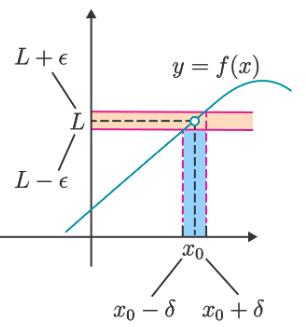
\includegraphics[width=6cm]{images/Epsilon_delta_definition.png}
\end{figure}
As $\epsilon$ becomes smaller and smaller, there always exists a $\delta$ that satisfies the property that for any $x$ in the open interval $(x_0-\delta,x_0+\delta)$, the value of $f(x)$ lies in the interval $(L-\epsilon, L+\epsilon)$.

\begin{exmp}{}{} 
Prove that \[ \lim_{x \to 3} 2x+4 = 10. \] \end{exmp}

Before the proof, we work backwards to find the value of $\delta$ in terms of $\epsilon$ and $x_0$, which we then declare in our proof.

$\forall \epsilon > 0$, $\exists \delta > 0$, $\forall x \in \RR$,
\[ |x-3| < \delta \implies |f(x)-10| < \epsilon \]
Let $\epsilon > 0$ be given.
\[ |f(x)-10| = |2x+4-10| = |2x-6| = 2|x-3| < \epsilon \]
Notice $|x-3| < \dfrac{\epsilon}{2}$. We can thus define $\delta \coloneqq \dfrac{\epsilon}{2}$. We now write our proof.

\begin{proof}
Let $\epsilon > 0$ be given. Choose $\delta = \dfrac{\epsilon}{2}$.

Then $\forall x \in \RR$, 
\begin{align*}
|x-3| &< \delta = \frac{\epsilon}{2} \\
2|x-3| &< \epsilon \\
|2x-6| &< \epsilon \\
|2x+4-10| &< \epsilon \\
|f(x)-10| &< \epsilon
\end{align*}
\end{proof}

\begin{exmp}{}{}
Use the formal definition of the limit to verify that 
\[ \lim_{x \to 3} \sqrt{2x+3} = 3. \]
\end{exmp}

We must prove that $\forall \epsilon > 0$, $\exists \delta > 0$ such that $\sqrt{2x+3} - 3 < \epsilon$ whenever $|x-3|<\delta$.
\begin{align*}
\sqrt{2x+3} - 3 &= \absolute{\frac{(2x+3)-3^2}{\sqrt{2x+3} + 3}} = \absolute{\frac{2x-6}{\sqrt{2x+3} + 3}} \\
&\le \absolute{\frac{2(x-3)}{3}} \\
&= \frac{2}{3} \absolute{x-3} < \frac{2}{3} \delta
\end{align*}
Hence, we can define 
\[ \epsilon \coloneqq \frac{2}{3} \delta \]
which we can use in our proof.
\pagebreak

\subsection{Important Limits}
\begin{equation}
\lim_{x \to 0} \frac{\sin x}{x} = 1
\end{equation}
\begin{proof}
This can be proven using the squeeze theorem, which will be discussed later.
\end{proof}

\begin{equation}
\lim_{x \to 0} \frac{1-\cos x}{x} = 0
\end{equation}
\begin{proof}
This can be proven using the squeeze theorem, which will be discussed later.
\end{proof}

\begin{equation}
\lim_{x\to 0} \frac{\arcsin x}{x} = 1
\end{equation}

\begin{equation}
\lim_{x\to \pm\infty} \brac{1+\frac{1}{x}}^x=e
\end{equation}
\pagebreak

\subsection{Continuity}
\begin{defn}{Continuity}{}
A function $f(x)$ is continuous at $x=a$ if 
\[ \lim_{x\to a} f(x)=f(a) \]
A function is said to be continuous on the interval  $[a,b]$ if it is continuous at each point in the interval.
\end{defn}
Note that this definition is also implicitly assuming that both $f(a)$ and $\lim_{x\to a}f(x)$ exist. If either of these do not exist the function will not be continuous at $x=a$.

This definition can be turned around into the following fact.
\begin{corollary}
If $f(x)$ is continuous at $x=a$ then
\[ \lim_{x \to a} f(x) = f(a) \quad \lim_{x \to a^-} f(x) = f(a) \quad \lim_{x \to a^+} f(x) = f(a) \]
\end{corollary}

A nice consequence of continuity is the following fact.
\begin{corollary}
If $f(x)$ is continuous at $x=b$ and $\lim_{x\to a}g(x)=b$ then
\[ \lim_{x \to a} f(g(x)) = f(\lim_{x \to a} g(x)) \]
\end{corollary}

\begin{exmp}{}{}
Evaluate the following limit:
\[ \lim_{x \to 0} e^{\sin x} \]
\end{exmp}

\begin{proof}[Solution]
Since we know that exponentials are continuous everywhere we can use the fact above.
\[ \lim_{x \to 0} e^{\sin x} = e^{\lim_{x \to 0} \sin x} = e^0 = \boxed{1} \]
\end{proof}

Another very nice consequence of continuity is the Intermediate Value Theorem.
\begin{thrm}{Intermediate Value Theorem}{}
Suppose that $f(x)$ is continuous on $[a,b]$ and let $M$ be any number between $f(a)$ and $f(b)$. Then there exists $c \in (a,b)$ such that $f(c)=M$.
\end{thrm}
All the Intermediate Value Theorem is really saying is that a continuous function will take on all values between $f(a)$ and $f(b)$.
\pagebreak

\section{Derivative}
\subsection{Definitions}
\begin{defn}{Derivative}{} 
The \vocab{derivative} of $f(x)$ with respect to $x$, denoted by $f^\prime(x)$, is defined as 
\begin{equation} f^\prime (x) = \lim_{h \to 0} \frac{f(x+h)-f(x)}{h}.
\end{equation}
\end{defn}

\begin{defn}{Differentiability}{} 
$f(x)$ is \vocab{differentiable} at $x_0$ if $f^\prime(x_0)$ exists. 

$f(x)$ is \vocab{differentiable} on an interval if the derivative exists for each and every point in the interval.
\end{defn}

\begin{defn}{Continuity}{} 
$f(x)$ is \vocab{continuous} at $x_0$ if $f(x)$ is differentiable at $x=x_0$.
\end{defn}

\begin{proof}
\begin{align*}
\lim_{x \to x_0} (f(x) - f(x_0)) &= \lim_{x \to x_0} \frac{(f(x) - f(x_0))(x-x_0)}{x - x_0}\\
&= \lim_{x \to x_0} \frac{f(x) - f(x_0)}{x - x_0} \cdot (x-x_0)\\
&= f^\prime (x_0) \cdot 0 = 0
\end{align*}
\end{proof}

\subsection{Theorems}
% move this to real analysis
\begin{thrm}{Extreme Value Theorem}{}
For a function $f$ continuous on $[a,b]$, it attains its maximum and minimum values on $[a,b]$.
\end{thrm}

\begin{proof}
We prove the case that $f$ attains its maximum value on $[a,b]$.

Since $f$ is continuous on $[a,b]$, we know it must be bounded on $[a,b]$ by the Boundedness Theorem. Let $M = \sup f$.

If there is some $c \in [a,b]$ where $f(c)=M$ there is nothing more to show -- $f$ attains its maximum on $[a,b]$.

Suppose otherwise, that there is no such $c$. Then $f(x)<M$ for all $x \in [a,b]$.

We define a new function $g$ by 
\[ g(x) = \frac{1}{M-f(x)}. \]

Note that $g(x)>0$ for every $x \in [a,b]$ and $g$ is continuous on $[a,b]$, and thus also bounded on this interval, again by the Boundedness theorem.

Given that $g$ is bounded on $[a,b]$, there must exist some $K>0$ such that $g(x) \le K$ for every $x \in [a,b]$.

Consequently,
\[ \frac{1}{M-f(x)} \le K \implies f(x) \le M - \frac{1}{K} \]
for every $x \in [a,b]$. This contradicts the assumption that $M$ is the least upper bound.

That leaves as the only possibility that there is some $c$ in $[a,b]$ where $f(c)=M$. That is to say, $f$ attains its maximum on $[a,b]$.

The proof that $f$ attains its minimum on the same interval is argued similarly and is left as an exercise for the reader.
\end{proof}

\begin{thrm}{Mean Value Theorem}{}
Let $f:[a,b]\to\RR$ be a continuous function on the closed interval $[a,b]$ and differentiable on the open interval $(a,b)$. Then there exists $c \in (a,b)$ such that 
\[ f^\prime(c)=\frac{f(b)-f(a)}{b-a}. \]
\end{thrm}

\begin{figure}[H]
    \centering
    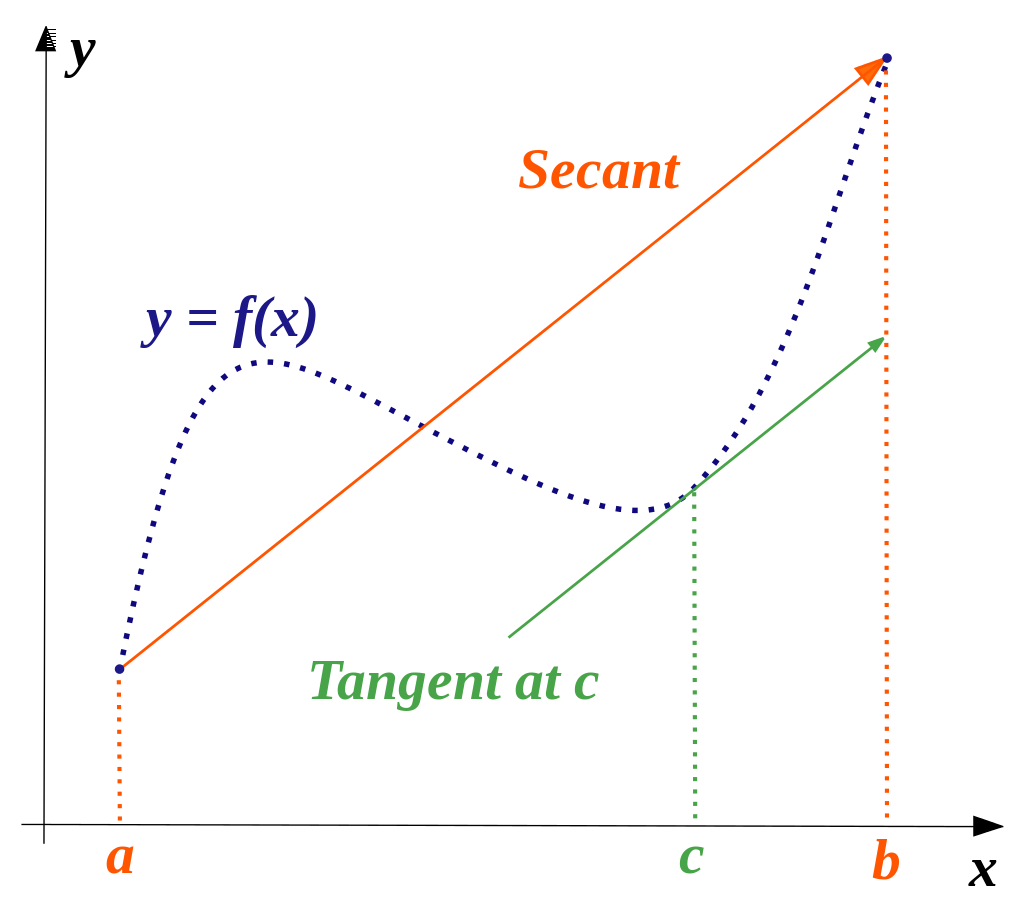
\includegraphics[width=8cm]{images/mean_value_thrm.png}
    \caption{Mean value theorem}
\end{figure}

\begin{thrm}{Rolle's Theorem}{}
Let $f:[a,b]\to\RR$ be a continuous function on the closed interval $[a,b]$ and differentiable on the open interval $(a,b)$, and $f(a)=f(b)$. Then there exists $c \in (a,b)$ such that 
\[ f^\prime(c)=0. \]
\end{thrm}
\begin{remark}
Rolle's Theorem is simply a special case of the Mean Value Theorem, where $f(a)=f(b)$.
\end{remark}

\subsection{Differentiation rules}
For a constant $c$ and functions $f$ and $g$, the following rules hold.

\begin{itemize}
\item \textbf{Scalar multiplication}
\[ (cf)^\prime = cf^\prime \]

\item \textbf{Addition rule}
\[ (f+g)^\prime = f^\prime + g^\prime \]

\begin{proof}
\begin{align*}
(f + g)^\prime (x) &= \lim_{h \to 0} \frac{(f+g)(x+h) - (f+g)(x)}{h}\\
&= \lim_{h \to 0} \frac{f(x+h) + g(x+h) - f(x) - g(x)}{h}\\
&= \lim_{h \to 0} \left[ \frac{f(x+h) - f(x)}{h} + \frac{g(x+h) - g(x)}{h} \right] \\
&= \lim_{h \to 0} \frac{f(x+h) - f(x)}{h} + \lim_{h \to 0} \frac{g(x+h) - g(x)}{h}\\
&= f^\prime (x) + g^\prime (x)
\end{align*}
\end{proof}

\item \textbf{Power rule}
\[ \dv{x} x^n = n x^{n-1} \]

\begin{proof}
Using implicit differentiation,
\begin{align*}
y &= x^n \\
\ln y &= \ln x^n \\
\ln y &= n \ln x \\
\frac{y^\prime}{y} &= n \frac{1}{x}
\end{align*}
\[ y^\prime = y \frac{n}{x} = x^n \brac{\frac{n}{x}} = n x^{n-1} \]
\end{proof}

\item \textbf{Product rule}
\[ (fg)^\prime = f^\prime g + f g^\prime \]

\begin{proof}
\begin{align*}
(fg)^\prime (x) &= \lim_{h \to 0} \frac{(fg)(x+h) - (fg)(x)}{h}\\
&= \lim_{h \to 0} \frac{f(x+h) g(x+h) - f(x) g(x)}{h}\\
&= \lim_{h \to 0} \frac{f(x+h) g(x) - f(x) g(x) + f(x+h) g(x+h) - f(x+h) g(x)}{h}\\
&= \lim_{h \to 0} \frac{f(x+h) g(x) - f(x) g(x)}{h} + \lim_{h \to 0} \frac{f(x+h) g(x+h) - f(x+h) g(x)}{h}\\
&= \lim_{h \to 0} \frac{f(x+h) - f(x)}{h}g(x) + \lim_{h \to 0} \frac{g(x+h) - g(x)}{h}f(x+h)\\
&= \left[\lim_{h \to 0} \frac{f(x+h) - f(x)}{h}\right] g(x) + \left[\lim_{h \to 0} \frac{g(x+h) - g(x)}{h}\right] f(x)\\
&= f^\prime (x) g(x) + f(x) g^\prime (x)
\end{align*}
\end{proof}

\item \textbf{Quotient rule}
\[ \brac{\frac{f}{g}}^\prime = \frac{f^\prime g - fg^\prime}{g^2} \] 

\begin{proof}
\begin{align*}
\left[\frac{f(x)}{g(x)}\right]^\prime &= \lim_{h \to 0} \frac{\frac{f(x+h)}{g(x+h)} - \frac{f(x)}{g(x)}}{h}\\
&= \lim_{h \to 0} \frac{1}{h} \frac{f(x+h) g(x) - f(x) g(x+h)}{g(x+h) g(x)}\\
&= \lim_{h \to 0} \frac{1}{h} \frac{f(x+h) g(x) - f(x) g(x) + f(x) g(x) - f(x) g(x+h)}{g(x+h) g(x)}\\
&= \lim_{h \to 0} \frac{1}{g(x+h) g(x)} \left[ \frac{f(x+h)g(x) - f(x)g(x)}{h} + \frac{f(x)g(x) - f(x)g(x+h)}{h} \right] \\
&= \lim_{h \to 0} \frac{1}{g(x+h) g(x)} \left[ g(x)\frac{f(x+h) - f(x)}{h} - f(x)\frac{g(x) + g(x+h)}{h} \right] \\
&= \frac{1}{g^2(x)} [g(x) f^\prime(x) - f(x) g^\prime(x)] \\
&= \frac{f^\prime(x) g(x) - f(x) g^\prime(x)}{g^2(x)}
\end{align*}
\end{proof}

\item \textbf{Chain rule}
\begin{thrm}{Chain rule}{} 
If $f$ and $g$ are both differentiable functions and we define $F(x) = (f \circ g)(x)$, then the derivative of $F(x)$ is
\begin{equation}
F^\prime (x) = f^\prime(g(x)) g^\prime(x) 
\end{equation} 
\end{thrm}
\begin{proof}

\end{proof}
\end{itemize}

\subsection{Implicit differentiation}
\textbf{Implicit differentiation} simply means differentiating both sides of the equation with respect to a variable.

\subsection{Taylor Series}
A function $f$ can be represented as a Taylor series about position $a$ if
\begin{itemize}
\item it is continuous near $a$ and
\item all of its derivatives are continuous near $a$
\end{itemize}

Using the notation $\Delta x = x-a$:
\[ f(x)=f(a)+\Delta xf^\prime(a)+\frac{\Delta x}{2!}f^{\prime\prime}(a) + \frac{\Delta x}{3!}f^{(3)}(a) + \cdots + \frac{\Delta x}{n!}f^{(n)}(a) + \cdots \]

If infinitely many terms are used, this approximation is exact near $a$.

If all terms of order $n$ and above are discarded then the error is approximately proportional to $\Delta x^n$ (assuming that $\Delta x$ is small). Then the approximation is said to be $n$-th order accurate. For example, a third order accurate approximation for $f(x)$ has error proportional to $\Delta x^3$. We say that  the error is of order $\Delta x^3$ or $O(\Delta x^3)$.
\[ f(x)=f(a)+\Delta xf^\prime(a)+\frac{\Delta x}{2!}f^{\prime\prime}(a) + O(\Delta x^3) \]


Maclaurin series,  determine radius and interval
of convergence of a power series

\subsection{Newton's Method}
In this section we are going to look at a method for approximating solutions to equations.

\begin{figure}[H]
    \centering
    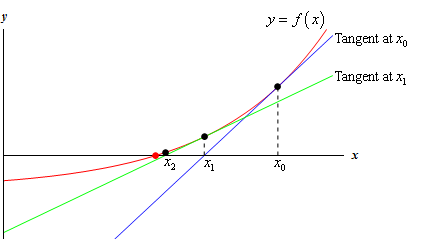
\includegraphics[width=10cm]{images/newton_method.png}
\end{figure}

Suppose that we want to approximate the solution to $f(x)=0$. Suppose that we have somehow found an initial rough approximation to the solution: $x=x_0$. The tangent line to $f(x)$ at $x=x_0$ is
\[ y = f(x_0) + f^\prime(x_0)(x-x_0) \]

This tangent line crosses the $x$-axis much closer to the actual solution to the equation than $x_0$ does. Let the tangent at $x_0$ intersect $x$-axis at $x_1$. We use this point as our new approximation to the solution. $x_1$ is given by:
\[ x_1 = x_0 - \frac{f(x_0)}{f^\prime(x_0)} \]

Repeat the process; form up the tangent line at $x_1$ and use its root $x_2$ as a new approximation:
\[ x_2 = x_1 - \frac{f(x_1)}{f^\prime(x_1)} \]

Here is the general Newton's Method:
\begin{thrm}{Newton's Method}{}
If $x_n$ is an approximation of a solution of $f(x)=0$ and if $f^\prime(x_n) \neq 0$, then the next approximation is given by
\[ x_{n+1} = x_n - \frac{f(x_n)}{f^\prime(x_n)} \]
\end{thrm}
\pagebreak

\section{Integral}
\subsection{Definition}
We use the \textbf{Riemann} definition of an integral:
\begin{defn}{Integral}{}
An integral is defined as an infinite sum over an interval.
\begin{equation}
\int_a^b f(x) \dd{x} = \lim_{n \to \infty} \sum_{i=1}^n f(x_i) \Delta x
\end{equation}
\end{defn}

A Riemann sum is an approximation of an integral by a finite sum.

Let $f$ be defined on the closed interval $[a,b]$ and let $\Delta x$ be a partition of $[a,b]$, with
\[ a=x_1 < x_2 < \cdots < x_n < x_{n+1}=b.\]

Let $\Delta x_i$ denote the length of the $i$th subinterval $[x_i,x_{i+1}]$ and let $c_i$ denote any value in the $i$th subinterval.

The sum
\[ \sum_{i=1}^n f(c_i)\Delta x_i\]
is a Riemann sum of $f$ on $[a,b]$.

As the subinterval becomes infinitesimally small, 
\begin{equation} \int _{a}^{b}f(x) \dd{x} = \lim _{\Delta x \to 0} \sum _{i=1}^{n} f(x_{i}) \Delta x_{i} \end{equation}

\begin{figure}[H]
	\centering
	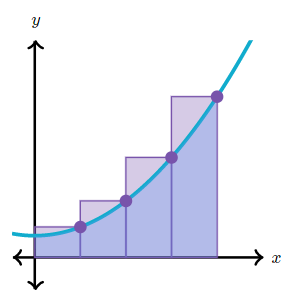
\includegraphics[width=8cm]{Riemanns_sums}
\end{figure}

Given a graph $y=f(x)$, and we want to find the integral on the $x$-interval $[0,1]$.

Split the interval $[0,1]$ into $n$ equal subintervals 
\[\sqbrac{0, \frac{1}{n}}, \sqbrac{\frac{1}{n}, \frac{2}{n}}, \cdots, \sqbrac{\frac{n-1}{n}, 1}.\]

Consider the height of the rectangles. We take the right value. Hence for the $k$th subinterval $\sqbrac{\dfrac{k-1}{n}, \dfrac{k}{n}}$ where $k=1,\dots,n$, height of rectangle is $f\brac{\dfrac{k}{n}}$.

Area of $k$th rectangle is \[ \frac{1}{n} \cdot f\brac{\frac{k}{n}}.\]
Therefore, the integral is obtained by summing up the area of $n$ rectangles, which gives us
\begin{equation} \int_{0}^{1} f(x) \dd{x} = \lim_{n \to \infty} \sum_{k=1}^{n} \frac{1}{n} f\brac{\frac{k}{n}} \end{equation}
where there are infinitely many rectangles, i.e. $n \to \infty$.

\begin{thrm}{Fundamental Theorem of Calculus}{}
The fundamental theorem of (single variable) calculus states that if $f^\prime$ is continuous on $[a,b]$, then the integral of the derivative across the bounds is equal to the original function at the bounds:
\begin{equation}
\int_a^b f^\prime(x) \dd{x} = f(b)-f(a)
\end{equation}
or equivalently,
\begin{equation}
\dv{x} \int_{a}^{x} f(s) \dd{s} = f(x)
\end{equation}
\end{thrm}

% https://www2.clarku.edu/faculty/djoyce/ma121/FTCproof.pdf

Using the definition of the derivative, we differentiate the following integral:
\begin{align*}
\dv{x} \int_{a}^{x} f(s) \dd{s} &= \lim_{h \to 0} \frac{\int_{a}^{x+h} f(s) \dd{s} - \int_{a}^{x} f(s) \dd{s}}{h}\\
&= \lim_{h \to 0} \frac{\int_{x}^{x+h} f(s) \dd{s}}{h}\\
&= \lim_{h \to 0} \frac{h f(x)}{h}\\
&= f(x)
\end{align*}
% https://math.libretexts.org/Bookshelves/Calculus/Calculus_3e_(Apex)/05%3A_Integration/5.04%3A_The_Fundamental_Theorem_of_Calculus

\subsection{Integration rules}
For constant $k\in\RR$ and functions $f(x)$ and $g(x)$, the following rules hold.
\begin{itemize}
\item \textbf{Sum and difference rule}
\[ \int f(x)\pm g(x) \dd{x} = \int f(x) \dd{x} \pm \int g(x) \dd{x} \]

\item \textbf{Scalar multiplication}
\[ \int kf(x) \dd{x} = k\int f(x) \dd{x} \]

\item \textbf{Power rule}
\[ \int x^n \dd{x} = \frac{x^{n+1}}{n+1} + C \]

\item \textbf{Constant rule}
\[ \int a\dd{x} = ax + C \]
\end{itemize}

\subsection{Integration techniques}
\subsubsection{Integrals of powers and of trigonometric functions}
Reciprocal rules:
\[ \int \frac{1}{x} \dd{x} = \ln|x| + C \]
\[ \int \frac{1}{ax+b} \dd{x} = \frac{1}{a} \ln(ax+b) + C \]

Exponential functions:
\[ \int e^x \dd{x} = e^x + C \]
\[ \int a^{x} \dd{x} = \frac{a^x}{\ln a} + C \]

Natural log rule:
\[ \int \ln x \dd{x} = x\ln x - x + C \]

Trigonometric functions:
\[ \int \sin x \dd{x} = -\cos x + C \]

\[ \int \cos x \dd{x} = \sin x + C \]

\[ \int \tan x \dd{x} = \ln|\sec x| + C \]

\[ \int \cosec x \dd{x} = \ln|\cosec x - \cot x| + C \]

\[ \int \cosec^2x \dd{x} = -\cot x + C \]

\[ \cosec x \cot x \dd{x} = -\cosec x + C \]

\[ \sec x \dd{x} = \ln|\sec x + \tan x| + C \]

\[ \int \sec^2 x \dd{x} = \tan x + C \]

\[ \int \sec x \tan x \dd{x} = \sec x + C \]

\[ \int \cot x \dd{x} = \ln|\sin x| + C \]

Inverse trigonometric functions:
\[ \int \frac{1}{\sqrt{1-x^2}} \dd{x} = \sin^{-1}x + C \]
\[ -\int \frac{1}{\sqrt{1-x^2}} \dd{x} = \cos^{-1}x + C \]
\[ \int \frac{x}{1+x^2} \dd{x} = \tan^{-1}x + C \]

\subsubsection{Substitution}
\begin{equation}
\int f(g(x)) g^\prime (x) \dd{x} = \int f(u) \dd{u}
\end{equation}
where $u=g(x)$.

The most common way of doing a integral by substitution, and the only way for indefinite integrals, is as follows:
\begin{enumerate}
\item Change variables from $x$ to $u$ (hence the common name ``$u$-substitution")
\item Keep track of the relation between $\dd{x}$ and $\dd{u}$
\item If you chose correctly you can now do the $u$-integral
\item When you are done, substitute back for $x$
\end{enumerate}

\begin{exmp}{}{}
Compute $\int\sin^nx\cos x\dd{x}$.
\end{exmp}
\begin{proof}[Solution]
Substitute $u = \sin x$ and $\dd{u} = \cos x \dd{x}$. This turns the integral into $\int u^n\dd{u}$ which is easily valuated as $u^{n+1}/(n+1)$. Now plug back in $u = \sin x$ and you get the answer
\[ \frac{\sin^{n+1}x}{n+1}. \]
\end{proof}

\begin{exmp}{}{}
Compute $\int_1^2\dfrac{x}{x^2+1}\dd{x}$.
\end{exmp}
\begin{proof}[Solution]
Let $u=x^2+1$ then $\dd{u} = 2x \dd{x}$, so the integrand becomes $(1/2)\dd{u}/u$. If $x$ goes
from 1 to 2 then $u$ goes from 2 to 5, thus the integral becomes
\[ \int_2^5\frac{1}{2}\frac{\dd{u}}{u} = \frac{1}{2}(\ln5-\ln2). \]
\end{proof}

\begin{exmp}{}{}
Compute $\int xe^{x^2}\dd{x}$.
\end{exmp}
\begin{proof}[Solution]
To do this integral we'll use the following substitution.
\[ u = x^2 \quad \dd{u} = 2x \quad \dd{x} \implies x \dd{x} = \frac{1}{2} \dd{u} \]
\[ \int x e^{x^2} \dd{x} = \frac{1}{2}\int e^u \dd{u} = \frac{1}{2}e^u + c = \frac{1}{2}e^{x^2} + c \]
\end{proof}



\subsubsection{Integration by parts}
From the product rule used for differentiation, we obtain
\begin{equation}
\int f g^\prime \dd{x} = fg - \int f^\prime g \dd{x}
\end{equation}
Alternatively, we can rewrite this as 
\begin{equation}
\int u \dd{v} = uv - \int v \dd{u}
\end{equation}

DI method

\subsubsection{Partial fraction decomposition}

\subsubsection{Trigonometric substitutions}
\begin{itemize}
\item Pythagorean identity: $\sin^2x + \cos^2x = 1$

\item Double-angle formulae

These can be used in the integrals of $\sin^2x$ and $\cos^2x$.

\item Product-to-sum identities
\end{itemize}

\subsubsection{Integrals of powers of trigonometric functions}

\subsubsection{Integrals of hyperbolic functions}

\subsubsection{Completing the square}

\subsubsection{Elimination of radicals by substitution}

\subsubsection{Weierstrass substitution}
Substituting the tangent of a half-angle: $t=\tan\dfrac{\theta}{2}$

Through trigonometric identities and manipulation, we have
\[ \sin\theta = \frac{2t}{1+t^2} \quad \cos\theta = \frac{1-t^2}{1+t^2} \quad \dd{\theta} = \frac{2\dd{t}}{1+t^2} \]

Some examples here: % https://math.unt.edu/integration-bee-examples

Useful info here:
% https://artofproblemsolving.com/community/c5h3108982p28119885
% https://www.quora.com/How-can-I-prepare-for-an-integration-bee
% https://tutorial.math.lamar.edu/pdf/calculus_cheat_sheet_integrals.pdf
% https://lehman.edu/faculty/rbettiol/old_teaching/110notes/notes04.pdf
% https://www2.math.upenn.edu/~rimmer/math104/ch8sc2notes.pdf
More info to be found on Youtube.

More problems here: % https://artofproblemsolving.com/community/c4h3164398_hmmt_integration_bee_mock_problems_2
\pagebreak

\subsubsection{Odd and even functions}
An odd function $f(x)$ satisfies $f(x)=-f(-x)$ for all $x$. Hence for any finite $a$,
\[ \int_{-a}^a f(x) \dd{x} = 0 \]

An even function $f(x)$ satisfies $f(x)=f(-x)$ for all $x$. Hence for any finite $a$,
\[ \int_{-a}^a f(x) \dd{x} = 2\int_0^a f(x) \dd{x} \]

\subsubsection{Reflections}
This is known as \textbf{King's property}, which states that we can revere the interval of integration: to ``integrate backwards".
\begin{equation}
\int_a^b f(x) \dd{x} = \int_a^b f(a+b-x) \dd{x}
\end{equation}
Instead of the function being centred at 0, the function is now centred at $\frac{a+b}{2}$. Then
\[ \int_a^b f(x) \dd{x} = \frac{1}{2} \int_a^b f(x) + f(a+b-x) \dd{x} \]

\subsubsection{Inversions}
Suppose the function $f$ has bounded anti-derivative on $[0,\infty]$. Then via the u-substitution $x\to\frac{1}{x}$,
\[ \int_0^\infty f(x) \dd{x} = \frac{1}{2}\int_0^\infty f(x) + \frac{f(\frac{1}{x})}{x^2} \dd{x} \]

\subsubsection{Inverse functions}
Suppose the function $f$ is one-to-one and increasing. Then a geometric equivalence may be established:


\subsubsection{Feynman's integration trick}
DIfferentiating under the integral sign

\subsection{Approximation of Integral}
\subsubsection{Trapezium rule}
We can sample the integrand at regular integrals and carry out an estimate based on this. One way of doing that is to approximate the function by a sequence of straight line segments. The area between each segment and the $x$-axis is a \emph{trapezium}, meaning that if the width of the interval is $h$, and the $y$-values at each end of the interval are $y_i$ and $y_{i+1}$, then the area of the trapezium is
\[ \frac{h}{2}(y_i+y_{i+1}). \]
The entire area between the curve and the $x$-axis, which is to say the integral, can be approximated by adding together several such trapezia. If there are n trapezia, and n+1 y-values (ordinates) running from $y_0$ to $y_n$, then the integral is approximately
\begin{equation}
T_n=\frac{h}{2}\,(y_0+2\,y_2+2\,y_2+\dots+2\,y_{n-2}+2\,y_{n-1}+y_n)
\end{equation}

\subsubsection{Simpson's Rule}
\vocab{Simpson's Rule} is based on the fact that given any three points, you can find the \emph{equation of a quadratic} through those points. 

This fact inspired Simpson to approximate integrals using quadratics, as follows.

If you want to integrate $f(x)$ over the interval $[a,b]$:
\begin{enumerate}
\item Find $f(a)$, $f(b)$ and $f(m)$ where $m=\dfrac{a+b}{2}$.
\item Find a quadratic $P(x)$ that goes through these three points.
\end{enumerate}

Since quadratics are easy to integrate, you simply need to integrate the quadratic over the interval. It turns out that the integral of the quadratic over the interval $[a,b]$ always comes out to 
\begin{equation}
\frac{b-a}{6}[f(a)+4f(m)+f(b)]
\end{equation}

For even $n$ subdivisions,
\begin{equation}
\int_a^bf(x)x' \approx \frac {\Delta x}{3} (f(x_0) + 4f(x_1) + 2f(x_2) + \cdots + 4f(x_{n-1} )+ f(x_n))
\end{equation}
where $\Delta x = \dfrac{b-a}{n}$, $x_i =a+ i\Delta x$.

\subsection{Parametric Equations and Polar Coordinates}

\pagebreak

\section{Ordinary Differential Equations}
% https://www.math.hkust.edu.hk/~machas/differential-equations.pdf
% Computation of ordinary differential equations - Euler's method and proof of convergence. Multistep methods, including order, the root condition and the concept of convergence. Runge-Kutta schemes. Stiff equations and A-stability.

\begin{defn}{Ordinary differential equation}{} 
An ordinary differential equation (ODE) is an equation relating a variable, say $x$, a function, say $y$, of the variable $x$, and finitely many of the derivatives of $y$ with respect to $x$.

That is, an ODE can be written in the form
\[ f\brac{x,y,\dv{y}{x},\dv[2]{y}{x},\cdots,\dv[k]{y}{x}} = 0 \]
for some function $f$ and some natural number $k$. Here $x$ is the \textbf{independent variable} and the ODE governs how the \textbf{dependent variable} $y$ varies with $x$. 
\end{defn}

\begin{remark}
The equation may have no, one or many functions $y(x)$ which satisfy it; the problem is usually to find the most general solution $y(x)$, a function which satisfies the differential equation.
\end{remark}

The derivative $\dv[k]{y}{x}$ is said to be of order $k$. We say that an ODE has \textbf{order} $k$ if it involves derivatives of order $k$ and less. Hence, a first-order differential equation involves up to the first derivative $\dv{y}{x}$, whereas a second-order differential equation involves up to the second derivative $\dv[2]{y}{x}$.

\subsection{First-order differential equations}
\vocab{First-order differential equations} take the form
\[ \dv{y}{x} = f(x,y) \]
There are several standard methods for solving first order ODEs and we look at some of these now.

\subsubsection{Direct integration}
If the ODE takes the form
\[ \dv{y}{x} = f(x) \]
in other words the derivative is a function of $x$ only, then we can integrate directly.

\begin{exmp}{}{}
Find the general solution of
\[ \dv{y}{x} = x^2\sin x \]
\end{exmp}

\begin{proof}[Solution]
By direct integration,
\[ y = \int x^2\sin x \dd{x} = (2-x^2) \cos x + 2x \sin x + c \]
which is done using integration by parts.
\end{proof}

\subsubsection{Separation of variables}
This method is applicable when the first order ODE takes the form
\[ \dv{y}{x} = a(x)b(y) \]
where $a$ is a function of $x$ and $b$ is a function of $y$. 

Such an equation is called \textbf{separable}. These equations can be rearranged and solved as follows. First
\[ \frac{1}{b(y)}\dv{y}{x} = a(x) \]
and then integrating with respect to $x$ we find
\[ \int \frac{1}{b(y)} \dd{y} = \int a(x) \dd{x} \]
Here we have assumed that $b(y) \neq 0$; if $b(y) = 0$ then the solution is $y = c$ where $c$ is a constant.

\begin{exmp}{}{}
Find the general solution to the separable differential equation
\[ x(y^2-1) + y(x^2-1)\dv{y}{x} = 0 \]
where $0<x<1$.
\end{exmp}

\begin{proof}[Solution]
We rearrange to obtain
\[ \frac{y}{y^2-1}\dv{y}{x} = -\frac{x}{x^2-1} \]
After integration we obtain
\[ \frac{1}{2}\ln|y^2-1| = -\frac{1}{2}\ln|x^2-1| + c \]
where $c$ is a constant. This can be arranged to give
\[ (x^2-1)(y^2-1) = c. \]
Note that the constant functions $y=1$ and $y=-1$ are also solutions of the differential equation, but are already included in the given general solution, for $c=0$.
\end{proof}

\subsubsection{Reduction to separable form by substitution}
Some first order differential equations can be transformed by a suitable substitution into separable form.

\begin{exmp}{}{}
Find the general solution of
\[ \dv{y}{x} = \sin(x+y+1) \]
\end{exmp}

\begin{proof}[Solution]
Let $u(x) = x + y(x) + 1$ so that $\dv{u}{x} = 1 + \dv{y}{x}$. Then the original equation can be written as $\dv{u}{x} = 1 + \sin u$, which is separable. We have
\[ \frac{1}{1+\sin u}\dv{u}{x} = 1 \]
which integrates to
\[ \int \frac{1}{1+\sin u} \dd{u} = x+c \]
Let us evaluate the integral on the left hand side:
\begin{align*}
\int \frac{1}{1+\sin u} \dd{u}
&= \int \frac{1-\sin u}{(1+\sin u)(1-\sin u)} \dd{u} \\
&= \int \frac{1-\sin u}{1-\sin^2u} \dd{u} = \int \frac{1-\sin u}{\cos^2u} \dd{u} \\
&= \int \frac{1}{\cos^2u} \dd{u} - \int \frac{\sin u}{\cos^2u} \dd{u} \\
&= \tan u - \frac{1}{\cos u} + c
\end{align*}
Therefore 
\[ \tan u - \frac{1}{\cos u} = x+c \]
In terms of $x$ and $y$, the solution is given by
\[ \tan (x+y+1) - \frac{1}{\cos (x+y+1)} = x+c \]
or
\[ \sin (x+y+1) - 1 = (x+c) \cos (x+y+1). \]
This solution, where we have not found $y$ in terms of $x$, is called an \textbf{implicit solution}.
\end{proof}

A special group of first order differential equations is those of the form
\[ \dv{y}{x} = f\brac{\frac{y}{x}} \]
These differential equations are called \textbf{homogeneous} and they can be solved with a substitution
of the form
\[ y(x) = xv(x) \]
to get a new equation in terms of x and the new dependent variable $v$. This new equation will be
separable:
\[ \dv{y}{x} = v + x\dv{v}{x} \]
which becomes
\[ x\dv{v}{x} = f(v) - v \]

\subsection{First-order differential equations}
In general, a $k$-th order \textbf{inhomogeneous linear ODE} takes the form
\[ a_k(x)\dv[k]{y}{x} + a_{k-1}(x)\dv[k-1]{y}{x} + \cdots + a_1(x)\dv{y}{x} + a_0(x)y = f(x) \]
where $a_k(x) \neq 0$. The equation is \textbf{homogeneous} if $f(x) = 0$. 

\subsubsection{First-order linear ODEs}
Looking specifically at first order linear ODEs, which take the general form
\[ \dv{y}{x} + P(x)y = Q(x) \]
we see that the homogeneous form, that is when $Q(x) = 0$, is separable. On the other hand, the inhomogeneous form can be solved using an \textbf{integrating factor} $I(x)$ given by
\[ I(x) = e^{\int P(x) \dd{x}} \]
\begin{proof}
Simply multiply the general equation for first-order linear ODEs through by the integrating factor to obtain
\[ e^{\int P(x) \dd{x}} \dv{y}{x} + P(x) e^{\int P(x) \dd{x}}y = e^{\int P(x) \dd{x}} Q(x) \]
Using the product rule for derivatives, we see that this gives
\[ \dv{}{x}\brac{e^{\int P(x) \dd{x}}y} = e^{\int P(x) \dd{x}} Q(x) \]
and we can now integrate directly and rearrange, to obtain
\[ y = e^{-\int P(x) \dd{x}} \sqbrac{\int e^{\int P(x)dx} Q(x) \dd{x} + c}. \]
\end{proof}

\begin{exmp}{}{}
Solve the linear differential equation 
\[ \dv{y}{x} + 2xy = 2xe^{-x^2}. \]
\end{exmp}
\begin{solution}
We can easily see that the given differential equation is in the form of a first-order linear ODE.

First we find the integrating factor:
\[ I(x) = e^{\int 2x \dd{x}} = e^{x^2} \]

Multiplying the given differential equation through by the integrating factor this gives
\[ e^{x^2} \dv{y}{x} + 2xe^{x^2}y = 2x \]
that is
\[ \dv{}{x}\brac{e^{x^2}y}= 2x \]
Integrating this gives us
\[ e^{x^2}y = x^2 + c \]
so the general solution is $y = (x^2+c)e^{-x^2}$.
\end{solution}

%Euler's method in finding a numerical solution

\subsection{Second-order differential equations}
The main subject of this section is linear ODEs with constant coefficients, but before we look at these we give two theorems that are valid in the more general case.

\subsubsection{Two theorems}


\subsubsection{Second-order homogeneous linear ODEs}

\pagebreak

\section{Laplace transform}
\begin{defn}{Laplace transform}{}
The Laplace transform of a signal (function) $f$ is the function $F = \mathcal{L}(f)$ defined by
\begin{equation}
F(s) = \int_0^\infty f(t)e^{-st} \dd{t}
\end{equation}
for those $s \in \CC$ for which the integral makes sense.
\end{defn}

\begin{remark}
$F$ is a complex-valued function of complex numbers. $s$ is called the (complex) frequency variable, with units \unit{sec^{-1}}; $t$ is called the time variable (in \unit{sec}); $st$ is unitless. For now, we assume $f$ contains no impulses at $t = 0$.
\end{remark}

\begin{notation}
Lowercase letter denotes signal; uppercase letter denotes its Laplace transform; for example, $U$ denotes $\mathcal{L}(u)$, $V_\text{in}$ denotes $\mathcal{L}(v_\text{in})$.
\end{notation}

% https://web.stanford.edu/~boyd/ee102/laplace.pdf

\chapter{Multivariable Calculus}
\section{Introduction}
\subsection{Vectors}
From the Cartesian product in Set Theory, we know that
\[ \RR^n = (x_1, x_2, \dots, x_n) \]
which is the set of all $n$-tuples of real numbers $x$.

The elements of $\RR^n$ are the points in $n$-dimensional space and are also called $n-$dimensional vectors.

Vector operations
\begin{itemize}
\item Scalar multiplication

Given a vector $x = (x_1, \dots, x_n)$ in $\RR^n$ and a scalar $\alpha \in \RR$, the product is the vector 
\[ \alpha x = (\alpha x_1, \dots, \alpha x_n). \]

\item Addition and subtraction

Another vector $y = (y_1, \dots, y_n)$ can to added to $x$ to give a vector
\[ x+y = (x_1+y_1, \dots, x_n+y_n). \]
Similarly, we can also subtract vectors defining $x-y=x+(-1)y$ and then
\[ x-y = (x_1-y1, \dots, x_n-y_n). \]

\begin{remark}
Because elements of $\RR^n$ can be multiplied by a scalar and added, $\RR^n$ is a vector space.
\end{remark}

\item Magnitude

A vector $x = (x_1, \dots, x_n)$ has a magnitude (length) of
\[ |x| = \sqrt{x_1^2+\cdots+x_n^n} \]

Since $x-y$ goes from point $y$ to point $x$, the length of this vector is the distance between the points:
\[ |x-y| = \sqrt{(x_1-y_1)^2+\cdots+(x_n-y_n)^2} \]

\item Dot product

The dot product of vectors $x$ and $y$ in $\RR^n$ is a scalar given by
\[ x \cdot y = x_1y_1 + x_2y_2 + \cdots + x_ny_n. \]
Then we have the following corollary:
\[ x \cdot x = |x|^2 \]

\end{itemize}

\subsection{Functions of several variables}
We are interested in functions $f$ from $\RR^n$ to $\RR^m$ (or more generally from a subset $D \subset \RR^n$ to $\RR^m$ called the domain of the function). A function $f$ assigns to each $x \in \RR^n$ a point $y \in \RR^m$ and we write
\[ y=f(x) \]
The set of all such points $y$ is the range of the function.

Each component of $y = (y_1, \dots, y_m)$ is real-valued function of $x \in \RR^n$ written $y_i = f_i(x)$ and the function can also be written as the collection of $n$ functions
\[ y_1 = f_1(x), \dots, y_m = f_m(x) \]
If we also write out the components of $x = (x_1, \dots, x_n)$, then are function can be written as $m$ functions of $n$ variables each:
\[ \begin{split}
y_1 &= f_1(x_1, \dots, x_n) \\
y_2 &= f_2(x_1, \dots, x_n) \\
&\vdots \\
y_m &= f_m(x_1, \dots, x_n)
\end{split} \]

The graph of the function is all pairs $(x,y)$ with $y=f(x)$. It is a subset of $\RR^{n+m}$.

Here are some special cases that are of particular interest.
\begin{enumerate}
\item $n = 1, m = 2$ (or $m = 3$). The function has the form
\[ y_1 = f_1(x), y_2 = f_2(x) \]
In this case the range of the function is a curve in $\RR^2$.

\item $n = 2, m = 1$. Then function has the form
\[ y = f(x_1, x_2) \]
The graph of the function is a surface in $\RR^3$.

\item $n = 2, m = 3$. The function has the form
\[ \begin{split}
y_1 &= f_1(x_1, x_2) \\
y_2 &= f_2(x_1, x_2) \\
y_3 &= f_3(x_1, x_2)
\end{split} \]
The range of the function is a surface in $\RR^3$.

\item $n = 3, m = 3$. The function has the form
\[ \begin{split}
y_1 &= f_1(x_1, x_2, x_3) \\
y_2 &= f_2(x_1, x_2, x_3) \\
y_3 &= f_3(x_1, x_2, x_3)
\end{split} \]
The function assigns a vector to each point in space and is called a \textbf{vector field}.
\end{enumerate}

\subsection{Limits}
Consider a function $y = f(x)$ from $\RR^n$ to $\RR^m$ (or possibly a subset of $\RR^n$). Let $x_0 = (x_{01},\dots,x_{0n})$ be a point in $\RR^n$ and let $y_0 = (y_{01},\dots,y_{0m})$ be a point in $\RR^m$. We say that $y_0$ is the limit of $f$ as $x$ goes to $x_0$, written
\begin{equation}
\lim_{x\to x_0} f(x) = y_0
\end{equation}
if for every $\epsilon > 0$ there exists a $\delta > 0$ so that if $|x-x_0|<\delta$ then $|f(x)-y_0|<\epsilon$. The function is continuous at $x_0$ if
\begin{equation}
\lim_{x\to x_0} f(x) = f(x_0)
\end{equation}
The function is continuous if it is continuous at every point in its domain.
\pagebreak

\section{Partial Derivatives}
\subsection{Limits}
We take the limit of the function $f(x,y)$ as $x$ approaches $a$ and as $y$ approaches $b$. This is denoted by
\[ \lim_{(x,y)\to(a,b)}f(x,y) \]

\begin{defn}{Continuity}{}
A function $f(x,y)$ is continuous at the point $(a,b)$ if
\[ \lim_{(x,y)\to(a,b)} f(x,y) = f(a,b) \]
\end{defn}

\subsection{What it is}
\begin{defn}{Partial derivative}{}
Suppose $f$ is a function from $\RR^2$ to $\RR$, given by $z=f(x,y)$. The \vocab{partial derivative} of $f$ with respect to $x$ at $(x_0,y_0)$ is defined as
\begin{equation}
f_x(x_0,y_0) = \lim_{h \to 0}\frac{f(x_0+h,y_0)-f(x_0,y_0)}{h}
\end{equation}
if the limit exists.

Similarly, the partial derivative of $f$ with respect to $y$ at $(x_0,y_0)$ is defined as
\begin{equation}
f_y(x_0,y_0) = \lim_{h \to 0}\frac{f(x_0,y_0+h)-f(x_0,y_0)}{h}.
\end{equation}
\end{defn}

\begin{notation}
We also use the notation
\[ f_x=\pdv{f}{x} \quad \text{and} \quad f_y=\pdv{f}{y}. \]
\end{notation}

\begin{notation}
We can also take second partial derivatives, given by
\[ \begin{split}
f_{xx} &= \pdv{}{x}\brac{\pdv{f}{x}} = \pdv[order={2}]{f}{x} \\
f_{yy} &= \pdv{}{y}\brac{\pdv{f}{y}} = \pdv[order={2}]{f}{y} \\
f_{xy} &= \pdv{}{y}\brac{\pdv{f}{x}} = \pdv{f}{x,y} \\
f_{yx} &= \pdv{}{x}\brac{\pdv{f}{y}} = \pdv{f}{y,x}
\end{split} \]
\end{notation}

\subsection{How to Do Partial Derivatives}
Keep in mind that we only need to find the derivative of functions with respect to one variable by keeping the rest of the variables constant.

\begin{exmp}{First partial derivative}{}
Find the partial derivative of $f(x,y)=2x^2-4xy+y^2$ with respect to $x$.
\end{exmp}
\begin{solution}
\begin{align*}
\pdv{f}{x}
&= \pdv{}{x}(2x^2-4xy+y^2) \\
&= 2(2x) - 4(1)y + 0\\
&= 4x - 4y 
\end{align*}
\end{solution}

\begin{exmp}{Second partial derivative}{}
Given that $f(x,y)=12x^2y-3xy^2$, find $f_{yx}$.
\end{exmp}
\begin{solution}
\begin{align*}
\pdv{f}{x,y}
&= \pdv{}{x} \brac{\pdv{f}{y}} \\
&= \pdv{}{x} \sqbrac{\pdv{}{y} (12x^2y - 3xy^2)} \\
&= \pdv{}{x}[12x^2(1) - 3x(2y)]\\
&= \pdv{}{x}(12x^2-6xy) \\
&= 12(2x)-6y(1) \\
&= 24x-6y
\end{align*}
\end{solution}

\begin{thrm}{}{}
If $f_x$, $f_y$, $f_{xy}$, $f_{yx}$ exist and are continuous near $(x_0, y_0)$, then
\[ f_{xy}(x_0, y_0) = fyx(x_0, y_0) \]
\end{thrm}

\subsection{Directional Derivatives}
To this point we've only looked at the two partial derivatives $f_x(x,y)$ and $f_y(x,y)$. Recall that these derivatives represent the rate of change of $f$ as we vary x (holding $y$ fixed) and as we vary $y$ (holding $x$ fixed) respectively. 

We now discuss how to find the rate of change of $f$ if we allow both $x$ and $y$ to change simultaneously. The problem here is that there are many ways to allow both $x$ and $y$ to change. For instance, one could be changing faster than the other and then there is also the issue of whether or not each is increasing or decreasing. So, before we get into finding the rate of change we need to get a couple of preliminary ideas taken care of first. The main idea that we need to look at is just how are we going to define the changing of $x$ and/or $y$.

Let's start off by supposing that we wanted the rate of change of $f$ at a particular point, say $(x_0,y_0)$. Let's also suppose that both $x$ and $y$ are increasing and that, in this case, $x$ is increasing twice as fast as $y$ is increasing. So as $y$ increases one unit of measure, $x$ increases two units of measure.

Let's suppose that a particle is sitting at $(x_0,y_0)$ and the particle will move in the direction given by the changing 
$x$ and $y$. At this point, the particle can be said to be moving in the direction
\[ \vec{v} = \langle {2,1} \rangle \]

There is still a small problem with this however. There are many vectors that point in the same direction. For instance, all of the following vectors point in the same direction as $\vec v = \langle {2,1} \rangle$:
\[ \vec{v} = \left\langle {\frac{1}{5},\frac{1}{10}}\right\rangle \quad \vec{v} = \langle {6,3}\rangle \quad \vec{v} = \left\langle {\frac{2}{\sqrt{5}},\frac{1}{\sqrt{5}}}\right\rangle \]

We need a way to consistently find the rate of change of a function in a given direction. We will do this by insisting that the vector that defines the direction of change be a unit vector. This means that for the example that we started off thinking about we would want to use
\[ \vec{v} = \left\langle {\frac{2}{\sqrt{5}},\frac{1}{\sqrt{5}}}\right\rangle \]

\begin{defn}{Directional derivative}{}
Rate of change of $f(x,y)$ in the direction of the unit vector $\vec{u}=\langle{a,b}\rangle$ is called the directional derivative and is denoted by $D_{\vec{u}} f(x,y)$.

The definition of the directional derivative is
\begin{equation}
{D_{\vec u}}f(x,y) = \lim_{h\to0} \frac{f(x + ah,y + bh) - f(x,y)}{h}
\end{equation}
\end{defn}

To derive an equivalent formula for taking directional derivatives, we define a new function of a single variable
\[ g(z) = f(x_0+az,y_0+bz) \]
where $x_0$, $y_0$, $a$, $b$ are some fixed numbers. Note that this really is a function of a single variable $z$.

Then by the definition of the derivative for functions of a single variable we have
\[ g^\prime(z) = \lim_{h\to0} \frac{g(z+h)-g(z)}{h} \]
and the derivative at $z=0$ is given by
\[ g^\prime(0) = \lim_{h\to0} \frac{g(h)-g(0)}{h} \]
If we now substitute in for $g(z)$ we get
\[ g^\prime(0) = \lim_{h\to0} \frac{g(h)-g(0)}{h} = \lim_{h\to0} \frac{f(x_0+ah,y_0+bh) - f(x_0,y_0)}{h} = D_{\vec u}f(x_0,y_0) \]
This gives us
\begin{equation}\tag{1}
g^\prime(0) = D_{\vec u}f(x_0,y_0)
\end{equation}

Now, let's look at this from another perspective. Let's rewrite $g(z)$ as $g(z) = f(x,y)$ where $x=x_0+az$ and $y=y_0+bz$. Applying chain rule,
\[ g^\prime(z) = \odv{g}{z} = \pdv{f}{x}\odv{x}{z} + \pdv{f}{y}\odv{y}{z} = f_x (x,y)a + f_y (x,y)b \]
This gives us
\[ g^\prime(z) = f_x (x,y)a + f_y (x,y)b \]
If we take $z=0$ we get $x=x_0$ and $y=y_0$. Plugging these into the above equation gives
\begin{equation}\tag{2}
g^\prime(0) = f_x (x_0,y_0)a + f_y (x_0,y_0)b
\end{equation}
Equating (1) and (2) gives
\[ {D_{\vec u}}f(x_0,y_0) = f_x(x_0,y_0)a + f_y(x_0,y_0)b \]
Allowing $x$ and $y$ to be any number we get the following formula for computing directional derivatives:
\[ {D_{\vec u}}f(x,y) = f_x(x,y)a + f_y(x,y)b \]
For three variables, directional derivative of $f(x,y,z)$ in the direction of the unit vector $\vec{u}=\langle{a,b,c}\rangle$ is given by
\begin{equation}
{D_{\vec u}}f(x,y,z) = f_x (x,y,z)a + f_y (x,y,z)b + f_z (x,y,z)c
\end{equation}

We can write the directional derivative as a \textbf{dot product} and notice that the second vector is nothing more than the unit vector $\vec u$ that gives the direction of change.
\begin{equation}
{D_{\vec u}} f(x,y,z) = \langle {f_x,f_y,f_z} \rangle \cdot \langle {a,b,c} \rangle
\end{equation}

Now let's give a name and notation to the first vector in the dot product since this vector will show up fairly regularly.
\begin{defn}{Gradient vector}
The gradient vector of $f$ is defined to be
\begin{equation}
\nabla f = \langle f_x,f_y,f_z \rangle
\end{equation}
\end{defn}

With the definition of the gradient we can now say that the directional derivative is given by
\[ {D_{\vec u}}f = \nabla f\cdot \vec u \]

\begin{thrm}{}{}
Maximum value of $D_{\vec u} f(\vec{x})$ (and hence then the maximum rate of change of the function $f(\vec{x})$) is given by $\left\|\nabla f(\vec{x})\right\|$ and will occur in the direction given by $\nabla f(\vec{x})$.
\end{thrm}

\begin{proof}

\end{proof}
\pagebreak

\section{Partial differential equations}
%https://www.youtube.com/watch?v=Ef3CNDTAuBM&list=PLdgVBOaXkb9Ab7UM8sCfQWgdbzxkXTNVD&index=5
\subsection{Definitions and Terminology}
\begin{defn}{Partial differential equation}{}
An equation involving a function and/or its partial derivatives. 
\end{defn}

For example, \[ \pdv{f}{t}=\pdv[order={2}]{f}{x} \]
where $f(x,t)$ is a function of multiple variables.

We can classify PDEs based on:
\begin{itemize}
\item \textbf{Order.}

The order is the number corresponding to the order of the highest partial derivative in the equation. 

For instance, the order of the following PDE is 2. 
\[ \pdv[order={2}]{f}{x}=\pdv{f}{t} \]

This also applies to mixed partial derivatives. For instance, the order of the following PDE is 3.
\[ \pdv[order={2,1}]{f}{x,y}=\pdv{f}{t} \]

\item \textbf{Number of independent variables.}

An independent variable is what we differentiate with respect to. 

\item \textbf{Linearity.}

A linear PDE is one in which the \emph{dependent} variable (the one being differentiated) appears only in a linear fashion.

For instance, the two PDEs above are linear as the partial derivatives are not being raised to a power or multiplied with each other.

The following PDE is non-linear.
\[ f\pdv[order={2}]{f}{x}=\pdv{f}{t} \]

\item \textbf{Homogeneity.}

A homogenous PDE is one in which every term only involves the dependent variable and/or its derivatives.

The first two PDEs above are homogenous as every term contains $f$ or its derivatives.

The following PDE is non-homogenous as there are two terms that do not contain $f$.
\[ \pdv[order={2}]{f}{x}=\pdv{f}{t}+x^2+\tan t \]

\item \textbf{Coefficient type.}

The coefficient here refers to the coefficient of the term involving the dependent variable and its derivatives. It can be either constant or variable.

For instance, the coefficients of the terms in the first two examples are 1. We say that these two PDEs have constant coefficients.

The following PDE has variable coefficients.
\[ \tan x\pdv[order={2}]{f}{x}=\pdv{f}{t} \]

\item \textbf{Parabolic, Hyperbolic, or Elliptic.}

We can do this classification for linear 2nd order PDEs which take the form of 
\[ A\pdv[order={2}]{f}{x} + B\pdv{f}{x,y} + C\pdv[order={2}]{f}{y} + D\pdv{f}{x} + E\pdv{f}{y} + Ff = G \]
where the coefficients are generally functions of $x$ or $y$.

For a \textbf{hyperbolic} PDE, $B^2-4AC>0$. Using variable substitutions to change $x$ and $y$ to $\eta$ and $\epsilon$ respectively, we can reduce the PDE to \[ \pdv[order={2}]{f}{\eta} - \pdv[order={2}]{f}{\epsilon} + g = 0 \] where $g$ denotes the first and lower order terms. This is similar to the equation of a hyperbola: $x^2-y^2=1$.

For a \textbf{parabolic} PDE, $B^2-4AC=0$. Using variable substitutions, we can reduce the PDE to \[ \pdv[order={2}]{f}{\eta} + g = 0. \] This is similar to the equation of a parabola: $x^2+y=0$.

For an \textbf{elliptic} PDE, $B^2-4AC<0$. Using variable substitutions, we can reduce the PDE to \[ \pdv[order={2}]{f}{\eta} + \pdv[order={2}]{f}{\epsilon} + g = 0. \] This is similar to the equation of an ellipse: $x^2+y^2=1$.

Note that if the coefficients are constants, the PDE can be hyperbolic, parabolic or elliptic. However, if the coefficients are variables, then it is possible for the PDE to be hyperbolic in some regions, and elliptic or parabolic in some regions.
\end{itemize}

\subsection{Solutions and Auxiliary Conditions}
There are a lot of solutions to a given PDE, hence it is important for us to know the auxiliary conditions, i.e. boundary and initial conditions, which dictate which technique we use to solve the PDE.
\begin{itemize}
\item A boundary condition expresses the behavior of a function on the boundary (border) of its area of definition. An initial condition is like a boundary condition, but then for the time-direction.
\end{itemize}

\section{Double integrals}
We want to integrate a function of two variables, $f(x,y)$. With functions of one variable we integrated over an \emph{interval} (i.e. a one-dimensional space) and so it makes some sense then that when integrating a function of two variables we will integrate over a \emph{region} of $\RR^2$ (two-dimensional space). 

We will start out by assuming that the region in $\RR^2$ is a rectangle which we will denote as follows,
\[ R=[a,b]\times[c,d] \]

This means that the ranges for $x$ and $y$ are $a \le x \le b$ and $c \le y \le d$.

% https://tutorial.math.lamar.edu/classes/calciii/DoubleIntegrals.aspx
\pagebreak

\section{Line integrals}
\subsection{Vector fields}
A vector field is basically what you get when associating each point in space with a vector.

\begin{defn}{Vector field}{}
A \vocab{vector field} in $\RR^n$ is a function $F : \RR^n \to  \RR^n$ that assigns to each $x \in \RR^n$ a vector $F(x)$. A vector field in $\RR^n$ with domain $U \subset \RR^n$ is called a vector field on $U$.
\end{defn}

The standard notation for the function $\vec{F}$ is:
\begin{align*}
\vec{F}(x,y) &= P(x,y)\hat{i} + Q(x,y)\hat{j} \\
\vec{F}(x,y,z) &= P(x,y,z)\hat{i} + Q(x,y,z)\hat{j} + R(x,y,z)\hat{k}
\end{align*}
depending on whether or not we're in two or three dimensions. The functions $P$, $Q$, $R$ are called \textbf{scalar functions}.

\begin{exmp}{}{}
Sketch the following vector field:
\[ \vec{F}(x,y) = -y\hat{i} + x\hat{j} \]
\end{exmp}
\begin{proof}[Solution]
To graph the vector field we need to get some ``values" of the function. This means plugging in some points into the function. Here are a couple of evaluations:
\begin{align*}
\vec{F}\brac{{\frac{1}{2},\frac{1}{2}}} &=  -\frac{1}{2}\hat{i} + \frac{1}{2}\hat{j} \\
\vec{F}\brac{{\frac{1}{2},-\frac{1}{2}}} &=  -\brac{{-\frac{1}{2}}}\hat{i} + \frac{1}{2}\hat{j} = \frac{1}{2}\hat{i} + \frac{1}{2}\hat{j} \\
\vec{F}\brac{{\frac{3}{2},\frac{1}{4}}} &=  -\frac{1}{4}\hat{i} + \frac{3}{2}\hat{j}
\end{align*}
So what do these evaluations tell us? The first one tells us that at the point $\brac{\dfrac{1}{2},\dfrac{1}{2}}$ we plot the vector $-\frac{1}{2}\hat{i} + \frac{1}{2}\hat{j}$.

Plotting points gives us the following sketch of the vector field:

\begin{figure}[H]
    \centering
    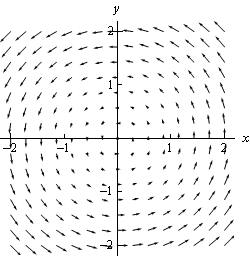
\includegraphics[width=8cm]{images/vec_field2.png}
\end{figure}
\end{proof}

\begin{defn}{Gradient vector}{}
Given a function $f(x,y,z)$, the gradient vector is defined by
\begin{equation}
\nabla f = \left\langle {{f_x},{f_y},{f_z}} \right\rangle
\end{equation}
This is a vector field and is often called a gradient vector field.
\end{defn}

\subsection{Types of line integrals}

\subsection{Fundamental Theorem for Line Integrals}
\begin{thrm}{Fundamental Theorem of Line Integrals}{}
Suppose that $C$ is a smooth curve from points $A$ to $B$ parameterised by $\vb{r}(t)$ for $t\in[a,b]$. Let $f$ be a differentiable function whose domain includes $C$ and whose gradient vector $\nabla f$ is continuous on $C$. Then
\begin{equation}
\int_C \nabla f \dd{\vb{r}} = f(\vb{r}(b)) - f(\vb{r}(a)) = f(B) - f(A)
\end{equation}
\end{thrm}
\begin{remark}
Similar to the fundamental theorem of calculus, the primary change is that gradient $\nabla f$ takes the place of the derivative $f^\prime$.
\end{remark}
% https://www.math.uci.edu/~ndonalds/math2e/16-3fundthm.pdf
% https://www.youtube.com/watch?v=_60sKaoRmhU

\subsection{Conservative Vector Fields}

\subsection{Green's Theorem}


to compute arc lengths, areas of curves 

applications of integrals to find area and volume

\chapter{Fourier Analysis}

\textbf{What is fourier analysis?}

Fourier analysis is the study of how general functions can be decomposed into trigonometric or exponential functions with definite frequencies. There are two types of Fourier expansions:

\begin{itemize}
\item Fourier series: If a (reasonably well-behaved) function is periodic, then it can be written as a discrete sum of trigonometric or exponential functions with specific frequencies.
\item Fourier transform: A general function that is not necessarily periodic (but that is still reasonably well-behaved) can be written as a continuous integral of trigonometric or exponential functions with a continuum of possible frequencies.
\end{itemize}

% https://scholar.harvard.edu/files/david-morin/files/waves_fourier.pdf
% https://math.mit.edu/~gs/cse/websections/cse41.pdf

\section{Fourier Trigonometric Series}
\textbf{Fourier's theorem} states that any (reasonably well-behaved) function can be written in terms of trigonometric or exponential functions, which we will eventually prove this theorem later. What we will do is derive what the coefficients of the sinusoidal functions must be, under the assumption that any function can in fact be written in terms of them.

Consider a function $f(x)$ that is periodic on the interval $0 \le x \le L$. Fourier's theorem works even if $f(x)$ is not continuous, although an interesting thing happens at the discontinuities, which we will talk about later. Other conventions for the interval are $-L \le x \le L$, or $0 \le x \le 1$, or $-\pi \le x \le \pi$, etc. There are many different conventions, but they all lead to the same general result in the end. If we assume $0 \le x \le L$ periodicity, then Fourier's theorem states that $f(x)$ can be written as

\begin{equation}\label{fourier_trigo}
f(x) = a_0 + \sum_{n=1}^\infty \sqbrac{a_n\cos\brac{\frac{2\pi nx}{L}+b_n\sin\brac{\frac{2\pi nx}{L}}}}
\end{equation}

where coefficients $a_i$ and $b_i$ take on certain values that we will calculate below. This expression is the \vocab{Fourier trigonometric series} for the function $f(x)$. We could alternatively not separate out the $a_0$ term, and instead let the sum run from $n=0$ to $\infty$, because $cos(0) = 1$ and $sin(0) = 0$. But the normal convention is to isolate the $a_0$ term.

With the $2\pi$ included in the arguments of the trig functions, the $n=1$ terms have period $L$, the $n=2$ terms have period $\frac{L}{2}$, and so on. So for any integer $n$, an integral number of oscillations fit into the period $L$. The expression in \cref{fourier_trigo} therefore has a period of (at most) $L$, which is a necessary requirement, of course, for it to equal the original periodic function $f(x)$. The period can be shorter than $L$ if, say, only the even n's have non-zero coefficients (in which case the period is L/2). But it can't be longer than L; the function repeats at least as often as with period L.

We're actually making two statements in \cref{fourier_trigo}. The first statement is that any periodic function can be written this way. This is by no means obvious, and it is the part of the theorem that we're accepting here. The second statement is that coefficients $a_i$ and $b_i$ take on particular values, assuming that the function f(x) can be written this way. It's reasonably straightforward to determine what these values are, in terms of f(x), and we'll do this below. But we'll first need to discuss the concept of orthogonal functions.

\section{Fourier Exponential Series}

\section{Fourier Transform}

\section{Special functions}
\subsection{Gaussian}
\subsection{Exponential, Lorentzian}
\subsection{Square wave, sinc}

\section{The delta function}

\section{Gibbs phenomenon}

\section{Convergence}

\section{Relation between transforms and series}

\part{Differential Geometry}
\textbf{Readings:}
\begin{itemize}
\item \href{https://aetemad.iut.ac.ir/sites/aetemad.iut.ac.ir/files/files_course/william_m._boothby_an_introduction_to_differentibookfi.org_.pdf}{Introduction to Differentiable Manifolds and Riemannian Geometry}
\item \href{http://www2.ing.unipi.it/griff/files/dC.pdf}{Differential Geometry of Curves and Surfaces}
\end{itemize}
\part{Abstract Algebra}
\chapter{Group Theory}
\textbf{Readings:}
\begin{itemize}
\item \href{https://www.jmilne.org/math/CourseNotes/GT.pdf}{Group Theory by J.S. Milne}
\item \href{https://people.maths.ox.ac.uk/flynn/genus2/sheets0405/grfnotes1011.pdf}{Introduction to Groups, Rings and Fields by Oxford}
\item \href{https://people.maths.bris.ac.uk/~majm/bib/talks/grouptheory.pdf}{Math 33300: Group Theory}
\item \href{https://web.evanchen.cc/notes/SJSU179.pdf}{Math 179: Graph Theory}
\item \href{https://www.cs.cmu.edu/~15251/notes/polynomials-ecc.pdf}{Groups, Fields and Polynomials}
\end{itemize}
% https://people.seas.harvard.edu/~madhusudan/MIT/FT05/scribe/lect02.pdf
% https://people.seas.harvard.edu/~madhusudan/MIT/ST15/scribe/lect04.pdf

\section{Binary Operations}
\begin{defn}{Binary operation}{}
A binary operation $\ast$ on a set $S$ is a map $\ast: S \times S \to S$. We write $a \ast b$ for the image of $(a, b)$ under $\ast$.
\end{defn}

So a binary operation takes two inputs $a$ and $b$ from $S$ in a given order and returns a single output $a \ast b$ which importantly has to be in $S$. Standard examples include addition, multiplication and
composition but there are many other examples as well.

\begin{exmp}{}{}
The following are examples of binary operations.
\begin{itemize}
\item $+, -, \times$ on $\RR$; $\divisionsymbol$ is not a binary operation on $\RR$ as, for example $1 \divisionsymbol 0$ is undefined;
\item $\wedge$, the cross product, on $\RR^3$;
\item $\min$ and $\max$ on $\NN$;
\item $\circ$, composition, on the set Sym(S) of bijections of a set $S$ to itself.
\end{itemize}
\end{exmp}

A binary operation $\ast$ on a set $S$ is said to be \textbf{associative} if, for any $a, b, c \in S$,
\[ (a \ast b) \ast c = a \ast (b \ast c). \]

In particular, this means an expression such as $a_1 \ast a_2 \ast \cdots \ast$ an always yields the same result, irrespective of how the individual parts of the calculation are performed.

A binary operation $\ast$ on a set $S$ is said to be \textbf{commutative} if, for any $a, b \in S$,
\[ a \ast b = b \ast a. \]

An element $e \in S$ is said to be an \textbf{identity element} (or simply an identity) for an operation $\ast$ on $S$ if, for any $a \in S$,
\[ e \ast a = a = a \ast e. \]

\begin{proposition}[Uniqueness of identity]
Let $\ast$ be a binary operation on a set $S$ and let $a \in S$. If an identity $e$ exists then it is unique.
\end{proposition}
\begin{proof}
Suppose that $e_1$ and $e_2$ are two identities for $\ast$. Then
\[ e_1 \ast e_2 = e_1 \quad \text{as }e_2\text{ is an identity;} \]
\[ e_1 \ast e_2 = e_2 \quad \text{as }e_1\text{ is an identity.} \]
Hence $e_1 = e_2$.
\end{proof}

If an operation $\ast$ on a set $S$ has an identity $e$ and $a \in S$, then we say that $b \in S$ is an \textbf{inverse} of $a$ if
\[ a \ast b = e = b \ast a. \]

\begin{proposition}[Uniqueness of inverse]
Let $\ast$ be an associative binary operation on a set $S$ with an identity $e$ and let $a \in S$. Then an inverse of $a$, if it exists, is unique.
\end{proposition}
\begin{proof}
Suppose that $b_1$ and $b_2$ are inverses of $a$. Then
\[ b_1 \ast (a \ast b_2) = b_1 \ast e = b_1; \]
\[ (b_1 \ast a) \ast b_2 = e \ast b_2 = b_2. \]
By associativity $b_1 = b_2$.
\end{proof}

\begin{notation}
If $\ast$ is an associative binary operation on a set $S$ with identity $e$, then the inverse of $a$ (if it exists) is written $a^{-1}$.
\end{notation}

\begin{exmp}{}{}
\begin{itemize}
\item $+$ on $\RR$ is associative, commutative, has identity 0 and $x^{-1} \coloneqq -x$ for any $x$; $-$ on $\RR$ is not associative or commutative and has no identity; $\times$ on $\RR$ is associative, commutative, has identity 1 and $x^{-1} \coloneqq \frac{1}{x}$ for any non-zero $x$.
\item $\wedge$ on $\RR$ is not associative or commutative and has no identity;
\item $\min$ on $\NN$ is both associative and commutative but has no identity; $\max$ on $\NN$ is both associative and commutative and has identity 0 (being the least element of $\NN$) though no positive integer has an inverse;
\item $\circ$ is associative, but not commutative, with the identity map $x \to x$ being the identity element and as permutations are bijections they each have inverses.
\end{itemize}
\end{exmp}
\pagebreak

\section{Group Axioms}
A \textbf{group} is an algebraic structure that captures the idea of symmetry without an object.

\begin{defn}{Group}{}
A \textbf{group} is a pair $(G,\ast)$, where $G$ is a set and $\ast$ is a binary operation on $G$ satisfying the following \textbf{group axioms}:
\begin{enumerate}[label=G\arabic*]
\item \label{g1_assoc} \textbf{Associativity}: For all $a,b,c \in G$, $a \ast (b \ast c)=(a \ast b) \ast c$
\item \label{g2_id} \textbf{Identity}: There exists an identity element $1_G \in G$ such that for all $a\in G$, $a \ast 1_G = 1_G \ast a = a$
\item \label{g3_inver} \textbf{Invertibility}: For all $a \in G$, there exists a unique inverse $a^{-1} \in G$ such that $a \ast a^{-1} = a^{-1} \ast a = 1_G$
\end{enumerate}
The final axiom is rather trivial -- \textbf{Closure}: For all $a,b,c \in G$, $a\ast b\in G$
\end{defn}

$G$ is \vocab{abelian}\footnote{After the Norwegian mathematician Niels Abel (1802--1829)} if the operation is commutative; it is \textbf{non-abelian} if otherwise.

\begin{notation}
A group $(G,\ast)$ is usually simply denoted by $G$.
\end{notation}

\begin{notation}
We abbreviate $a \ast b$ to just $ab$. Also, since the operation $\ast$ is associative, we can omit unnecessary parentheses: $(ab)c = a(bc) = abc$.
\end{notation}

\begin{notation}
For any $g \in G$ and $n \in \NN$ we abbreviate $g^n = \underbrace{g \ast \cdots \ast g}_{n\text{ times}}$.
\end{notation}

\begin{exmp}{Additive integers}{}
The pair $(\ZZ,+)$ is a group. Note that
\begin{itemize}
\item The element $0 \in \ZZ$ is an identity: $a+0=0+a=a$ for any $a$.
\item Every element $a \in \ZZ$ has an additive inverse: $a+(-a)=(-a)+a=0$.
\end{itemize}
We call this group $\ZZ$.
\end{exmp}

\begin{exmp}{Addition mod $n$}{}
Let $n > 1$ be an integer, and consider the residues (remainders) modulo $n$. These form a group under addition. We call this the cyclic group of order $n$, and denote it as $\ZZ/n\ZZ$, with elements $0, 1, \dots, n-1$. The identity is 0.
\end{exmp}

\begin{proposition}
Cancellation laws hold in groups.
\end{proposition}
\begin{proof}
By \cref{g3_inver},
\[ ab=ac \implies b=c,\quad ba=ca\implies b=c \]
by multiplying $a^{-1}$ on LHS or RHS. 
\end{proof}

\begin{proposition}[Inverse of products]
For $a,b \in G$, $(ab)^{-1} = b^{-1}a^{-1}$.
\end{proposition}
\begin{proof}
Direct computation. We have
\[ (ab)(b^{-1}a^{-1}) = a(bb^{-1})a^{-1} = aa^{-1} = 1_G. \]
Similarly, 
\[ (b^{-1}a^{-1})(ab) = 1_G. \]
Hence equating both gives us $(ab)^{-1} = b^{-1}a^{-1}$.
\end{proof}

\begin{proposition}[Left multiplication is a bijection]
For a group $G$, pick a $g \in G$. Then the map $G \to G$ given by $x \mapsto gx$ is a bijection.
\end{proposition}
\begin{proof}
Check this by showing injectivity and surjectivity directly.
\end{proof}

\begin{defn}{Order}{}
The \vocab{order} of a finite group $G$ is the number of elements in $G$, denoted by $|G|$.

The order of $a \in G$ is the least $k$ such that $a^k = 1_G$. This is consistent with the definition of order of a group, as the order of $a$ is the order of the subgroup generated by $a$.
\end{defn}

\begin{defn}{Subgroup}{}
A \vocab{subgroup} $H$ of a group $G$ is a \emph{subset} of $G$ which is a group under the operation of G restricted to $H$. We write $H \le G$. In particular, a subset $H\subseteq G$ is a subgroup if it is closed under the operation of $G$.
\end{defn}

\begin{defn}{Coset}{}
A (left) \vocab{coset} of a subgroup $H \le G$ is a set $aH = \{ah \mid h \in H\}$.
\end{defn}

Two (left) cosets $aH$ and $bH$ are either disjoint or equal. 

Since multiplication is injective, the cosets of $H$ are the same size as $H$, and thus $H$ partitions $G$ into equal-sized parts.
\pagebreak

\section{Isomorphism}
\begin{defn}{Isomorphism}{}
Let $G = (G,\ast)$ and $H = (H,\star)$ be. A bijection $\phi: G \to H$ is called an \textbf{isomorphism} if, for all $g_1, g_2 \in G$,
\[ \phi(g1 \ast g2) = \phi(g1) \star \phi(g2). \]
If there exists an isomorphism from $G$ to $H$, $G$ and $H$ are \textbf{isomorphic}, denoted by $G \cong H$.
\end{defn}
\begin{remark}
Note that in this definition, the left-hand side $\phi(g1 \ast g2)$ uses the operation of $G$ while the right-hand side $\phi(g1) \star \phi(g2)$ uses the operation of $H$.
\end{remark}

\begin{exmp}{$\ZZ\cong10\ZZ$}{}
Consider the two groups
\[ \ZZ = (\{\dots, -2, -1, 0, 1, 2, \dots\}, +) \] and
\[ 10\ZZ = (\{\dots, -20, -10, 0, 10, 20, \dots\}, +). \]
These groups are ``different", but only superficially so --- you might even say they only differ in the names of the elements.

Formally, the map
\[ \phi: \ZZ \to 10\ZZ \text{ by } x \mapsto 10x \]
is a bijection of the underlying sets which respects the group operation. In symbols,
\[ \phi(x+y) = \phi(x) + \phi(y). \]
In other words, $\phi$ is a way of re-assigning names of the elements without changing the structure of the group.
\end{exmp}
\pagebreak

\section{Lagrange's theorem}
An important result relating the order of a group with the orders of its subgroups is Lagrange's theorem.

\begin{thrm}{Lagrange's theorem}{}
If $G$ is a finite group and $H$ is a subgroup of $G$, then $|H|$ divides $|G|$.
\end{thrm}

Groups of small order (up to order 8). Quaternions. Fermat-Euler theorem
from the group-theoretic point of view.

\begin{thrm}{Fermat's Little Theorem}{}
For every finite group $G$, for all $a \in G$, $a^{|G|} = 1_G$.
\end{thrm}
\begin{proof}
Consider the subgroup $H$ generated by $a$: $H = \{a^i \mid i \in \ZZ\}$. Since $G$ is finite, the infinite sequence $a^0 = 1_G, a^1, a^2, a^3, \dots$ must repeat, say $a^i = a^j, i < j$. Let $k=j-i$. Multiplying both sides by $a^{-i} = (a^{-1})^i$, we get $a^{j-i} = a^k = 1_G$. Suppose $k$ is the least positive integer for which this holds. Then $H = \{a_0, a_1, a_2, \dots, a^{k-1}\}$, and thus $|H| = k$. By Lagrange’s Theorem, $k$ divides $|G|$, so $a^{|G|} = (a^k)^\frac{|G|}{k} = 1_G$.
\end{proof}

\section{Group actions}
Group actions; orbits and stabilizers. Orbit-stabilizer theorem. Cayley’s theorem (every group is isomorphic to a subgroup of a permutation group). Conjugacy classes. Cauchy’s theorem.

\section{Quotient groups}
Normal subgroups, quotient groups and the isomorphism theorem

\section{Matrix groups}
The general and special linear groups; relation with the M¨obius group. The orthogonal and special orthogonal groups. Proof (in R3) that every element of the orthogonal group is the product of reflections and every rotation in R3 has an axis. Basis change as an example of conjugation.

\section{Permutations}
Permutations, cycles and transpositions. The sign of a permutation. Conjugacy in Sn and in An. Simple groups; simplicity of A5.

\chapter{Ring Theory}
\textbf{Readings:}
\begin{itemize}
\item \href{https://brilliant.org/wiki/ring-theory/}{Ring Theory by Brilliant}
\item \href{https://math.berkeley.edu/~gmelvin/math113su14/math113su14notes2.pdf}{Ring Theory (Math 113) by UC Berkeley}
\end{itemize}

\section{Definition}
A ring is just a set where you can add, subtract, and multiply. In some rings you can divide, and in others you can’t. There are many familiar examples of rings, the main ones falling into two camps: ``number systems" and ``functions".

\begin{defn}{Ring}{}
A ring is a set $R$ endowed with two binary operations, addition and multiplication, denoted $+$ and $\times$, with elements $0,1\in R$, which maps $+: R \times R \to R$ and $\times: R \times R \to R$, subject to three axioms:
\begin{enumerate}[label=R\arabic*]
\item $(R,+)$ is an abelian group with identity 0,
\item $(R,\times)$ is a commutative semigroup, i.e. $a \times (b \times c) = (a \times b) \times c, a \times 1 = 1 \times a = a$, and $a \times b = b \times a$ for all $a, b, c \in R$,
\item Distributivity: $a \times (b + c) = a \times b + a \times c$ for all $a, b, c \in R$.
\end{enumerate}
\end{defn}

Examples of rings:
\begin{itemize}
\item $\ZZ$: the integers $\dots,-2,-1,0,1,2,\dots$ with usual addition and multiplication, form a ring. Note that we cannot always divide, since 1/2 is no longer an integer.

\item $2\ZZ$: the even integers $\dots,-4,-2,0,2,4,\dots$

\item $\ZZ[x]$: this is the set of polynomials whose coefficients are integers. 

It is an extension of $\ZZ$, in the sense that we allow all the integers, plus an “extra symbol” $x$, which we are allowed to multiply and add, giving rise to $x^2$, $x^3$, etc., as well as $2x$, $3x$, etc. Adding up various combinations of these gives all the possible integer polynomials.

\item $\ZZ[x,y,z]$: polynomials in three variables with integer coefficients. 

This is an extension of the previous ring. In fact you can continue adding variables to get larger and larger rings.

\item $\ZZ/n\ZZ$: integers mod $n$. 

These are equivalence classes of the integers under the equivalence relation “congruence mod n”. If we just think about addition (and subtraction), this is exactly the cyclic group of order $n$. However, when we call it a ring, it means we are also using the operation of multiplication.

\item Q, R, C

\end{itemize}

Ideals, homomorphisms, quotient rings, isomorphism theorems. Prime and maximal ideals. Fields. The characteristic of a field. Field of fractions of an
integral domain.
Factorization in rings; units, primes and irreducibles. Unique factorization in principal ideal domains, and
in polynomial rings. Gauss’ Lemma and Eisenstein’s irreducibility criterion.
Rings $\ZZ[\alpha]$ of algebraic integers as subsets of $\CC$ and quotients of $\ZZ[x]$. Examples of Euclidean domains and
uniqueness and non-uniqueness of factorization. Factorization in the ring of Gaussian integers; representation of integers as sums of two squares.
Ideals in polynomial rings. Hilbert basis theorem

\chapter{Field Theory}
\section{Field Axioms}
\begin{defn}{Field}{}
A field is a ring $R$ that satisfies the following extra properties
\begin{itemize}
\item $0 \neq 1$
\item every non-zero element of $R$ has a multiplicative inverse (or reciprocal): if $r \in R$ and $r \neq 0$, then there exists $s \in R$ such that $rs=1$; in other words: $R \setminus\{0\}$ is a group under $\times$ with identity 1.
\end{itemize}
\end{defn}

Non-example of a field: Z. Indeed, $3 \in Z$ and $7 \in Z$, but there is no integer x such that $3x = 7$, so $3/7 \notin \ZZ$.
However, Q, R, C are fields. (Z/nZ is a field if and only if n is prime.)

\begin{exmp}{$\ZZ^+$}{}
The set of \textbf{positive integers} $\ZZ^+$ is not a field because, for example, 0 is not a positive integer, for no positive integer $n$ is $-n$ a positive integer, for no positive integer $n$ except 1 is $n^{-1}$ a positive integer.
\end{exmp}

\begin{exmp}{$\ZZ$}{}
The set of \textbf{integers} $\ZZ$ is not a field because for an integer $n$, $n^{-1}$ is not an integer unless $n=1$ or $n=-1$.
\end{exmp}

\begin{exmp}{$\QQ$}{}
The set of \textbf{rational numbers} $\QQ$ is a field.
\end{exmp}

\begin{proposition}
Suppose $K$ is a field and $X \subseteq K$ is a subset of $K$, with the following properties:
\begin{itemize}
\item $0, 1 \in X$,
\item if $x, y \in X$, then $x+y, x-y, x \times y \in X$; and if $y \neq 0$, then $\frac{x}{y} \in X$.
\end{itemize}
Then $X$ is a field.
\end{proposition}
\begin{proof}
By assumption, $X$ is closed under addition and multiplication. Moreover, $X$ is clearly a ring, because $X$ inherits all the axioms from $K$. Finally, $0 \neq 1$, and if $0 \neq x \in X$, then $x^{-1} \in X$ by assumption. Therefore, $X$ is a field.
\end{proof}
We call $X$ a \textbf{subfield} of $K$.

\chapter{Galois Theory}
\textbf{Readings:}
\begin{itemize}
\item \href{https://www.maths.ed.ac.uk/~tl/gt/gt.pdf}{Notes by Tom Leinster}
\end{itemize}

\chapter{Category Theory}
\textbf{Readings:}
\begin{itemize}
\item \href{https://arxiv.org/pdf/1612.09375.pdf}{Basic Category Theory, by Tom Leinster}
\end{itemize}



\part{Real Analysis}
\chapter{Properties of the real numbers}
% https://math.libretexts.org/Bookshelves/Analysis/Introduction_to_Mathematical_Analysis_I_(Lafferriere_Lafferriere_and_Nguyen)
\section{Construction of the real numbers}
This book assumes familiarity with the rational numbers $\QQ$, i.e. numbers of the form $\dfrac{m}{n}$, where $m$, $n$ are integers and $n \neq 0$). 

$\QQ$ contains \emph{gaps} at irrational numbers such as $\sqrt{2}$ and $\pi$. In this section, we aim to construct $\RR$ from $\QQ$.

In 1872, German mathematician Richard Dedekind pointed out that a real number $x$ can be determined by its lower set $A$ and upper set $B$:
\[ A \coloneqq \{a:\QQ \mid a<x\} \]
\[ B \coloneqq \{b:\QQ \mid x<b\} \]
He defined a ``real number" as a pair of sets of rational numbers, the lower and upper sets shown above. Such a pair of sets of rational numbers are known as a \vocab{Dedekind cut}.

\begin{itemize}
\item $A$ is a \vocab{lower set}: $\forall a, b \in \RR$, if $a<b$ where $b \in A$, then $a \in A$.
\item $B$ is an \vocab{upper set}: $\forall a, b \in \RR$, if $a<b$ where $a \in B$, then $b \in B$.
\end{itemize}

\begin{defn}{Dedekind cut}{}
Given that $B$ is the complement of $A$ in the reals, a non-empty subset $(A, B) \subset \QQ$ is a Dedekind cut if:
\begin{enumerate}[label=\textbf{D\arabic*}]
\item $A$ is non-empty: $A \neq \emptyset$
\item $A$ and $B$ are disjoint: $A \cap B = \emptyset, A \cup B = \QQ$
\item $A$ is closed downwards: $\forall x,y \in \QQ$ with $x<y, y \in A$, then $x \in A$
\item $A$ does not contain a greatest element: $\forall x \in A, \exists y \in A$ such that $x<y$
\end{enumerate}
\end{defn}

Perhaps a not-so-intuitive fact here is that there are two possible things happening to $B$:
\begin{enumerate}
\item $B$ contains a least element
\item $B$ does not contain a least element
\end{enumerate}
Case 1 and 2 are known as rational and irrational Dedekind cuts respectively.

\begin{defn}{Real numbers}{} 
The set of real numbers $\RR$ is defined to be the set of all Dedekind cuts.
\end{defn}

\begin{remark}
The way we think about this is that Dedekind cuts are real numbers, and real numbers are Dedekind cuts.
\end{remark}
\pagebreak

\subsection{Order relations}
Given real numbers $\alpha$ and $\beta$, let $\alpha = (A,B)$ and $\beta = (C,D)$. Then
\[ \alpha < \beta \iff A \subset C \]
\begin{remark}
Since $B$ is the complement of $A$, $\alpha$ is completely determined by $A$ itself.
\end{remark}

This ordering on the real numbers satisfies the following properties:
\begin{itemize}
\item $x<y$ and $y<z$ $\implies$ $x<z$
\item Exactly one of $x<y$, $x=y$ or $x>y$ holds
\item $x<y \implies x+z<y+z$
\end{itemize}

\begin{property}[Ordering]
For any two real numbers $\alpha$ and $\beta$, one of the following must hold:
\[ \alpha < \beta \quad \alpha = \beta \quad \alpha > \beta \]
\end{property}

\begin{proof}
We prove by contradiction.

Note that $\alpha \le \beta \iff A \subseteq C$ ($A=C$ is possible).

Suppose otherwise, that all three of the above are false, then neither of the sets $A$ and $C$ can be a subset of the other.

We pick two rational numbers from each set:
Pick $p$ where $p \in A$, $p \notin C$, pick $q$ where $q \in C$, $q \notin A$
\begin{itemize}
\item Obviously we cannot have $p=q$.
\item If $p<q$, then since $q \in C$, according to property 3, we have $p \in C$, a contradiction.
\item Similarly for $p>q$, we would find that $q \in A$, a contradiction.
\end{itemize}

Hence our assumption is false.

$\therefore$ One of the three cases $\alpha < \beta$, $\alpha = \beta$, $\alpha > \beta$ must hold.
\end{proof}
\pagebreak

\subsection{Addition}
\begin{property}[Addition]
Let $\alpha = (A,B)$, $\beta = (C,D)$, then $\alpha + \beta = (X,Y)$ where
\[ X = \{a+c \mid a \in A, c \in C\} \]
\end{property}

\begin{proof}
To show that $(X,Y)$ is a Dedekind cut, we simply need to check the conditions for Dedekind cuts. 
\begin{itemize}
\item Property 1 is trivial.

\item Property 2 is by definition.

\item Property 3:

Let $x,y \in X$ satisfy $x<y$, $y \in X$. 

Let $y = a + c$, $a \in A$, $c \in C$.

Let $\epsilon = y - x$.

Let $a^\prime = a - \dfrac{\epsilon}{2}$, $c^\prime = c - \dfrac{\epsilon}{2}$.

Then \[ a^\prime + c^\prime = a + c - \epsilon = x \]
$a^\prime < a, a \in A \implies a^\prime \in A$. Similarly, $c^\prime \in C$.\\
$\therefore\:x = a^\prime +c^\prime \in X$.

\item Property 4:

$\forall a+c \in X, a \in A, c \in C$, $\exists a^\prime \in A, c^\prime \in C$ such that $a<a^\prime, c<c^\prime$.

$\therefore\:a^\prime +c^\prime \in X$ satisfies $a+c < a^\prime+c^\prime$.
\end{itemize}
\end{proof}

\begin{property}[Commutativity]
Addition is \textbf{commutative}:
\[ \alpha + \beta = \beta + \alpha \]
\end{property}

\begin{proof}
The proof is trivial.
\end{proof}

\begin{property}[Associativity]
Addition is \textbf{associative}:
\[ \alpha + (\beta + \gamma)=(\alpha + \beta)+ \gamma \]
\end{property}

\begin{proof}
Let $\alpha = (A,A^\prime)$, $\beta = (B,B^\prime)$, $\gamma = (C,C^\prime)$
\[ \beta + \gamma = (B+C, (B+C)^\prime) \]
In this notation we only need to show that $A+(B+C)=(A+B)+C$.
\begin{align*}
x \in A+(B+C) 
&\iff \exists a \in A, p \in B+C \suchthat x=a+p \\
&\iff \exists a \in A, b \in B, c \in C \suchthat x=a+b+c \\
&\iff x \in (A+B)+C
\end{align*}
Hence proven.
\end{proof}

\begin{exmp}{}{}
Prove that
\[ \alpha+0 = \alpha = 0+\alpha \]
\end{exmp}

\begin{proof}
Let $0=(O,O^\prime)$ where $O=\{x \mid x<0\}, O^\prime=\{x \mid x\ge0\}$.

Let $\alpha=(A,B)$, then $\alpha+0=(C,D)$ where
\begin{align*}
C&=\{a + \epsilon  \mid  a \in A, \epsilon<0\} \\
&=\{a - \epsilon  \mid  a \in A, \epsilon>0\}
\end{align*}
\[ a - \epsilon < a, a \in A \implies a - \epsilon \in A \implies C \subseteq A \]

According to Property 4, $\forall a \in A, \exists a^\prime \in A$ such that $a < a^\prime$.

Let $\epsilon = a^\prime - a > 0$, then 
\[ a = a^\prime - \epsilon, a^\prime \in A, \epsilon>0 \implies a \in C \]

So $A=C$.

$\therefore\:\alpha+0=\alpha$
\end{proof}

\begin{exmp}{}{}
Express $-\alpha$ in terms of $\alpha$; show
\[ \alpha+(-\alpha)=0=(-\alpha)+\alpha \]
\end{exmp}

\begin{proof}
We split this into two cases.

\textbf{Case 1}: $\alpha$ is a rational number, then $\alpha=(A,B)$ where $A = \{x \mid x < \alpha\}$, $B = \{x \mid x \ge \alpha\}$.

Let $-\alpha=(A^\prime,B^\prime)$, where $A^\prime = \{x \mid x < -\alpha\}$, $B^\prime = \{x \mid x\ge -\alpha\}$. 
We see that $\alpha+(-\alpha) \le 0$ is obvious.

On the other hand, since $0=(O,O^\prime)$, for any $\epsilon<0$ we have
\[ \epsilon = \brac{\alpha+\frac{\epsilon}{2}} + \brac{-\alpha+\frac{\epsilon}{2}} \in A+A^\prime \]
Hence $\alpha+(-\alpha)=0$.

\vspace{1cm}

\textbf{Case 2}: $\alpha$ is irrational, let $\alpha = (A,B)$ where $B$ does not have a lowest value. 
Then $-B = \{-x  \mid  x \in B\}$ does not have a highest value.

We wish to define $-\alpha=(-B,-A)$, but first we need to show that this is well-defined by checking through all the conditions.

\begin{itemize}
\item Property 1: This is trivial.

\item Property 2: Prove that $- A$ and $B$ are disjoint.

Note that $\forall x \in \RR$, if $x=-y$, then exactly one out of $y \in A$ and $y \in B$ is true $\implies$ exactly one out of $x \in -B$ and $x \in -A$ is true.

\item Property 3: Prove $-B$ is closed downwards.

Suppose otherwise, that $x<y, y \in -B$ but $x \notin -B$. Then $-y \in B$, $-x \notin B$. Since $A$ is the complement of $B$, $-y \notin A$, $-x \in A$. But $-y<-x$, which is a contradiction.

\item Property 4 is already guaranteed by the irrationality of $\alpha$.
\end{itemize}

All of these properties imply that the real numbers form a commutative group by addition.
\end{proof}

\subsection{Negation}
Given any set $X \subset \RR$, let $-X$ denote the set of the negatives of those rational numbers. That is $x \in X$ if and only if $-x \in -X$. 

If $(A,B)$ is a Dedekind cut, then $-(A,B)$ is defined to be
$(-B,-A)$.

This is pretty clearly a Dedekind cut. - proof

\subsection{Signs}
A Dedekind cut $(A,B)$ is \textbf{positive} if $0 \in A$ and \textbf{negative} if $0 \in B$. If $(A,B)$ is neither positive nor negative, then $(A,B)$ is the cut representing 0.

If $(A,B)$ is positive, then $-(A,B)$ is negative. Likewise, if $(A,B)$ is negative, then $-(A,B)$ is positive. The cut $(A,B)$ is non-negative if it is either positive or 0.

\subsection{Multiplication}
% Define multiplication of real numbers; you will need to define them for positive real numbers first

\subsubsection{Positive multiplication}
Let $\alpha = (A,B)$ and $\beta = (C,D)$ where $\alpha, \beta$ are both non-negative.

We define $\alpha \times \beta$ to be the pair $(X,Y)$ where

$X$ is the set of all products $ac$ where $a \in A, c \in C$ and at least one of the two numbers is non-negative. 
$Y$ is the set of all products $bd$ where $b \in B, d \in D$.

\subsubsection{General Multiplication}


% https://www.math.brown.edu/reschwar/INF/handout3.pdf

Intermediate Value Theorem

Bolzano-Weiersstrass Theorem

Connectedness of $\RR$


\section{Supremum and Infimum}
\subsection{Ordered sets}
Let $A$ be a set.

\begin{defn}{Order}{}
An \vocab{order} on $A$ is a relation, denoted by $<$, with the following two properties:
\begin{enumerate}[label=\textbf{O\arabic*}]
\item $\forall x,y \in A$, one and only one of the following statements is true:
\[ x<y, \quad x=y, \quad y<x \]
\item $\forall x,y,z \in A$, if $x<y$ and $y<z$, then $x<z$.
\end{enumerate}
\end{defn}

\begin{notation}
The notation $x \le y$ indicates that $x<y$ or $x = y$, without specifying which of these two is to hold. In other words, $x \le y$ is the negation of $x > y$.
\end{notation}

\begin{defn}{Ordered set}{}
An \vocab{ordered set} is a set $S$ in which an order is defined.
\end{defn}

For example, $\QQ$ is an ordered set if $r<s$ is defined to mean that $s-r$ is a positive rational number.

\subsection{Boundedness}
Let $A\subset\RR$.

\begin{defn}{Bounded}{}
$A$ is \vocab{bounded from above} if there exists an \vocab{upper bound} $M \in \RR$ such that $x \le M$ for all $x\in A$.

$A$ is \vocab{bounded from below} if there exists a \vocab{lower bound} $m \in \RR$ such that $x \ge m$ for all $x\in A$.

A is \vocab{bounded} in the real numbers if it is bounded above and below.
\end{defn}

\begin{defn}{Supremum}{}
The \vocab{supremum} of $A$, denoted by $\sup A$, is defined as the smallest real number $M$ such that $x \le M$ for all $x\in A$.
\begin{enumerate}[label=(\roman*)]
\item $M$ is an upper bound for $A$.
\item If $N$ is an upper bound for $A$, then $M \le N$.
\end{enumerate}
The suprenum is also known as the \emph{least upper bound}.
\end{defn}

\begin{remark}
If $M \in A$, then $M$ is the \textbf{maximum value} of $A$.
\end{remark}

The following proposition is convenient in working with suprema.
\begin{proposition}
Let $A$ be a nonempty subset of $\RR$ that is bounded above. Then  $M = \sup A$ if an only if
\begin{enumerate}[label=(\roman*)]
\item $x \le M$ for all $x \in A$
\item For any $\epsilon>0$, there exists $a \in A$ such that $M - \epsilon < a$.
\end{enumerate}
\end{proposition}
\begin{proof}
Suppose first that $M=\sup A$. Then clearly (i) holds (since this is identical to condition (1) in the definition of supremum). Now let $\epsilon>0$. Since $M-\epsilon<a$, condition (ii) in the definition of supremum implies that $M-\epsilon$ is not an upper bound of $A$. Therefore, there must exist an element $a$ in $A$ such that $M-\epsilon<a$, as desired.
\end{proof}

\begin{defn}{Infimum}{}
The \vocab{infimum} of $A$, denoted by $\inf A$, is defined as the largest real number $m$ such that $x \ge m$ for all $x\in A$.
\begin{enumerate}[label=(\roman*)]
\item $m$ is a lower bound for $A$.
\item If $n$ is a lower bound for $A$, then $m \ge n$.
\end{enumerate}
The infimum is also known as the \emph{greatest lower bound}.
\end{defn}

\begin{remark}
If $m \in A$, then $m$ is the \textbf{minimum value} of $A$.
\end{remark}

\begin{proposition}[Uniqueness of suprenum]
If a set $A \subset \RR$ has a supremum, then it is unique.
\end{proposition}

\begin{proof}
Assume that $M$ and $N$ are suprema of a set $A$.

Since $N$ is a supremum, it is an upper bound for $A$. Since $M$ is a supremum, then it is the least upper bound and thus $M \le N$. 

Similarly, since $M$ is a supremum, it is an upper bound for $A$; since $N$ is a supremum, it is a least upper bound and thus $N \le M$. 

Since $N \le M$ and $M \le N$, thus $M = N$. Therefore, a supremum for a set is unique if it exists.
\end{proof}

\begin{thrm}{Comparison Theorem}{}
Let $S, T \subset \RR$ be non-empty sets such that $s \le t$
for every $s \in S$ and $t \in T$. If $T$ has a supremum, then so does $S$, and $\sup S \le \sup T$.
\end{thrm}

\begin{proof}
Let $\tau = \sup T$. Since $\tau$ is a supremum for $T$, then $t \le \tau$ for all $t \in T$. Let $s \in S$ and choose any $t \in T$. Then, since $s \le t$ and $t \le \tau$ , then $s \le t$. Thus, $\tau$ is an upper bound for $S$. 

By the Completeness Axiom, $S$ has a supremum, say $\sigma = \sup S$. We will show that $\sigma \le \tau$. Notice that, by the above, $\tau$ is an upper bound for $S$. Since $\sigma$ is the least upper bound for $S$, then $\sigma \le \tau$. Therefore,
\[\sup S \le \sup T.\]
\end{proof}

Let's explore some useful properties of sup and inf.

\begin{proposition}
Let $S, T$ be non-empty subsets of $\RR$, with $S \subseteq T$ and with $T$ bounded above. Then $S$ is bounded above, and $\sup S \le \sup T$.
\end{proposition}
\begin{proof}
Since $T$ is bounded above, it has an upper bound, say $b$. Then $t \le b$ for all $t \in T$, so certainly $t \le b$ for all $t \in S$, so $b$ is an upper bound for $S$.

Now $S, T$ are non-empty and bounded above, so by completeness each has a supremum. Note that $\sup T$ is an upper bound for $T$ and hence also for $S$, so $\sup T \ge \sup S$ (since $\sup S$ is the least upper bound for $S$).
\end{proof}

\begin{proposition}
Let $T \subseteq \RR$ be non-empty and bounded below. Let $S = \{-t \mid t \in T\}$. Then $S$ is non-empty and bounded above. Furthermore, $\inf T$ exists, and $\inf T = -\sup S$.
\end{proposition}
\begin{proof}
Since $T$ is non-empty, so is $S$. Let $b$ be a lower bound for $T$, so $t \ge b$ for all $t \in T$. Then $-t \le -b$ for all $t \in T$, so $s \le -b$ for all $s \in S$, so $-b$ is an upper
bound for $S$.

Now $S$ is non-empty and bounded above, so by completeness it has a
supremum. Then $s \le \sup S$ for all $s \in S$, so $t \ge -\sup S$ for all $t \in T$, so $-\sup S$ is a lower bound for $T$.

Also, we saw before that if $b$ is a lower bound for $T$ then $-b$ is an upper bound for $S$. Then $-b \ge \sup S$ (since $\sup S$ is the least upper bound), so $b \le -\sup S$. So $-\sup S$ is the greatest lower bound.

So $\inf T$ exists and $\inf T = -\sup S$.
\end{proof}

\begin{proposition}[Approximation Property]
Let $S \subseteq \RR$ be non-empty and bounded above. For any $\epsilon > 0$, there is $s_\epsilon \in S$ such that $\sup S-\epsilon < s_\epsilon \le \sup S$.
\end{proposition}
\begin{proof}
Take $\epsilon > 0$.

Note that by definition of the supremum we have $s \le \sup S$ for all $s \in S$. Suppose, for a contradiction, that $\sup S-\epsilon \ge s$ for all $s \in S$.

Then $\sup S-\epsilon$ is an upper bound for $S$, but $\sup S-\epsilon < \sup S$, which is a contradiction.

Hence there is $s_\epsilon \in S$ with $\sup S-\epsilon<s_\epsilon$.
\end{proof}

\begin{prbm}
Consider the set $\{\frac{1}{n} \mid n\in\ZZ^{+}\}$.
\begin{enumerate}[label=(\alph*)]
\item Show that $\max S = 1$.
\item Show that if $d$ is a lower bound for $S$, then $d \le 0$.
\item Use (b) to show that $0 = \inf S$.
\end{enumerate}
\end{prbm}

\begin{proof}

\end{proof}

If we are dealing with rational numbers, the sup/inf of a set may not exist. For example, a set of numbers in $\QQ$, defined by $\{[\pi\cdot10^n]/10^n\}$.
3,3.1,3.14,3.141,3.1415,3.14159,...
But this set does not have an infimum in $\QQ$.

By ZFC, we have the Completeness Axiom, which states that any non-empty set $A \subset \RR$ that is bounded above has a supremum; in other words, if $A$ is a non-empty set of real numbers that is bounded above, there exists a $M \in \RR$ such that $M = \sup A$.




\begin{prbm}
Find, with proof, the supremum and/or infimum of $\{\frac{1}{n}\}$.
\end{prbm}

\begin{proof}
sup{1/n} = max{1/n} = 1
inf{1/n}=0 as for all positive a, we can pick n=[1/a]+1, then a>1/n
\end{proof}

\begin{prbm}
Find, with proof, the supremum and/or infimum of $\{\sin n\}$.
\end{prbm}

\begin{proof}
The answer is easy to guess: $\pm1$

For the supremum, we need to show that $1$ is the smallest we can pick, so for any $a=1-\epsilon<1$ we want to find an integer $n$ close enough to $2k\pi+\dfrac{\pi}{2}$ so that $\sin n > a$.

Whenever we want to show the approximations between rational and irrational numbers we should think of the \textbf{pigeonhole principle}.
\[ 2k\pi+\frac{\pi}{2}=6k+(2\pi-6)k+\frac{\pi}{2} \]
Consider the set of fractional parts $\{(2\pi-6)k\}$. Since this an infinite set, for any small number $\delta$ there is always two elements $\{(2\pi-6)a\}<\{(2\pi-6)b\}$ such that
\[ |\{(2\pi-6)b\}-\{(2\pi-6)a\}|<\epsilon \]

Then $\{(2\pi-6)(b-a)\}<\delta$

We then multiply by some number $m$ (basically adding one by one) so that
\[ 0 \le \{(2\pi-6)\cdot m(b-a)\}-\brac{2-\frac{\pi}{2}}<\delta \]

Picking $k=m(b-a)$ thus gives
\begin{align*}
2k\pi+\frac{\pi}{2} &= 6k+(2\pi-6)k+\frac{\pi}{2} \\
&= 6k+[(2\pi-6)k]+2+{(2\pi-6)k}-(2-\frac{\pi}{2})
\end{align*}

Thus $n=6k+[(2\pi-6)k]+2$ satisfies $\absolute{2k\pi+\dfrac{\pi}{2}-n}<\delta$

Now we're not exactly done here because we still need to talk about how well $\sin n$ approximates to 1.

We need one trigonometric fact: $\sin x<x$ for $x>0$. (This simply states that the area of a sector in the unit circle is larger than the triangle determined by its endpoints.)

\begin{align*}
\sin n &= sin\brac{n-\brac{2k\pi+\frac{\pi}{2}}+\brac{2k\pi+\frac{\pi}{2}}} \\
&= \cos\brac{n-\brac{2k\pi+\frac{\pi}{2}}} \\
&= \cos\theta
\end{align*}

\[ 1 - \sin n = 2 \sin^2 \frac{\theta}{2} = 2 \sin^2 \absolute{\frac{\theta}{2}} \le \frac{\theta^2}{2}<\delta \]

Hence we simply pick $\delta=\epsilon$ to ensure that $1 - \sin n<\epsilon$, and we're done.
\end{proof}

\begin{thrm}{Archimedean Principle}{}
If $a,b \in \RR$ with $a>0$, then there exists $n \in \NN$ such that $na>b$.
\end{thrm}
\begin{proof}
Suppose that the Archimedean Property is false. Then there exists $a, b \in \RR, a > 0$ such that $na \le b$ for all $n \in \NN$.

For these particular $a$ and $b$, we can say that $b$ is an upper bound of $S \coloneqq \{na \mid n \in \NN\}$. From the completeness axiom, $s_0 \coloneqq \sup S$ exists. Let $n \in \NN$, we have $n+1 \in \NN$. So $s_0 \ge (n+1)a = na+a$.

Then we have $s_0-a \ge na$. This is true for all $n \in \NN$. So $s_0-a$ is an upper bound of $S$. However, $s_0-a<s_0$, which contradicts that $s_0$ is the least upper bound of $S$. This contradiction shows that the Archimedean Property is true.
\end{proof}
% https://mth32015.files.wordpress.com/2015/01/jan-26-30.pdf
\pagebreak

\section{Completeness}
\subsection{Completeness axiom}
\begin{thrm}{Completeness axiom for the real numbers}{}
Let $A$ be a non-empty subset of $\RR$ that is bounded above. Then $A$ has a supremum.
\end{thrm}

Any set in the reals bounded from above/below must have a supremum/infimum.

\begin{proof}
We prove this using Dedekind cuts.

Let $S$ be a real number set. 
We consider the rational number set $A = \{x \in \QQ \mid \exists y \in S\}$. Set $B$ is defined to be the complement of $A$ in $\QQ$.

We go through the definitions to check that $(A|B)$ is a Dedekind cut.
\begin{enumerate}
\item Since $S \neq \emptyset$, pick $y \in S$, then $[y]-1$ is a real number smaller than some element in $S$, hence $[y]-1 \in A$ and thus $A \neq \emptyset$.

Since we're given that $S$ is bounded, $\exists M>0$ as the upper bound for $S$, thus $B \neq \emptyset$.

(Note that an upper bound is simply a number that is bigger than anything from the set, and is not the supremum

\item We defined $B$ to be the complement of $A$ in $\QQ$, so this condition is trivial.

\item For any $x,y \in A$, if $x<y$ and $y\in A$, then $\exists z \in S$ such that $y<z \implies x<z \implies x \in A$.

\item Suppose otherwise that $x \in A$ is the largest element in A, then $\exists y \in S$ such that $x<y$
We then pick a rational number $z$ between $x$ and $y$. 
Since we still have $z<y$, we have $z \in A$ but $z>x$, contradictory to $z$ being the largest.

Now there's actually an issue with the proof for property 4 here
How exactly are we finding z?

First $x \in \QQ$. 
Then $y \in \RR$ so we rewrite it as $y=(C|D)$ via definition.

$x<y$ translates to the fact that $x \in C$.

Since $y$ is real, by definition we know that $C$ must not have a largest element.

In particular, $x$ is not largest and we can pick $z \in C$ such that $z>x$. 
This is in fact the $z$ that we need
\end{enumerate}

Now that all the properties of a real number are validated, we may finally conclude that $\alpha=(A|B)$ is indeed a real number.

Now we need to show that $\alpha = \sup S$.

Let $x \in S$. 
If $x$ is not the maximum value of $S$, i.e. $\exists y \in S,x<y$, then $x \in A$ and thus $x<\alpha$.

If $x$ is the maximum value of $S$, then for any rational number $y<x$ we have $y \in A$, and for any rational number $y \ge x$ we have $y \in B$.
Thus $x=(A|B)=\alpha$.

In conclusion, $x \le \alpha$ for all $x \in S$.

For any upper bound $x$ of $S$, since $\forall y \in S, x \ge y$ we have $x \in B$ and thus $x \ge \alpha$.

$\therefore$ $\alpha$ is the smallest upper bound of $S$ and thus $\sup S = \alpha$ exists.
\end{proof}

\begin{thrm}{Archimedean property of $\NN$}{}
$\NN$ is not bounded above.
\end{thrm}
\begin{proof}
Suppose, for a contradiction, that $\NN$ is bounded above. Then $\NN$ is non-empty and bounded above, so by completeness (of $\RR$) $\NN$ has a supremum.

By the Approximation property with $\epsilon=\frac{1}{2}$, there is a natural number $n\in\NN$ such that $\sup\NN-\frac{1}{2}<n\le\sup\NN$.

Now $n+1\in\NN$ and $n+1>\sup\NN$. This is a contradiction.
\end{proof}

\section{Order properties of the real numbers}

\section{Topological properties of the real numbers}

\chapter{Sequences and Series}
\textbf{References:} Rudin (Chapter 3)

\section{Limit of a sequence}
\subsection{Definition}
\begin{defn}{Convergence of sequence}{}
Let $\{a_n\}$ be a real sequence, let $L \in \RR$. We say that $\{a_n\}$ \textbf{converges} to $L$ as $n \to \infty$ if
\[ \forall\epsilon>0,\:\exists N \in\NN \text{ such that } \forall n \ge N,\:|a_n-L| < \epsilon. \]
In this case we write $a_n \to L$ as $n \to \infty$, and we say that $L$ is the \textbf{limit} of $\{a_n\}$.

If $\{a_n\}$ does not converge, then we say that it \textbf{diverges}.
\end{defn}

\begin{remark}
Take note of the use of logical statements:
\begin{itemize}
\item $\epsilon$ is independent, so it is literally for all $\epsilon>0$.
\item $N$ is dependent on $\epsilon$; if $\epsilon$ is very small we would expect the sequence $\{a_n\}$ to get close enough to $L$ further down the line.
\item The order of the quantifiers matters.
\end{itemize}
\end{remark}

\begin{exmp}{}{}
What do we really mean by saying that $\frac{1}{n}\to 0$ as $n\to\infty$?

We mean that the sequence of numbers $\frac{1}{n}$ converges to 0, proven as follows:

\begin{proof}
$\forall\epsilon>0$, pick $N=\frac{1}{\epsilon}+1$. Then $\forall n>N$,
\[ \frac{1}{n} < \frac{1}{N} < \frac{1}{\frac{1}{\epsilon}} = \epsilon. \]
\end{proof}
\end{exmp}

\subsection{Characteristics of limits}
\begin{enumerate}
\item Given a sequence of points $\{x_k\}$ and a point $x\in\RR^n$, $x_k$ converges to $x$ if and only if all neighbourhoods of x ``eventually" contain all $x_k$.

By eventually we mean something similar to the definition above: there exists some large $N$ such that the property is satisfied for all $n>N$.

\begin{proof}

\textbf{Forward direction:} 

If $\{x_k\}$ converges to $x$, we wish to prove: given any neighbourhood $U$ of $x$, $U$ eventually contains all $x_k$.

Since $U$ is a neighbourhood of $x$, we pick a ball of radius $\epsilon$ centered at x, $B(x,\epsilon)$, so that $B(x,\epsilon)$ is contained in $U$.

Then since $B(x,\epsilon)$ is precisely the set of points whose distance to $x$ is no larger than $\epsilon$, we then apply the fact that $\{x_k\}$ converges to $x$.

So for this particular $\epsilon$, we take a natural number $N$ so that $|x_k-x|<\epsilon$, or $x_k \in B(x,\epsilon)$, for all $k>N$.

Then simultaneously $x_k$ are in $U$ since $B(x,\epsilon)$ is a subset of $U$, thus we've shown that $U$ will contain all $x_k$ after a certain point $N$.

\vspace{.5cm}

\textbf{Backward direction:}

Suppose that all neighbourhoods of $x$ will eventually contain all $x_k$, then in particular for any $\epsilon>0$, since $B(x,\epsilon)$ is a neighbourhood of $x$, it will also eventually contain all $x_k$.

This then easily translates to the fact that $\{x_k\}$ converges to $x$.
\end{proof}

\item \textbf{Uniqueness of the limit}

Suppose that $\{x_k\}$ converges to both $x$ and $x^\prime$, then $x=x^\prime$.

\begin{proof}
$\forall \epsilon>0$, we know that the terms in $\{x_k\}$ must be less than $\epsilon$ away from its limit after a certain point. 

However, this certain point may not be the same for both limits; for the two limits $x$ and $x^\prime$, we must first assume two separate numbers $N$ and $N^\prime$ so that $|x_k-x|<\epsilon$ when $k>N$, and $|x_k-x^\prime|<\epsilon$ when $k>N^\prime$.

Now if you look at the book here, it says that we have a stronger requirement:
$|x_k-x|<\epsilon/2$ when $k>N$,
$|x_k-x^\prime|<\epsilon/2$ when $k>N^\prime$.
This is simply because we want to prove certain statements strictly by definition



There is an important detail to take note, regarding $\max\{N,N^\prime\}$.

We're taking the larger one of these, so it means that, after this certain point, we in fact have $|x_k-x|<\frac{\epsilon}{2}$ and $|x_k-x^\prime|<\frac{\epsilon}{2}$ at the same time.

Therefore by triangle inequality,
\[ |x-x^\prime| \le |x_k-x| + |x_k-x|<\epsilon \]
The choice of k actually vanished in the final statement; you can think of this as if picking this particular choice of k helps us to establish some kind of property for the original objects

Finally, since we've in fact proven that $|x-x^\prime|<\epsilon$ holds for any given positive $\epsilon>0$, we must have $|x-x^\prime|=0$ and therefore $x=x^\prime$.

Strictly speaking, for the first part we need to explain why $a<\epsilon$ for any positive $\epsilon$ implies that $a \le 0$. 
This is very easy to prove (by contradiction) so let's not be too redundant
The second part simply relies on the fact that |x-y| is the Euclidean metric and so by positive definiteness |x-y|=0 if and only if x=y.
\end{proof}

\item \textbf{Boundedness of converging sequences}

If $\{x_k\}$ converges, then $\{x_k\}$ is bounded.

Obviously this doesn't work the other way around

We simply take the limit $x$ and note that the sequence is eventually contained in some ball centered at $x$, say $B(x,1)$.

There are several outlying points prior to this, but since there are only a finite number of these, it doesn't change the fact that the sequence (viewed as a set) is bounded nevertheless.

This argument is precisely expressed by the construction of r given in the book: let $|x_k-x|<1$ whenever $k>N$, then $\{x_k\}$ is in $B(x,r)$ where $r=\max\{1,|x_1-x|,\dots,|x_N-x|\}$

\item We talk about the relationship between the limit of a sequence and the limit points of a set.

Generally, limit points are a weaker construction.


Suppose that $\{x_k\}$ converges to $x$
If we view $\{x_k\}$ as a set, then $x$ will be a limit point of this set

The converse, however, is not true

Exercise 1: Construct a sequence in R that is bounded and contains a single limit point but is divergent (not convergent)

The thing about convergence of a series is that, unlike for limit points where we only require that there are other points that get arbitrarily close, but moreover we have to ensure that this pattern ensues for each and every term in the sequence

Me:Suppose that $\{x_k\}$ converges to $x$
If we view $\{x_k\}$ as a set, then $x$ will be a limit point of this set”
- - - - - - - - - - - - - - -
Sorry I forgot something crucial about this
:
There is the strange possibility that the sequence $\{x_k\}$ is constant
:
(or at least eventually constant)
:
Then in fact $x$ by definition is not a limit point of $x_k$ because you can find a ball around $x$ that only contains the element $x$ itself, since that point is merely what the entire sequence $\{x_k\}$ amounts to
:
Anyways, we simply can't say that a sequence $\{x_k\}$ converges to $x$ if we're only provided with the fact that $x$ is a limit point of $\{x_k\}$

However, we can say the following:
(d) If $x$ is a limit point of $E$, then there exists a sequence $\{x_n\}$ in $E\setminus x$ such that $\{x_n\}$ converges to $x$

In fact this is correct in both ways so let's rewrite this as follows:
(d) x is a limit point of $E$, if and only if there exists a sequence $\{x_n\}$ in $E\setminus x$ such that $\{x_n\}$ converges to $x$

($E\setminus x$ is important here, otherwise we simply pick the constant sequence $x_k=x$)

→: If x is a limit point, then for all $\epsilon>0$, $B_0(x,\epsilon)$ contains points in $E$
We then construct such a sequence $\{x_k\}$ in $E\setminus x$: pick any $x_k \in E$ so that $x_k$ is contained in $B_0(x,1/k)$

Then it is easy to show that $\{x_k\}$ is a sequence in $E\setminus x$ which converges to $x$.

←: Suppose that there exists a sequence $\{x_n\}$ in $E\setminus x$ such that $\{x_n\}$ converges to $x$
We wish to show that $B_0(x,\epsilon)$ contains points in $E$ for all $\epsilon>0$

Since $\{x_n\}$ converges to $x$, for all $\epsilon>0$ the sequence is eventually contained in $B(x,\epsilon)$
However because we have the precondition that $\{x_n\}$ has to be in $E\setminus x$, the sequence is in fact eventually contained in $B_0(x,\epsilon)$.
\end{enumerate}

\section{Subsequences}


Properties:
\begin{enumerate}
\item $\{x_k\}$ converges to $x$ if and only if every subsequence of $\{x_k\}$ converges to $x$.

We only need to prove this in the forwards direction
Every subsequence of $\{x_k\}$ can be written in the form $\{x_{k_i}\}$ where $k_1<k_2<\dots$ is a strictly increasing sequence of natural numbers

Intuitively, if every neighbourhood of x eventually contains all $x_k$, then since $\{x_{k_i}\}$ is just a subset of $\{x_k\}$ they should all be contained in the neighbourhood eventually as well.
For every $\epsilon>0$, pick $N$ such that for $k>N$, $|x_k-x|<\epsilon$.
Pick $M$ such that $k_M>N$, then for all $i>M$ we have $|x_(k_i)-x|<\epsilon$.

\item Subsequential limits of a sequence are precisely the limit points of the sequence (viewed as a set)

This is just part (d) of the previous section.

Again, to make this work, we need to assume that nothing funny is going on at subsequential limits
If the limits appear due to eventually constant subsequences, then they need not be limit points of the original sequence when viewed as a set

3.6, 3.7 are precisely the statements we've prepared for last week

\item If $\{x_n\}$ is a sequence in a compact set (bounded closed set), then there exists a convergent subsequence of $\{x_n\}$
This is Weierstrass-Bolzano together with part (b)

Ah yes, regarding compact sets
I need to emphasize this again, but the definition that we are currently using for compact sets is not the actual definition

I've sent a video before the lesson which talks about the real definition for compact sets
Essentially, compact sets satisfies the property akin to the statement in Heine-Borel:
Given a topological space $(X,\tau)$, a compact set $K$ in $X$ is a set satisfying that, given any open covering $\{U_i\}$ of $X$, there exists a finite open cover $\{U_1,\dots,U_n\}$ of $X$

This is difficult to process at this stage
Since we're currently only working with Euclidean spaces it would be more beneficial if you consider the Heine-Borel Theorem as a property first
It would be a lot easier to accept the definition after you're more accustomed to applying the theorem

\item (Rudin 3.7) Subsequential limits form a closed subset

Actually we've done this two weeks before, it is simply saying that A'' is a subset of A'.


(A'' is not always A'; consider the set in R² given by
{(1/n,1/m)|n,m in N}
Then (1,0),(0,1) are in A' but not in A''
\end{enumerate}

\section{Cauchy Sequences}
\begin{defn}{Cauchy sequence}{}
A sequence $\{x_k\}$ in $\RR^n$ is a \textbf{Cauchy sequence}, if the distances between any two terms is sufficiently small after a certain point.

Formally, this is given by: $\forall \epsilon>0$, there exists integer $N$ such that 
\[ \forall k,l>N, |x_k-x_l|<\epsilon. \]
\end{defn}

It is easy to prove that a converging sequence is Cauchy using the triangle inequality. The idea is that, if all the points are becoming arbitrarily close to a given point p, then they are also becoming close to each other. The converse is not always true, however.

\begin{lemma}
A sequence $\{x_k\}$ in $\RR^n$ is convergent if and only if it is Cauchy.
\end{lemma}

\begin{proof}
\textbf{Forward direction:}

Suppose that $\{x_k\}$ converges to $x$, then there exists $N$ such that for $k>N$, $|x_k-x|<\dfrac{\epsilon}{2}$
Then for $k,l>N$, 
\[ |x-k-x_l| \le |x_k-x|+|x_l-x| < \epsilon \]

\textbf{Backward direction:}

First, we show that $\{x_k\}$ must be bounded. 
Pick $N$ such that for all $k,l>N$ we have $|x_k-x_l|<1$. 
Centered at $x_k$, we show that $\{x_k\}$ is bounded; to do this we pick
\[ r = \max\{1,|x_k-x_1|,\dots,|x_k-x_N|\} \]
Then the sequence ${x_k}$ is in $B(x_k,r)$ and thus is bounded.

Since $\{x_k\}$ is bounded, by the collolary of Bolzano-Weierstrass we know that $\{x_k\}$ contains a subsequence $\{x_{k_i}\}$ that converges to a limit $x$.

Then for all $\epsilon>0$, pick $N_1$ such that for all $k,l>N$, $|x_k-x_l|<\dfrac{\epsilon}{2}$. 
Simultaneously, since $\{x_{k_i}\}$ converges to $x$, pick $M$ such that for $i>M$, $|x_{k_i}-x|<\dfrac{\epsilon}{2}$.

Now, since $k_1<k_2<\dots$ is a sequence of strictly increasing natural numbers, we can pick $i>M$ such that $k_i>N$. Then for all $k>N$, by setting $l=k_i$ we obtain
\[ |x_k-x_{k_i}| < \frac{\epsilon}{2}, \quad |x_{k_i}-x| < \frac{\epsilon}{2} \]
and hence
\[ |x_k-x| \le |x_k-x_{k_i}|+|x_{k_i}-x| < \epsilon \]
\end{proof}

\section{Upper and Lower Limits}

\section{Limits of multiple sequences}

\chapter{Continuity}
\section{Limit of Functions}
\begin{defn}{Limit}{}
Let $X$ and $Y$ be metric spaces; suppose $E \subset X$, $f:E\to Y$ and $p$ is a limit point of $E$. We write $f(x) \to q$ as $x \to p$, or
\[ \lim_{x\to p}f(x)=q \]
if there is a point $q \in Y$ with the following property: $\forall \epsilon > 0 \exists \delta > 0$ such that \[ d_Y(f(x), q) < \epsilon \] for all points $x \in E$ for which \[ 0 < d_X(x, p) < \delta. \]
\end{defn}

\begin{remark}
The symbols $d_X$ and $d_Y$ refer to the distances in $X$ and $Y$ respectively. If $X$ and/or $Y$ are replaced by the real line, the complex plane, or some euclidean space $\RR^k$, the distances $d_X$ and $d_Y$ are replaced by absolute values, or by norms of differences.
\end{remark}

We can recast this definition in terms of limits of sequences:
\[ \lim_{n\to\infty}f(p_n)=q \]
for every sequence $(p_n) \in E$ so that $p_n \neq p$ and $\lim_{n\to\infty} p_n = p$.

By the same proofs as for sequences, limits are unique, and in R they add/multiply/divide as expected.

\begin{defn}{Continuity}{}
$f$ is continuous at $p$ if
\[ \lim_{x\to p}f(x) = f(p). \]
In the case where $p$ is not a limit point of the domain $E$, we say $f$ is continuous at $p$. If $f$ is continuous at all points of $E$, then we say $f$ is continuous on $E$.
\end{defn}

\section{Continuous Functions}

\section{Continuity and Compactness}

\section{Continuity and Connectedness}

\section{Discontinuities}

\section{Monotonic Functions}

\section{Infinite Limits and Limits at Infinity}

\chapter{Sequences and Series of Functions}

\part{Topology}
\chapter{Metric Spaces}
\section{Definition}
\begin{defn}{Metric space}{}
A \textbf{metric space} is a pair $(X,d)$ consisting of a set of \textbf{points} $X$ and a \textbf{metric} $d:X \times X \to \RR_{\ge 0}$. For all $x,y,z \in X$, the distance function $d$ satisfies the following conditions:
\begin{enumerate}[label=\textbf{M\arabic*}]
\item \textbf{Positive definitive}: $d(x,y) \ge 0$ with equality if and only if $x=y$.
\item \textbf{Symmetric}: $d(x,y) = d(y,x)$
\item \textbf{Triangle inequality}: $d(x,z) \le d(x,y) + d(y,z)$
\end{enumerate}
\end{defn}

\begin{notation}
We usually abbreviate $(X,d)$ as just $X$.
\end{notation}

\begin{exmp}{Metric spaces of $\RR$}{} 
\begin{enumerate}[label=(\alph*)]
\item The real line $\RR$ is a metric space under the metric $d(x,y) = |x-y|$.
\item The interval $[0,1]$ is also a metric space with the same distance function.
\item In fact, any subset $S \subseteq \RR$ can be made into a metric space in this way.
\end{enumerate}
\end{exmp}

\begin{exmp}{Metric spaces of $\RR^2$}{} 
\begin{enumerate}[label=(\alph*)]
\item We can make $\RR^2$ into a metric space by imposing the Euclidean distance function
\[ d((x_1, y_1),(x_2, y_2)) = \sqrt{(x_1-x_2)^2+(y_1-y_2)^2} \]
\item Just like with the first example, any subset $S \subseteq \RR^2$ can be made into a metric space, such as the unit disk, unit circle, and the unit square $[0,1]^2$.
\end{enumerate}
\end{exmp}

\begin{exmp}{Metric spaces of $\RR^n$}{}
To generalise the above examples, for positive integer $n$,
\begin{enumerate}[label=(\alph*)]
\item Let $\RR^n$ be the metric space whose points are points in $n$-dimensional Euclidean space, and whose metric is the Euclidean metric
\[ d((a_1,\dots,a_n),(b_1,\dots,b_n)) = \sqrt{(a_1-b_1)^2 + \cdots + (a_n-b_n)^2} \]
This is the $n$-dimensional \textbf{Euclidean space}.
\item The open unit ball $B^n$ is the subset of $\RR^n$ consisting of the points $(x_1,\dots,x_n)$ such that $x_1^2+\cdots+x_n^2<1$.
\end{enumerate}
\end{exmp}

\begin{notation}
We will refer to $\RR^n$ with the Euclidean metric by just $\RR^n$; if we wish to take the metric space for a subset $S \subseteq \RR^n$ with the inherited metric, we will just write $S$.
\end{notation}
\pagebreak

\section{Convergence}
Since we can talk about the distance between two points, we can talk about what it means for a sequence of points to converge. This is the same as the typical epsilon--delta definition, with absolute values replaced by the distance function.

\begin{defn}{Convergence}{}
Let $(x_n)_{n \ge 1}$ be a sequence of points in a metric space $X$. We say that $x_n$ \textbf{converges} to $x$ if the following condition holds: for all $\epsilon > 0$, there exists an integer $N$ (depending on $\epsilon$) such that $d(x_n,x) < \epsilon$ for each $n \ge N$. This is written as
\[ \lim_{n\to\infty} x_n = x. \]
We say that a sequence converges in $X$ if it converges to a point in $X$.
\end{defn}
\pagebreak

\section{Continuity}
From calculus, the $\epsilon$--$\delta$ definition of a continuous function is
\begin{quote}
A function $f: \RR \to \RR$ is continuous at a point $p \in \RR$ if for every $\epsilon > 0$ there exists a $\delta > 0$ such that $|x-p| < \delta \implies |f(x)-f(p)| < \epsilon$.
\end{quote}

For the definition in metric space, all we have do is replace the absolute values with the more general distance functions: this gives us a definition of continuity for any function $M \to N$.

\begin{defn}{Continuity}{}
For metric spaces $X = (X, d_X)$ and $Y = (Y, d_Y)$, a function $f:X \to Y$ is \textbf{continuous} at a point $p \in X$ if for every $\epsilon > 0$ there exists a $\delta > 0$ such that
\[ d_X(x,p) < \delta \implies d_Y(f(x), f(p)) < \epsilon. \]
Moreover, the function $f$ is continuous if it is continuous at every point $p \in X$.
\end{defn}

Here is an equivalent condition for sequences.

\begin{thrm}{Sequential continuity}{}
A function $f:X \to Y$ of metric spaces is \textbf{continuous} at a point $p \in X$ if and only if the following property holds: if $x_1, x_2, \dots$ is a sequence in $X$ converging to $p$, then the sequence $f(x_1), f(x_2), \dots$ in $Y$ converges to $f(p)$.
\end{thrm}

\begin{proposition}[Composition of continuous functions is continuous]
Let $f: X \to Y$ and $g: Y \to Z$ be continuous maps of metric spaces. Then their composition $g \circ f$ is continuous.
\end{proposition}
\pagebreak

\section{Structures}
Let $X$ be a metric space. All points and sets mentioned below are understood to be elements and subsets of $X$ respectively.
\begin{itemize}
\item A \vocab{ball} in $\RR^n$ is determined by its center $x\in\RR^n$ and its radius $r>0$, and is denoted by $B(x,r)$.
\[ B(x,r) = \{p \in X \mid d(x,p) < r\} \]

A \vocab{punctured ball} in $\RR^n$ is a ball excluding its center, and is denoted by $B_0(x,r)$.

\item $A$ containing $x$ is a \vocab{neighborhood} of $x$ if $B(x,\epsilon) \subset A$ for some $\epsilon>0$.

\item The \vocab{complement} of $A$, denoted by $A^c$, is the set of all points $x \in X$ such that $x \notin A$.

\item A point $x \in A$ is an \vocab{interior point} of $A$ if $A$ is a neighbourhood of $x$.

The \vocab{interior} of $A$, denoted by $A^\circ$, is the set of all interior points in $A$.

$A$ is \vocab{open} if every point of $A$ is an interior point of $A$, i.e. $A^\circ=A$.

\item A point $x\in A$ is a \vocab{limit point} of $A$ if every neighborhood of $x$ contains a point $y \neq x$ such that $y \in A$.

This means $B_0(x,\epsilon) \cap A \neq \emptyset$ for all $\epsilon>0$.

The \vocab{induced set} of $A$, denoted by $A^\prime$, is the set of all limit points of $A$.

The \vocab{closure} of $A$, denoted by $\bar{A}$, is the union set $A\cup A^\prime$. $A$ is \vocab{closed} if all limit points of $A$ are contained in $A$, i.e. $\bar{A}=A$.

\item A point $x \in A$ is an \vocab{isolated point} of $A$ if $x$ is not a limit point of $A$.

\item The \vocab{boundary} of a set $A$, denoted by $\partial A$, is the set difference $\bar{A}\setminus A^\circ$.

A point $x$ is a \vocab{boundary point} of $A$ if $x\in\partial A$.

\item A point $x$ is an \vocab{exterior point} of $A$ if it is an interior point of $A^c$.

\item $A$ is \vocab{perfect} if $A$ is closed and if every point of $A$ is a limit point of $A$.

\item $A$ is \vocab{bounded} if there is a real number $M$ and a point $p \in X$ such that $d(x,p) < M$ for all $x \in A$.

\item $A$ is \vocab{compact} if it is a bounded closed set.

\item $A$ is \vocab{dense} in $X$ if every point of $X$ is a limit point of $A$, or a point of $A$ (or both).

\item A subset $B\subset A$ is a \vocab{dense subset} of $A$ if $\bar{B}=A$.

\item $A$ is \vocab{nowhere dense} if its closure has no interior, i.e. $(\bar{A})^\circ=\emptyset$.
\end{itemize}

\begin{remark}
It is important to take note that the terminology of neighbourhood in Rudin is actually just a ball here.

This is actually standard in calculus, but I am using the terminology as you would see them in general point-set topology.
\end{remark}

\begin{thrm}{}{}
Every neighborhood is an open set.
\end{thrm}

\begin{proof}
Consider a neighborhood $E=N_r(p)$, and let $q$ be any point of $E$. Then there is a positive real number $h$ such that
\[ d(p,q) = r-h. \]
For all points $s$ such that $d(q,s)<h$, we have then
\[ d(p,s) \le d(p,q) + d(q,s) < r - h + h = r, \]
so $s \in E$. Hence $q$ is an interior point of $E$.
\end{proof}

These are certain properties regarding open and closed sets in $\RR^n$:
\begin{enumerate}[label=\textbf{P\arabic*}]
\item \textbf{A is open if and only if $A^c$ is closed}

\begin{proof}
\textbf{Forward direction}:
Let $A$ be open, we consider the punctured balls of $x \notin A$ (if $x \notin A$, we consider the punctured balls centered at $x$).

Our goal is to show that $B_0(x,r)$ always intersects with $A^c$

So suppose otherwise that $B_0(x,\epsilon)$ is a subset of A for some $\epsilon>0$

Ah no sorry, we consider x not in $A^c$

The thing is we want to show that $A^c$ is closed, i.e. all limit points of $A^c$ are in $A^c$

So suppose otherwise that $x$ is a limit point of $A^c$ that is not in $A^c$

$x$ is a limit point of $A^c$, hence for all $\epsilon>0$, $B_0(x,\epsilon)$ always intersects with $A^c$

This is equivalent to saying that $B_0(x,\epsilon)$ is never a subset of $(A^c)^c=A$

However, $x$ is not in $x \notin A^c$, so $x \in A$.

But if A is open, then there exists $\epsilon>0$ such that $B(x,\epsilon)$ is a subset of $A$, a contradiction

\textbf{Backward direction}: Let $A^c$ be closed. Suppose otherwise that $A$ is not open, i.e. there is a point $x\in A$ such that $B(x,\epsilon)$ is never a subset of $A$; that is to say, $B(x,\epsilon)$ always intersects with $A^c$

Since $x \in A$, then $B(x,\epsilon) \cap A^c = B_0(x,\epsilon) \cap A^c$

But this means that $B_0(x,\epsilon) \cap A^c$ is never empty, hence $x$ is a limit point of $A^c$.

However, $x \in A$, contradictory to $A^c$ being closed and thus should contain all of its limit points
\end{proof}

\item \textbf{An arbitrary union of open sets is open; a finite intersection of open sets is open.}

\begin{proof}
Let $A$ be an arbitrary union of open sets $\{U_i\}_{i \in I}$.

Then for any $x \in A$, suppose that $x \in U_i$, then since $U_i$ is open we can pick $B(x,\epsilon)$ subset of $U_i$ subset of $A$

On the other hand, let $U$ and $V$ be open sets and let $x \in U \cap V$. 
Since $U$ and $V$ are open, we can pick $\epsilon_1$ and $\epsilon_2$ such that $B(x,\epsilon_1)$ is in $U$ whereas $B(x,\epsilon_2)$ is in $V$. 
Then we simply pick $\epsilon=\min\{\epsilon_1,\epsilon_2\}$ so that $B(x,\epsilon)$ is in $U \cap V$.
\end{proof}

\item \textbf{An arbitrary intersection of closed sets is closed; a finite union of closed sets is closed.}

\begin{proof}
This follows from de Morgan's Law on P1 and P2.
\end{proof}
\end{enumerate}

\begin{prbm}
Compare the sizes of the following pairs of sets, i.e. determine if they are equal, or if one set may be a subset of the other.
\begin{enumerate}
\item $(A\cup B)^\circ$, $A^\circ\cup B^\circ$
\item $(A\cap B)^\circ$, $A^\circ\cap B^\circ$
\item $\overline{A\cup B}$, $\bar{A}\cup\bar{B}$
\item $\overline{A\cap B}$, $\bar{A}\cap\bar{B}$
\end{enumerate}
\end{prbm}

\begin{proof} \
\begin{enumerate}
\item $(A\cup B)^\circ$ may be bigger

In $\RR$ we consider the intervals $A=(-1,0]$ and $B=[0,1)$, then
\[ A^\circ\cup B^\circ=(-1,0)\cup(0,1), \quad (A\cup B)^\circ=(-1,1) \]

For $x \in A^\circ \cup B^\circ$, we have either $x \in A^\circ$ or $x \in B^\circ$, so there is some ball centered at $x$ that is contained in either $A$ or $B$ and thus must be contained in $A\cup B$ as well.

\item Equal

If $x \in (A\cap B)^\circ$, then there exists a ball $U$ centered at $x$ such that $U$ is in both $A$ and $B$, so $x$ is in both $A^\circ$ and $B^\circ$.

On the other hand, $A^\circ\cap B^\circ$ is a subset of $A\cap B$; taking the interior of both sides, then since the intersection between two open sets is open we find that $A^\circ\cap B^\circ$ is a subset of $(A\cap B)^\circ$.

\item Equal

\item $\bar{A}\cap\bar{B}$ may be bigger
\end{enumerate}
\end{proof}

\begin{prbm}
Prove that the set of exterior points, $(A^c)^\circ$ is the same as $(\bar{A})^c$.
\end{prbm}

\begin{proof}
\begin{align*}
&x \in (A^c)^\circ \\
&\iff \exists \epsilon>0 \text{ such that } B(x,\epsilon) \subset A^c \\
&\iff B(x,\epsilon) \cap A = \emptyset \\
&\iff x \notin A \text{ and } B_0(x,\epsilon) \cap A=\emptyset \\
&\iff x \notin A \cup A^\prime = \bar A \\
&\iff x \in (\bar A^c)
\end{align*}
\end{proof}

\begin{prbm}
Regarding alternative descriptions:
\begin{enumerate}
\item $A$ is a neighbourhood of x if and only if there exists an open set U such that x is in U, U is subset of A (trivial except you'll actually need to prove that balls are open sets).
\item If $x$ is a limit point of $A$, then in fact for any $\epsilon>0$, $B(x,\epsilon)$ contains infinitely many elements of $A$ (you don't need to mention the punctured ball here because of obvious reasons; converse is trivial but a good and intuitive description).
\item $x$ is a boundary point of $A$ if and only if for all $\epsilon>0$, $B(x,\epsilon)$ intersects with both $A$ and $A^c$.
\end{enumerate}
\end{prbm}

\begin{proof} \ {\\}
\begin{enumerate}
\item We show that $B(x,\epsilon)$ is open:

$\forall y \in B(x,\epsilon)$, 
\[ |y-x|<\epsilon \]

$\forall z \in B(y,\epsilon-|y-x|)$, 
\[ |z-x|\le|z-y|+|y-x|<\epsilon-|y-x|+|y-x|=\epsilon \]

$\therefore\:B(y,\epsilon-|y-x|) \subset B(x,\epsilon)$

\item We construct a sequence $\{x_n\}$ recursively as follows:
\begin{itemize}
\item Pick $x_1 \in B_0(x,\epsilon) \cap A$
\item Pick $x_{n+1} \in B_0(x,|x_n-x|) \cap A$
\end{itemize}
It is easy to see that the balls above are getting smaller so all $x_n$ are both mutually distinct and all contained in $B(x,\epsilon)$.

\item $x$ is a boundary point if and only if $x \in \bar{A} \setminus A^\circ$

\textbf{Forward direction}: 

We consider two cases
\begin{itemize}
\item $x \in A$, then all $B(x,\epsilon)$ intersects with $A$ at $x$, but since x is not in $A^\circ$ they must always intersect with $A^c$ as well.
\item $x \notin A$, then all $B(x,\epsilon)$ intersect with $A^c$ at $x$, but since $x \in \bar{A}$, $x$ is a limit point of $A$ and thus $B(x,\epsilon)$ always intersects with $A$.
\end{itemize}

\textbf{Backward direction}:

We consider two cases
\begin{itemize}
\item $x \in A$, then since $B(x,\epsilon)$ always intersects with $A^c$, $x$ cannot be in $A^\circ$.
\item $x \notin A$, then since $B(x,\epsilon)$ always intersects with $A$, $x$ must be in $\bar{A}$.
\end{itemize}

In fact we can describe the closure without referring to punctured balls and induced sets:
$x \in \bar{A}$ if and only if $B(x,\epsilon)$ always intersects with $A$

Also as a side note, $A\circ\cup dA\cup (A^c)\circ=\RR^n$
\end{enumerate}
\end{proof}

\begin{prbm}
Regarding closures (The following properties are relatively nontrivial compared to its 'open-set' counterparts):
\begin{enumerate}[label=(\alph*)]
\item $A^\prime$ is closed.
\item $\bar{A}$ is closed, i.e. bar(barA)=barA
\end{enumerate}
\end{prbm}

\begin{proof} \ {\\}
\begin{enumerate}[label=(\alph*)]
\item In order to show that $A^\prime$ is closed, we need to show that if $x$ is a limit point of $A^\prime$, then $x\in A^\prime$, i.e. $x$ is a limit point of $A$.

So we need to show that limit points of $A^\prime$ are always limit points of $A$: 
Let $x$ be a limit point of $A^\prime$, then for all $\epsilon>0$, $B_0(x,\epsilon/2)$ intersects with $A^\prime$ and we may pick $y \in B_0(x,\epsilon/2)\cap A^\prime$

Now here's the tricky part
Since $y \in A^\prime$, y is a limit point of $A$, hence $B_0(y,|y-x|)$ intersects with $A$ and thus we may pick $z \in B_0(y,|y-x|)\cap A$.

We show that $z \in B_0(x,\epsilon)$:
\[ |z-x|\le|z-y|+|y-x|<2|y-x|<\epsilon, \]
hence $z \in B(x,\epsilon)$.
\[ |z-y|<|x-y|, \]
hence $z \neq x$

$\therefore\:z \in B_0(x,\epsilon)$

\item As for 5-2, it is just 5-1 and 2-3
\end{enumerate}
\end{proof}

For homework, you'll work out some properties regarding dense sets

1. $A$ is a dense set in $X$ if and only if $A$ intersects with all open sets in $X$.
2. If $A$ is dense in $X$ and $B$ is dense in $A$, then $B$ is dense in $X$
3. If $A$ and $B$ are dense in $X$ where $A$ is open, then $A\cap B$ is dense in $X$
\pagebreak

\section{Open sets}
\begin{defn}{Neighbourhood}{}
For metric space $X$ and point $p \in X$, an \vocab{$r$-neighborhood} of $p$, denoted by $N_r(p)$, is the set of all $q$ with $d(p,q) < r$ for some radius $r > 0$.
\[ N_r(p) = \{q \in X \mid d(p,q) < r \} \]
\end{defn}

\begin{remark}
Others define a neighborhood as any set that contains one of these neighborhoods, which are instead called ``the open ball of radius $r$ about $p$".
\end{remark}

Such an open ball is sometimes referred to as the open neighborhood of $p$ of radius $r$.

Open balls are instances of open sets.

\begin{defn}{Open set}{}
A subset $U \subset X$ is open if, for every point $x \in U$, there exists $\epsilon > 0$ such that $B_{\epsilon}(x) \subset U$.
\end{defn}

The idea is that, in a open set, there exists a ``safety margin" around every point. Given a point $p$, one can \emph{move around in the set a certain distance and remain} in the sense.

\begin{figure}[H]
    \centering
    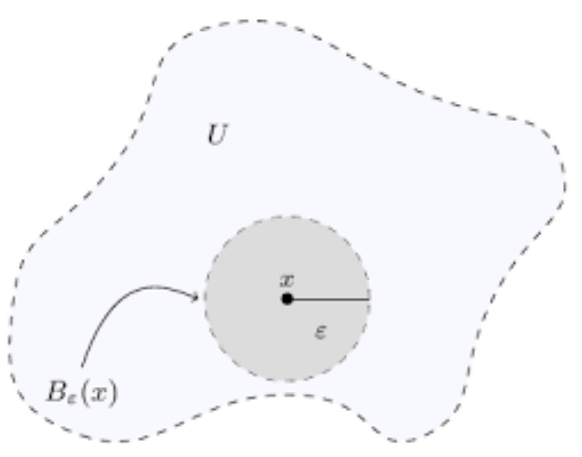
\includegraphics[width=8cm]{images/open_set.png}
    \caption{Open set}
\end{figure}

\section{Compactness}
\begin{defn}{Open cover}{}
By an \textbf{open cover} of a set $A$ in a metric space $X$ we mean a collection $\{G_\alpha\}$ of open subsets of $X$ such that $A \subset \bigcup_\alpha G_\alpha$.
\end{defn}

\begin{defn}{Compact set}{}
A subset $K$ of a topological (or metric) space is compact if every open cover of $K$ has a \emph{finite} subcover.
\end{defn}

An open cover of $A$ is a collection of open sets that collectively cover $A$.

A subcover is a subcollection of these open sets that still collectively cover $A$.

This means that any infinite collection of open sets that together cover a compact set always ``overcovers" it.

The simplest kind of compact set is just a finite set: a collection of finitely many points.

\pagebreak

\section{Some theorems}
\begin{thrm}{Cantor's Intersection Theorem}{}
Given a decreasing sequence of compact sets $A_1\supset A_2 \supset \cdots$, there exists a point $x\in\RR^n$ such that $x$ belongs to all $A_i$. In other words, $\bigcap_{i=1}^\infty A_i\neq\emptyset$. Moreover, if for all $i\in\NN$ we have $\diam A_{i+1}\le c\cdot\diam A_k$ for some constant $c<1$, then such a point must be unique, i.e. $\bigcap_{i=1}^\infty A_k=\{x\}$ for some $x\in\RR^n$.
\end{thrm}

\begin{thrm}{Heine-Borel Theorem}{}
A set $A\subset\RR^n$ is compact if and only if every open covering has a finite subcover, i.e. for any family of open sets $\mathscr{U}=\{U_i\}_{i\in I}$ satisfying $A\subset\bigcup_{i\in I}U_i$, there exists $\{U_1,\dots,U_n\}\subset\mathscr{U}$ such that $A\subset\bigcup_{i=1}^n U_i$.
\end{thrm}

\begin{thrm}{Bolzano-Weierstrass Theorem}{}
Infinite bounded sets in $\RR^n$ must contain limit points.
\end{thrm}

\begin{proof}
We will follow a very specific sequence of steps to prove them:
\begin{enumerate}
\item Cantor Intersection for $n=1$
\item Bolzano-Weierstrass for $n=1$
\item Bolzano-Weierstrass for general $n$
\item Cantor Intersection for general $n$
\item Heine-Borel for general $n$
\end{enumerate}

Proof:
\begin{enumerate}
\item Suppose that there is a decreasing sequence of compact sets $A_1, A_2, \dots$ in the real numbers

Since $A_k$ are bounded, we may let $a_k=\inf A_k$
Also since $A_k$ are closed, $a_k \in A_k$

Note that since $A_k$ is a decreasing sequence of sets we have $a_1\le a_2\le\dots$

Also, whenever we have $n>k$, we have $a_n \in A_n$, but $A_n \subset A_k$ and thus $a_n \in A_k$.

Let $b_1=\sup A_1$, then $a_k \in A_1$ and thus $a_k\le b_1$ for all $k$.

This tells us that the sequence $\{a_k\}$ is bounded above, and thus we may let $a=\sup a_k$.

Our goal is to show that the number $a$ appears in all $A_k$, thus showing that the entire intersection $\bigcap A_k$ contains $a$ and thus must be non-empty.

Now we split this in two cases, which asks whether a is simply made from isolated points, or if it is actually some nontrivial point obtained from the boundaries of $A_k$

\textbf{Case 1:} $a_k=a$ for some $k$
In this case we see that $a_k\le a_n\le a$ for all $n>k$ and thus $a_n=a$ in this case, therefore a is an element in $A_n$ for all $n$

In this case you can imagine that there is a possibility where a is an isolated minimum point of $A_n$ which stays there forever in the decreasing sequence of sets

\textbf{Case 2:} $a_k<a$ for all $k$; in this case we see that $a$ is the limit point of the increasing sequence $\{a_k\}$

Exercise 1: Show that $a$ is a limit point of each $A_k$.

Note that $a_n$ is in $A_k$ for each $n>k$, and since $a=\sup\{a_k\}$ where $a_k$ is increasing, we can actually show that a is a limit point of $\{a_n \mid n \le k\}$:
For every $\epsilon>0$, we pick $n_0$ such that $0 < a-a_{n_0} < \epsilon$
Pick $n\prime > \max\{k,n_0\}$, then $a_{n^\prime} \ge a_{n_0}$ and so
\[ 0<a-a_n\prime \le a_{n_0} < \epsilon \]
This shows that there exists $a_n^\prime$ in $B_0(a,\epsilon) \cap \{a_n \mid n>k\}$ for all $\epsilon$, and so $a$ is a limit point of $\{a_n \mid n>k\}$.

Now since $\{a_n|n \ge k\}$ is a subset of $A_k$ we also see that a is a limit point of $A_k$
Finally, since $A_k$ is closed, we conclude that $a$ is in $A_k$ for all $k$, and we are done

Wait hold on, I forgot about the second part

Now we consider a decreasing sequence of compact sets $A_1, A_2, \dots$ such that $\diam A_{k+1} \le c \diam A_k$ for $c<1$.

Suppose otherwise that there exists $x, y$ in $\bigcap A_k$

You can imagine that this will form a fixed distance between two points, and thus there is a constant positive lower bound for the diameters:
\[ \diam A_k \ge |x-y| > 0 \forall k \]

But this cannot be true because $\diam A_{k+1} \le c \diam A_k$ and so the diameter is controlled by a decreasing geometric sequence:
\[ \diam A_{k+1} \le c^k \diam A_1 \]

So we can simply pick a natural number $k$ such that
\[ k > \log_c \frac{|x-y|}{\diam A_1} \]

\item We consider an infinite bounded set $A$ in the real numbers. Since $A$ is bounded, we can pick a closed interval $[a_1,b_1]$ containing $A$.

We then perform a series of binary cuts: Consider the two halves of $[a_1,b_1]$. We know that at least one of these two must contain infinitely many elements in $A$, otherwise $A$ cannot be infinite. We pick this half of the interval and denote it by $[a_2,b_2]$. We continue this to pick a decreasing sequence of closed intervals $[a_n,b_n]$.

Now $\diam [a_{n+1},b_{n+1}] = \frac{1}{2} \diam [a_n,b_n]$, so by the Cantor Intersection Theorem, there exists a unique real number $c$ in the intersection $\bigcap[a_n,b_n]$.

We show that this $c$ is in fact a limit point of $A$.

For any $\epsilon>0$, we need to show that $B_0(c,\epsilon) \cap A \neq \emptyset$, i.e. we need to find an element $x \neq c$ in $A$ that is less than $\epsilon$ apart from $c$.

We then realize that we can simply exploit the decreasing sequence $[a_n,b_n]$
Since $\diam [a_n,b_n]$ is controlled by a decreasing sequence:
\[ \diam [a_{n+1},b_{n+1}] \le 1/2^n \diam [a_1,b_1] \]
We take a sufficiently large n so that $b_n-a_n<\epsilon$
Since $c$ is in $[a_n,b_n]$, for all $x$ in $[a_n,b_n]$ we have $|x-c|\le b_n-a_n<\epsilon$ and therefore $[a_n,b_n]$ is within $B(c,\epsilon)$.

Here's the funny part: $[a_n,b_n]$ contains infinitely many elements of $A$, so it must contain at least one element in A that is not $c$.

Therefore this element $x \neq c$ is in $B_0(c,\epsilon)$.

\item Now we have an infinte bounded set $A$ in $\RR^n$

The idea here is to consecutively come up with better and better sequences of points in $A$. We denote $x_i$ to be the $i$-th coordinate in $\RR^n$.

Our first wish is to pick some elements in $A$ so that they sort of converge at $x_1$.

Because such considerations of 'restricting to a single coordinate' is important here, we define the projection map to the $i$-th coordinate by
\[ f_i(x_1,\dots,x_n)=x_i \]

So, we look at $f_i(A)$ and try to apply BW for the case where $n=1$.

However, the problem is that $f_i(A)$ need not be infinite. For example, the set $\{(0,0),(0,1),(0,2),\dots\}$ projected onto the first coordinate is simply $\{0\}$.

This forces us to consider two cases

Exercise 2: Show that $f_i(A)$ is bounded
This is simple
1. $f_1(A)$ is infinite, then we can apply BW(n=1) to find a real number $c_1$ which is a limit point in $f_1(A)$

Here we can construct a sequence of points 
\[ \{x^{(1),1},x^{(1),2},...\} \]
so that their first coordinates satisfy
\[ |x^{(1),n}_1-c_1| < 1/n \]
for all natural number n
(I know this notation is cumbersome but the problem is that we need multiple sequences for this proof)

2. $f_1(A)$ is finite, then by the Pigeonhole Principle there exists a real number $c_1$ such that its preimage $f_1^{-1}(c_1)$ in $A$ is infinite

In this case we can randomly pick a sequence $\{x^{(1),1},x^{(1),2},\dots\}$ in $A$ so that their first coordinate is equal to $c_1$

I forgot to mention something that is implied, but we actually do have the need to emphasize that the sequence $\{x^{(1),1},x^{(1),2},\dots\}$ can be chosen to contain mutually distinct entries

Now that we have a sequence that behaves nice on the first coordinate, we may then move on to the second coordinate

Let $A_1=\{x^{(1),1},x^{(1),2},\dots\}$
We again consider $f_2(A_1)$ in two cases, infinite or finite

In any case, we are able to find a subsequence $\{x^{(2),1},x^{(2),2},\dots\}$, where
$x^{(2),k}=x^{(1),n_k}$ for some strictly increasing sequence of natural numbers $n_k$

So that, for the limit point/point with infinite preimage $c_2$, this sequence satisfies
\[ |f_2(x^{(2),n})-c_2| < \frac{1}{n} \]
Note that the property we have for the second case (we in fact have $f_2(x^{(2),n})=c_2$) is just a better version of this.

Now, take note that picking this subsequence does no harm whatsoever towards the first coordinate (if anything it would turn out to be better) since
\[ |f_1(x^{(2),k})-c_1| = |f_1(x^{(1),n_k}-c_1| < \frac{1}{n_k} \le \frac{1}{k} \]
($n_1<\dots<n_k$ is a strictly increasing sequence of natural numbers so $n_k \ge k$)

This continues on until we obtain a sequence of points $\{x^{(n),1},x^{(n),2},\dots\}$ in $A$ so that
\[ |f_i(x^{(n),k}-c_i|<\frac{1}{k} \quad \forall i,k \]

As we can see, the point $c=(c_1,\dots,c_n)$ is in fact a limit point of $A$ as we can always choose a big enough $k$ so that $x^{(n),k}$ is in $B(c,\epsilon) \cap A$.

Since $\{x^{(n),k}\}$ was always chosen to be a sequence of distinct entries, there is no danger for this sequence to always be c, and so c must be a limit point of $A$.

\item We may now return to the general case of Cantor.

Suppose that there is a sequence of decreasing compact sets $A_1,A_2,\dots$ in $\RR^n$. 
Note that every point is contained in $A_1$, so boundedness will never be an issue here.

Since $A_k$ are all nonempty, we can simply pick any element $a_k$ from $A_k$.

For the uncannily specific case that there are only finitely many $\{a_k\}$ chosen, we simply note that, again by Pigeonhole Principle, one of the $a_k$ appears infinitely often; thus for each $A_n$ we simply pick $n_k>n$ so that $A_{n_k}$ contains $a_k$, then $a_k$ is in $A_{n_k}$ which is a subset of $A_n$.

Otherwise, we can then note that $\{a_k\}$ is an infinite bounded set of points, so there must exist a limit point a of $\{a_k\}$.

We can now see that $a$ is always an element of $A_k$:
Using the same technique as Exercise 1, we see that a is a limit point of $\{a_n \mid n>k\}$ and so is a limit point of $A_k$, therefore a is in $A_k$ as $A_k$ is closed.

This proves the first part of the statement
The second part is completely identical to the second part of the $n=1$ case so we don't need to waste our time there either

\item We now consider a compact set A with some open covering $\mathscr{U}$.

This theorem is proved by contradiction: 
Suppose otherwise that set $A$ cannot be covered by any finite collection of open sets in $\mathscr{U}$

Since $A$ is compact, we may enclose it in a closed cube $Q_1$ (whose edges are parallel to the axes)

Now, for each step, we partition $Q$ into $2^n$ cubes by cutting it in half from each direction.

Then, starting from $Q_1$, there must exist one of these smaller cubes, denoted by $Q_2$, such that $A \cap Q_2$ cannot be covered by a finite collection of open sets in $\mathscr{U}$. 
Otherwise, if each $A \cap Q$ has a finite cover, then we simply collect all of these open sets together to form a finite cover of $A$, which violates our assumption.

We continue on to partition $Q_n$ and pick $Q_{n+1}$ so that $A_{n+1}$ has no finite cover (denote $A_n = A \cap Q_n$).

Note that $A$ and $Q_n$ are both compact, so $A_n$ is compact
Also we see that there is a decreasing sequence $A_1,A_2,\dots$
(we can't exactly obtain a relation between $\diam A_n$ and $\diam A_{n+1}$ here)

By Cantor Intersection Theorem we can always find a point $x$ in $A$ located in the intersection $\bigcap A_k$.

Now, since $\mathscr{U}$ is an open covering of $A$, there exists an open set $U$ in $\mathscr{U}$ such that $x\in U$.

The final key step is to exploit the sequence of decreasing cubes $Q_n$. So even though there isn't a clear cut way to control the sizes of $\diam A_n$, we do in fact have the property that $\diam Q_{n+1} = \frac{1}{2^n} \diam Q_1$.

Therefore, by picking a sufficiently large $n$, we can obtain $Q_n$ that is contained in $U$.

But this is a contradiction. 
This is because we've specifically chosen the sequence $A_n$ to be sets that do not possess any finite cover $\{U_1,...,U_n\}$ in $\mathscr{U}$. But here $A_n$ simply would have a one-element cover $\{U\}$.

This completes our proof.
\end{enumerate}
\end{proof}

\chapter{Metric Spaces (to remove)}

\section{Structures on Euclidean Space}
\begin{defn}{Limit and isolated point}{}
A point $p$ is a limit point of $E$ if every neighborhood of $p$ contains a point $q \neq p in E$. 

If $p$ is not a limit point but is in $E$, then $p$ is an isolated point.
\end{defn}

\begin{defn}{Closed set}{}
$E$ is closed if every limit point of $E$ is in $E$. Intuitively, this means $E$ ``contains all its edges".

The closure $\bar{E}$ of $E$ is the union of E and the set of its limit points.
\end{defn}

\begin{defn}{Interior point}{}
A point $p$ is an interior point of $E$ if there is a neighborhood $N$ of $p$ such that $N \subset E$. Note that interior points must be in $E$ itself, while limit points need not be.
\end{defn}

\begin{defn}{Open set}{}
E is open if every point of E is an interior point of E. Intuitively, E “doesn’t have edges”.
\end{defn}

\begin{defn}{Dense set}{}
E is dense in X if every point of X is a limit point of E or a point of E, or both.
\end{defn}

\begin{defn}{Interior}{}
The interior $E^0$ of $E$ is the set of all interior points of $E$, or equivalently the union of all open sets contained in $E$.
\end{defn}

\subsection{Some Concepts in Euclidean Space}
\begin{defn}{Bounded set}{}
A set $E$ in $\RR^n$ is a \vocab{bounded set} if there exists $M>0$ such that $\forall x \in E,\:\norm{x} \le M$.
\end{defn}

\begin{prbm}
$E,F$ in $\RR^n$ and real $k$, define
\[ kE = \{kx \mid x \in E\} \]
\[ E+F = \{x+y \mid x \in E,y \in F\} \]
\begin{enumerate}[label=(\alph*)]
\item Show that if $E$ is bounded, then $kE$ is bounded;
\item Show that if $E$ and $F$ are bounded, then $E+F$ is bounded
\end{enumerate}
\end{prbm}

\begin{defn}{Diameter of set}
Given a set $E \subset \RR^n$, the \vocab{diameter} of $E$ is defined as 
\[ \diam E = \sup_{x,y\in E} d(x,y). \]
\end{defn}

\begin{prbm}
Find the diameter of the open unit ball in $\RR^n$ given by
\[ B = \{x \in \RR^n \mid \norm{x}<1\} \]
\end{prbm}

\begin{proof}[Solution]
First note that
\[ d(x,y) = \norm{x-y} \le \norm{x}+\norm{-y} = \norm{x}+\norm{y} <1+1=2 \]

On the other hand, for any $\epsilon>0$, we pick
\[ x=(1-\frac{\epsilon}{4},0,\dots,0), y=(-\brac{1-\frac{\epsilon}{4}},0,\dots,0) \]
Then
\[ d(x,y) = 2-\frac{\epsilon}{2} > 2-\epsilon \]

Therefore $\diam B = 2$.
\end{proof}

\begin{prbm}
Given a set $E$ in $\RR^n$, show that $E$ is bounded if and only if $\diam E < +\infty$.
\end{prbm}

\begin{proof}[Solution] \ {\\}
\textbf{Forward direction}:

If $E$ is bounded, then there exists $M>0$ such that $\forall x \in E$, $\norm{x} \le M$.

Thus $\forall x,y \in E$,
\[ d(x,y) = \norm{x-y} \le \norm{x} + \norm{y} \le 2M. \]
Thus $\diam E = \sup d(x,y) \le 2M < +\infty$

\textbf{Backward direction}:

Suppose that $\diam E = r$.

Pick a random point $x \in E$, suppose that $||x||=R$

Then for any other $y \in E$,
\[ \norm{y} = \norm{x+(y-x)} \le \norm{x} + \norm{y-x} \le R+r \]

Thus, by picking $M=R+r$, we obtain $\norm{y} \le M \forall y \in E$, and we're done.

Basically you use $x$ to confine $E$ within a ball, which is then confined within an even bigger ball centered at the origin.
\end{proof}

\begin{defn}{Distance between sets}{}
Given two sets $E,F \subset \RR^n$, the \vocab{distance between sets} $E$ and $F$ is defined as 
\[ d(E,F) = \inf_{x\in E, y\in F}\norm{x-y}. \]
\end{defn}

Obviously $d(E,F)>0$ implies that $E$ and $F$ are disjoint, but $E$ and $F$ may still be disjoint even if $d(E,F)=0$, e.g. the closed intervals $E=(-1,0), F=(0,1)$.

\begin{prbm}
Suppose that $E$ and $F$ are sets in $\RR^n$ where $F$ is finite, then $E$ and $F$ are disjoint if and only if $d(E,F)>0$.
\end{prbm}

Topology in Euclidean Space

Before we move on, we need to talk about how we think about topology. The concept first begins with an attempt to say that two points are close to one another. 

Of course, we did define the metric earlier
But as it turns out, this particular notion can be made extremely abstract

Specifically speaking, we could theoretically define closeness simply with set theory

Imagine that in some random set X, there is a predetermined family of subsets scrA in P(X)
(scr: script; cursive)

Now for some element x in X, suppose that we can pick a set in $\mathscr{A}$ containing $x$. 

We may denote this set as U(x)
Then, from the perspective of U(x), a point y in X would seem to be close to x if y also lies in U(x)

Ah actually the family of subsets is usually denoted as $\mathscr{N}$

The family $\mathscr{N}$ is called the neighbourhood system

There is also the notion of the neighbourhood system of a particular point,
\[ \mathscr N(x) = \{U \in \mathscr{N} \mid x \in U\} \]

Now, here's the easiest part to confuse
:
The word 'system' in the above terminology is actually quite crucial
It is not named 'neighbourhood set' or 'neighbourhood family' for a reason
:
That's because the terminology of 'neighbourhood' is used as follows:
We say that a subset of X, let's say N, is a neighbourhood of x, if there is some neighbourhood $U \in \mathscr{N}$ such that $x \in U$ and $U \subset N$.
:
Ah I'm very sorry but I messed up the terminology

According to wikipedia, the neighbourhood system actually refers to all neighbourhoods
What I was talking about earlier should've been called a neighbourhood basis

:
The neighbourhood basis is denoted by scrB



Okay let's redo the entire thing

1. Neighbourhood Basis
Given a set $X$, we define a family of subsets in $X$, denoted by $scrB$, to describe points close to each other; points that belong to the same set $U$ in $scrB$ are considered to be close to each other with respect to $U$.

2. Neighbourhood
Given a point $x$ in $X$, we use the term \vocab{neighbourhood} to describe a particular construction for $x$; $N$ is said to be a neighbourhood of $x$, if there exists $U$ in $\mathscr{B}$ containing $x$ such that $U \subset N$.

2'. Neighbourhood System
Given a point $x$ in $X$, the \vocab{neighbourhood system} of $x$, denoted $\mathscr{N}(x)$, is the set of all neighbourhoods of $x$.

These are the axioms for the neighbourhood systems
\begin{enumerate}
\item $\mathscr{N}(x)$ is nonempty, and $\forall U \in \mathscr{N}(x), x \in U$
\item If $U,V \in \mathscr{N}(x)$, then $\exists W \in \mathscr{N}(x) \suchthat W \subset U \cap V$
\item If $U \in \mathscr{N}(x)$ and $y \in U$, then $\exists V \in \mathscr{N}(y) \suchthat V \subset U$
\end{enumerate}

As for the Euclidean plane, we have a natural way of defining the neighbourhood systems
First we pick the neighbourhood basis to be
\[ \mathscr{B} = \{B(x,\epsilon) \mid x \in \RR^n,\epsilon>0\} \]

Then we say that N is a neighbourhood of x if there exists $\epsilon>0$ such that $B(x,\epsilon) \subset N$. 
$B(x,\epsilon)$ represents the points close to x, whereas a neighbourhood N of x should contain all the points close to x, at least from the perspective of $B(x,\epsilon)$

Once we have neighbourhood systems, we can then define the two most important kinds of sets in topology, open and closed sets.


\chapter{Knot Theory}
\textbf{Readings:}
\begin{itemize}
\item \href{https://stanford.edu/~sfh/knot.pdf}{Knot Theory by Stanford University}
\item \href{https://www.math.cuhk.edu.hk/course_builder/1920/math4900e/Adams--The%20Knot%20Book.pdf}{The Knot Book by Colin C. Adams}
\end{itemize}

\section{Knot and Knot Types}

\part{Complex Analysis}
\chapter{Functions}
\textbf{Readings:} Visual Complex Analysis by Needman

\section{Complex Functions}
\subsection{Exponential function}
We have Euler's formula: $e^{i\theta} = \cos\theta + i\sin\theta$. We can extend this to the complex exponential function $e^z$.

\begin{defn}{Complex exponential function}{}
For $z=x+iy$ the \vocab{complex exponential function} is defined as
\[ e^z = e^{x+iy} = e^xe^{iy} = e^x(\cos y + i\sin y). \]
\end{defn}

In this definition $e^x$ is the usual exponential function for a real variable $x$. It is easy to see that all the usual rules of exponents hold:
\begin{itemize}
\item $e^0 = 1$

\item $e^{z_1+z_2} = e^{z_1} e^{z_2}$

\item $(e^z)^n = e^{nz}$ for positive integers $n$.

\item $(e^z)^{-1} = e^{-z}$

\item $e^z \neq 0$

It will turn out that the property $\dv{e^z}{z}=e^z$ also holds, but we can't prove this yet because we haven't defined what we mean by the complex derivative d/dz. 

\item $|e^{i\theta}| = 1$
\begin{proof}
\[ |e^{i\theta}| = |\cos\theta+i\sin\theta| = \sqrt{\cos^2\theta+\sin^2\theta} = 1 \]
\end{proof}

\item $|e^{x+iy}| = e^x$
(as usual z = x + iy and x, y are real).

\item The path $e^{it}$ for $0<t<\infty$ wraps counterclockwise around the unit circle. It does so infinitely many times.
\end{itemize}

\subsection{Complex functions as mappings}
\subsection{Function $\arg z$}
3.3.1 Many-to-one functions . . . . . . . . . . . . . . . . . . . . . . . . . . 25
3.3.2 Branches of arg(z) . . . . . . . . . . . . . . . . . . . . . . . . . . . . 26
3.3.3 The principal branch of arg(z) . . . . . . . . . . . . . . . . . . . . . 28
\subsection{Branches and branch cuts}
\subsection{Function $\log z$}
3.5.1 Figures showing w = log(z) as a mapping . . . . . . . . . . . . . . . 30
3.5.2 Complex powers . . . . . . . . . . . . . . . . . . . . . . . . . . . . . 32

\section{Analytic Functions}
\subsection{The derivative: preliminaries}
\subsection{Open disks, open deleted disks, open regions}
\subsection{Limits and continuous functions}
4.3.1 Properties of limits . . . . . . . . . . . . . . . . . . . . . . . . . . . . 36
4.3.2 Continuous functions . . . . . . . . . . . . . . . . . . . . . . . . . . . 36
4.3.3 Properties of continuous functions . . . . . . . . . . . . . . . . . . . 37
\subsection{The point at infinity}
4.4.1 Limits involving infinity . . . . . . . . . . . . . . . . . . . . . . . . . 38
4.4.2 Stereographic projection from the Riemann sphere . . . . . . . . . . 39
\subsection{Derivatives}
4.5.1 Derivative rules . . . . . . . . . . . . . . . . . . . . . . . . . . . . . . 40
\subsection{Cauchy-Riemann equations}
4.6.1 Partial derivatives as limits . . . . . . . . . . . . . . . . . . . . . . . 41
4.6.2 The Cauchy-Riemann equations . . . . . . . . . . . . . . . . . . . . 42
4.6.3 Using the Cauchy-Riemann equations . . . . . . . . . . . . . . . . . 43
4.6.4 f0(z) as a 2 × 2 matrix . . . . . . . . . . . . . . . . . . . . . . . . . . 44
4.7 Geometric interpretation \& linear elasticity theory . . . . . . . . . . . . . . 45
4.8 Cauchy-Riemann all the way down . . . . . . . . . . . . . . . . . . . . . . . 46
4.9 Gallery of functions . . . . . . . . . . . . . . . . . . . . . . . . . . . . . . . 47
4.9.1 Gallery of functions, derivatives and properties . . . . . . . . . . . . 47
4.9.2 A few proofs . . . . . . . . . . . . . . . . . . . . . . . . . . . . . . . 51
4.10 Branch cuts and function composition . . . . . . . . . . . . . . . . . . . . . 52
4.11 Appendix: Limits . . . . . . . . . . . . . . . . . . . . . . . . . . . . . . . . . 54
4.11.1 Limits of sequences . . . . . . . . . . . . . . . . . . . . . . . . . . . . 54
4.11.2 limz→z0
f(z) . . . . . . . . . . . . . . . . . . . . . . . . . . . . . . . . . 56
4.11.3 Connection between limits of sequences and limits of functions . . . 56

\part{Discrete Mathematics}
\chapter{Graph Theory}
% Clear this first: https://web.evanchen.cc/notes/SJSU179.pdf
% http://web.mit.edu/yufeiz/www/imo2008/tang-graph.pdf
% https://yufeizhao.com/211/graph_theory_notes.pdf
% https://courses.maths.ox.ac.uk/pluginfile.php/78926/mod_resource/content/0/Lecture%20notes.pdf
% https://books.google.com.cu/books?id=7_bQa4SJTQQC&printsec=frontcover#v=onepage&q&f=false

\section{Definitions}
\subsection{Preliminary Definitions}
\begin{defn}{Graph}{}
A \vocab{graph} $G = (V(G),E(G))$ consists of two sets $V(G)$ (the \textbf{vertex} set) and $E(G)$ (the \textbf{edge} set), where each element of $E(G)$ consists of a pair of elements of $V(G)$. 
\end{defn}

\begin{notation}
$|G|=|V(G)|$ denotes the number of vertices and $e(G) =|E(G)|$ denotes the number of edges.
\end{notation}

The \textbf{order} of a graph $G$ is $|V(G)|$. The \textbf{size} of $G$ is $|E(G)|$.

We represent $G$ visually by drawing a point for each vertex and a line between any pair of points that form an edge.

The \vocab{complement} of $G$, denoted by $\overline{G}$, is a graph with the same vertex set as $G$ and $E(\overline{G}) = \{e \notin E(G)\}$, i.e. $\overline{G}$ has edges exactly where there are no edges in $G$.

\begin{defn}{Simple graph}{}
A loop is an edge $(v,v)$ for some $v \in V$. An edge $e = (u,v)$ is a multiple edge if it appears multiple times in $E$. 

A graph is \vocab{simple} if it has no loops or multiple edges.
\end{defn}

\begin{remark}
Unless explicitly stated otherwise, we will only consider simple graphs. General (potentially non-simple) graphs are also called multigraphs.
\end{remark}

Vertices $u$ and $v$ are \textbf{neighbours} if $(u,v) \in E(G)$; we also say that $u$ and $v$ are \textbf{adjacent}. An edge $e \in E(G)$ is \textbf{incident} to a vertex $v \in V(G)$ if $v \in e$. Edges $e, e^\prime$ are \textbf{incident} if $e \cap e^\prime = \emptyset$.

Given a vertex $v$, the \textbf{degree} of $v$, denoted by $d(v)$, is the number of neighbours of $v$ in $G$. If the degree of each vertex is the same, we can call that the degree of the graph. A \textbf{leaf} is a vertex of degree one, i.e. with a unique neighbour.

\begin{remark}
A trivial graph is a graph with order 1. An empty graph is a graph of size 0. 
Note that a graph must have at least one vertex by definition. But a graph can certainly have no edges!
\end{remark}

\subsection{Subgraph}
\begin{defn}{Subgraph}{}
$H$ is a \vocab{subgraph} of $G$ if $V(H) \subseteq V(G)$ and $E(H) \subseteq E(G)$.
\end{defn}

$H$ is a \vocab{spanning subgraph} if $V(H)=V(G)$.

$H$ is an \vocab{induced subgraph} if $(u,v) \in E(H) \iff (u,v) \in E(G) \forall u, v \in V(H)$.

\subsection{Walks}
\begin{defn}{Walk}{}
A \vocab{$u-v$ walk} in $G$, denoted by $W$, is a finite sequence of vertices $u=v_0,v_1,\dots,v_k=v$ such that $v_i v_{i+1} \in E(G)$ for all $0 \le i < k-1$.
\end{defn}

A walk is \textbf{closed} if and only if $u=v$. Otherwise, it is \textbf{open}.

A \vocab{trail} is an open walk without repeating vertices.

A \vocab{path} is an open walk without repeating edges.
Note that paths are trails, but not vice-versa.

A \vocab{circuit} is a closed walk without repeating edges, i.e. $u=v$, it begins and ends with the same vertex.

A \vocab{cycle} is a closed walk without repeating vertices, other than the initial and terminal vertices, i.e. $u=v$ but the vertices are otherwise distinct and $W$ has at least 3 vertices. If a graph $G$ has no cycle we call it \textbf{acyclic}.

A \vocab{trail} is a walk in which no two vertices appear consecutively (in either order) more than once; that is, no edge is used more than once. A \vocab{tour} is a closed trail.

\subsection{Connectedness}
\begin{defn}{Connected}{}
A graph $G$ is \vocab{connected} if $\forall u,v \in V(G)$ there exists a $u-v$ path.
\end{defn}

Let $G$ be a connected graph. Then $d(u,v)$ is the \textbf{smallest length} of any $u-v$ path if $u \neq v$, or 0 if $u=v$.

The \textbf{diameter} of a connected graph $G$, denoted by $\diam G$, is defined as
\[ \diam G = \max_{u\neq v} d(u,v). \]
By construction, $d(u,v) \le \diam G \forall u,v \in V(G)$.

We say that two vertices $u$ and $v$ of a graph $G$ lie in the same \textbf{component} if they are joined by an $u-v$ walk. Clearly this forms an equivalence relation and the partition of $V(G)$ into equivalence classes expresses $G$ as a union of disjoint connected graphs called its components.

$G$ is \vocab{complete} if every pair of vertices in $G$ is joined by an edge. A complete graph on $n$ vertices is denoted by $K_n$.

\subsection{Classes of graphs}
\vocab{Empty graph}: We let $E_n$ denote the empty graph with order $n$ and size 0. This graph is disconnected if and only if $n \ge 2$.

\vocab{Path graph}: We let $P_n$ be the graph of order $n$ and size $n-1$. You can guess what this is: It is connected with diameter $n-1$.

\vocab{Cycle graph}: We let $C_n$ denote the graph of order $n$ and size $n$ which consists of a single
cycle. Note that $n \ge 3$. It is connected with diameter $\floor{\frac{1}{2}n}$.

\vocab{Complete graph}: We let $K_n$ denote the complete graph, with order $r$ and size $\binom{n}{2}$. It is extremely connected with diameter 1 (for $n \ge 2$). Note that this is the only class of connected graphs with diameter 1.

Note that $E_1 = K_1 = P_1$, $K_2 = P_2$ and $K_3 = C_3$.

\subsection{Bipartite Graphs}
$G$ is \vocab{bipartite} if $V(G)$ can be partitioned into two non-empty disjoint sets $A$ and $B$ such that no edge has both endpoints in the same set. A graph is said to be \textbf{complete bipartite} if $G$ is bipartite and all possible edges between the two sets $A$ and $B$ are drawn. In the case where $|A|=m, |B|=n$, such a graph is denoted by $K_{m,n}$.

Let $k \ge 2$. A graph $G$ is said to be \textbf{$k$-partite} if $V(G)$ can be partitioned into $k$ pairwise disjoint sets $A_1, \dots, A_k$ such that no edge has both endpoints in the same set. A \textbf{complete $k$-partite} graph is defined similarly as a complete bipartite. In the case where $|A_i| = n_i$, such a graph is denoted by $K_{n_1,n_2,\dots,n_k}$.

A graph is \vocab{planar} if it can be drawn such that a pair of edges can only cross at a vertex.

\begin{thrm}{Euler's Characteristic Formula}{}
For any connected planar graph, the number of vertices $V$ minus the number of edges $E$ plus the number of regions $R$ equals 2. 
\begin{equation} V-E+R = 2 \end{equation}
\end{thrm}

(or V-E+F=2 for 3 dimensional polyhedra)
To prove this, 
for trivial graph, V=1, F=1, E=0
Adding one edge, we either introduce a new vertex or face (if edge is connected to preexisting vertex)



\subsection{Isomorphism}
\begin{defn}{Isomorphism}{}
Let $G_1 = (V_1, E_1)$ and $G_2 = (V_2, E_2)$ be graphs. An isomorphism $\phi : G_1 \to G_2$ is a bijection (a one-to-one correspondence) from $V_1$ to $V_2$ such that $(u,v) \in E_1$ if and only if $(\phi(u),\phi(v)) \in E_2$. We say $G_1$ is isomorphic to $G_2$ if there is an isomorphism between them.
\end{defn}



\section{Trees and Balancing}
A \vocab{tree} is defined to be a connected graph that does not contain any cycles; to put it simply, it is a minimally connected graph.

A \vocab{cycle} in a graph means there is a path from an object back to itself.

Characterisation of trees: Let $G$ be a connected graph with $n$ vertices. The following statements are equivalent.
\begin{enumerate}
\item $G$ does not contain any cycles
\item $G$ contains exactly $n-1$ edges
\item For any two vertices, there exists exactly one path joining the two vertices
\item The removal of any edge disconnects the graph
\end{enumerate}

\begin{lemma}\label{acyclic}
Any tree is acyclic.
\end{lemma}
\begin{proof}
Let $G$ be a tree, i.e. $G$ is minimally connected. Suppose for a contradiction that $G$ contains a cycle $C$. Let $e \in E(C)$. We will obtain our contradiction by showing that $G-e \coloneqq (V(G),E(G)\setminus\{e\})$ is connected. 

Let $P$ be the path obtained by deleting $e$ from $C$. Consider any $u,v$ in $V(G)$. As $G$ is connected, there is an $u-v$ walk $W$ in $G$. Replacing any use of $e$ in $W$ by $P$ gives an $u-v$ walk in $G-e$. Thus $G-e$ is connected, a contradiction.
\end{proof}

There are many equivalent characterisations of trees, any of which could be taken as the definition. Here is one:

\begin{lemma}\label{tree_iff}
$G$ is a tree if and only if $G$ is connected and acyclic.
\end{lemma}
\begin{proof}
If $G$ is a tree then $G$ is connected by definition and acyclic by \cref{acyclic}. Conversely, let $G$ be connected and acyclic. Suppose for a contradiction that $G-e$ is connected for some $e = (u,v) \in E(G)$.

Let $W$ be a shortest $u-v$ walk in $G-e$. Then $W$ must be a path, i.e. have no repeated vertices, otherwise we would find a shorter walk by deleting a segment of $W$ between two visits to the same vertex. Combining $W$ with $(u,v)$ gives a cycle, which is a contradiction.
\end{proof}

\begin{remark}
The fact that a shortest walk between two points is a path is often useful. More generally, considering an extremal (shortest, longest, minimal, maximal, \dots) object is often a useful proof technique.
\end{remark}

\begin{lemma}
Any two vertices in a tree are joined by a unique path.
\end{lemma}
\begin{proof}
Suppose for a contradiction that this fails for some tree $G$. 

Choose $u,v$ in $V(G)$ so that there are distinct $u-v$ paths P1, P2, and P1 is as short as possible over all such choices of $u$ and $v$.

Then P1 and P2 only intersect in $u$ and $v$, so their union is a cycle, contradicting \cref{acyclic}.
\end{proof}

\begin{lemma}\label{tree_leaves}
Any tree with at least two vertices has at least two leaves.
\end{lemma}
\begin{proof}
Consider any tree $G$. Let $P$ be a longest path in $G$. The two ends of $P$ must be leaves. Indeed, an end cannot have a neighbour in $V(G) \setminus V(P)$, or we could make $P$ longer, and cannot have any neighbour in $V(P)$ other than the next in the sequence of $P$, or we would have a cycle.

The existence of leaves in trees is useful for inductive arguments, via the following lemma. Given $v \in V(G)$, let $G-v$ be the graph with $V(G-v) = V(G)\setminus\{v\}$ and $E(G-v) = \{(u,v) \in E(G) \mid v \notin \{u,v\}\}$.
\end{proof}

\begin{lemma}\label{tree_leaf}
If $G$ is a tree and $v$ is a leaf of $G$ then $G-v$ is a tree.
\end{lemma}
\begin{proof}
By \cref{tree_iff} it suffices to show that $G-v$ is connected and acyclic. Acyclicity is immediate from \cref{acyclic}. Connectedness follows by noting for any $u,v \in V(G)\setminus\{v\}$ that the unique $u-v$ path in $G$ is contained in $G-v$.
\end{proof}

\begin{lemma}\label{tree_edges}
Any tree on $n$ vertices has $n-1$ edges.
\end{lemma}
\begin{proof}
By induction. A tree with 1 vertex has 0 edges. Let $G$ be a tree on $n>1$ vertices. By \cref{tree_leaves}, $G$ has a leaf $v$. By \cref{tree_leaf}, $G-v$ is a tree. By induction hypothesis, $G-v$ has $n-2$ edges. Replacing $v$ gives $n-1$ edges in $G$.
\end{proof}

We conclude this section with another characterisation of trees. First we note that any connected graph $G$ contains a minimally connected subgraph (i.e. a tree) with the same vertex set, which we call a \vocab{spanning tree} of $G$.

\begin{lemma}
A graph $G$ is a tree on $n$ vertices if and only if $G$ is connected and has $n-1$ edges.
\end{lemma}
\begin{proof}
If $G$ is a tree then $G$ is connected by definition and has $n-1$ edges by \cref{tree_edges}. 

Conversely, suppose that $G$ is connected and has $n-1$ edges. Let $H$ be a spanning tree of $G$. Then $H$ has $n-1$ edges by \cref{tree_edges}, so $H = G$, so $G$ is a tree.
\end{proof}

\section{Euler Tours and Trails}
An \vocab{Euler trail} is a trail in which every pair of adjacent vertices appear consecutively. (That is, every edge is used exactly once.)

An \vocab{Euler tour} is a closed Euler trail.


vertex/edge colouring and Ramsey Theory

Regular graph
Directed graph

graph concepts such as Shortest-, Euler-, Hamilton-Paths and Cycles, coloring, planarity, weighted graphs, and directed graphs.

Topics in graph theory, including: connectivity and matchings, Hall's theorem, Menger's theorem, network flows; paths and cycles, complete subgraphs and Turán's theorem, and the Erdös-Stone theorem; graph colouring and the four-colour theorem; Ramsey theory; probabilistic methods in graph theory; and the use of software to solve graph-theoretic problems.
\pagebreak

\section*{Problems}
\begin{prbm}[K\"{o}nigsberg Bridge Problem]
K\"{o}nigsberg was a small town in Prussia. There is a river running through the town and there were seven bridges across the river. The inhabitants of K\"{o}nigsberg liked to walk around the town and cross all of the bridges:

Is it possible to walk around the town and cross every bridge, once and once only?
\end{prbm}

\begin{solution}
We replace every landmass by a vertex and every bridge by an edge to give the following graph.


\end{solution}
\pagebreak

Problems can include tournament, matching, and scheduling problems.
\begin{prbm}(Moser's circle problem) 
Determine the number of regions into which a circle is divided if $n$ points on its circumference are joined by chords with no three internally concurrent.
\end{prbm}

\begin{proof}[Solution]
Consider the graph which has points on the circumference and intersection points between chords as its vertices.

Let $V, E, F$ denote the number of vertices, edges, regions respectively.

To count the number of intersection points, note that $4$ points on the circumference give one unique intersection point between the two non-parallel chords formed by connecting two pairs of points which intersect inside the circle. Hence, number of intersection points is $\dbinom{n}{4}$. 
\[ V = n + \binom{n}{4} \]
Total number of edges includes $n$ circular arcs, number of original chords formed from connecting pairs of points on the circumference
E = no. of original lines + 2 x no. of intersection points
E = n choose 2 + 2 x n choose 4 + n
since there are n circular arcs

Using Euler's Characteristic Formula, we have 
\begin{align*}
F &= E - V - 1 \\
\Aboxed{F &= 1 + \binom{n}{2} + \binom{n}{4}}
\end{align*}
\end{proof}

\chapter{Game Theory}
\textbf{Recommended readings:} \href{https://mathematicalolympiads.files.wordpress.com/2012/08/martin_j-_osborne-an_introduction_to_game_theory-oxford_university_press_usa2003.pdf}{``An Introduction to Game Theory" by Osborne}

% games of normal form and extensive form, and their applications in economics, relations between game theory and decision making; games of complete information: static games with finite or infinite strategy spaces, Nash equilibrium of pure and mixed strategy, dynamic games, backward induction solutions, information sets, subgame-perfect equilibrium, finitely and infinitely-repeated games; games of incomplete information: Bayesian equilibrium, first price sealed auction, second price sealed auction, and other auctions, dynamic Bayesian games, perfect Bayesian equilibrium, signaling games; cooperative games: bargaining theory, cores of n-person cooperative games, the Shapley value and its applications in voting, cost sharing, etc.

Game Theory is the study of strategically interdependent behaviour.
\section{Strict Dominance}
\subsection{Prisoner's Dilemma}
To start off, we will take a look at the \vocab{Prisoner's Dilemma}, which goes as follows:

\begin{ebox}
Two thieves plan to rob a store, but the police arrest them for trespassing. The police suspect that they planned to break in but lack the evidence to support such an accusation. They require a confession to charge the suspects. The police offer them the following deal:
\begin{itemize}
\item If no one confesses, both are charged a \emph{one month} jail sentence each for trespassing.
\item If a rat confesses and the other does not, the rat is not charged but the other is charged a \emph{twelve month} jail sentence for robbery.
\item If both confess, both are charged an \emph{eight month} jail sentence each.
\end{itemize}
If both criminals are self-interested and only care about minimising their jail time, should they take the interrogator's deal?
\end{ebox}

We condense the above information into a \vocab{payoff matrix} as shown below, where we have two players, A and B. The horizontal rows represent A's choices, while the vertical columns represent B's choices, and each cell contains a combination of their payoffs.

\begin{table}[H]
\centering
\begin{tabular}{rcc}
\multicolumn{1}{l}{}         & quiet                       & confess                     \\ \cline{2-3} 
\multicolumn{1}{r|}{quiet}   & \multicolumn{1}{c|}{$-1$, $-1$} & \multicolumn{1}{c|}{$-12$, $0$} \\ \cline{2-3} 
\multicolumn{1}{r|}{confess} & \multicolumn{1}{c|}{$0$, $-12$} & \multicolumn{1}{c|}{$-8$, $-8$} \\ \cline{2-3} 
\end{tabular}
\end{table}

\subsection{Split or Steal}
The game goes as follows:
\begin{ebox}
Each of two players, Sarah and Steve, has to pick one of two balls: inside one ball appears the word ‘\textbf{split}’ and inside the other the word ‘\textbf{steal}’ (each player is first asked to secretly check which of the two balls in front of him/her is the split ball and which is the steal ball). They make their decisions simultaneously. 
\end{ebox}

The possible outcomes are shown in the figure below, where each row is labelled with a possible choice for Sarah and each column with a possible choice for Steven. Each cell in the table thus corresponds to a possible pair of choices and the resulting outcome is written inside the cell.

\begin{figure}[H]
    \centering
    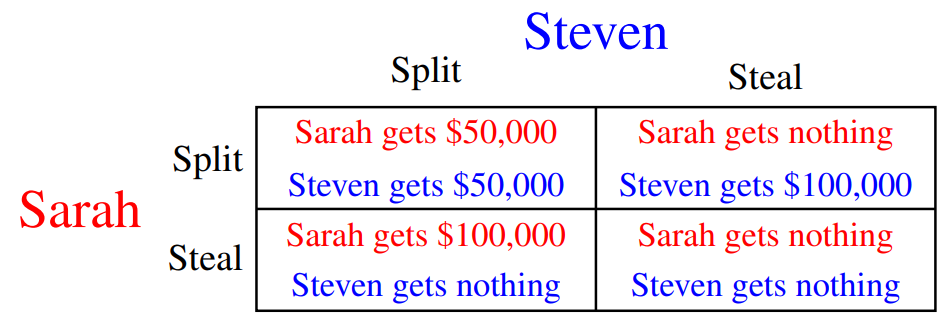
\includegraphics[width=12cm]{images/Split_or_steal.png}
\end{figure}

\section{Nash Equilibrium}
\textbf{Nash Equilibrium} is a set of optimal strategies that work against \textit{all} counter-steategies. This means that if any given player were told the strategies of all their opponents, they still would choose to retain their original strategy. 

\subsection{Matrix games}

\section{Fair Division}
\subsection{Rental harmony problem}
Sperner's lemma

https://www.cs.cmu.edu/~arielpro/15896/docs/paper19b.pdf

\end{document}